\documentclass[11pt,oneside]{book}



%%%%%%%%%%%%%%Include Packages%%%%%%%%%%%%%%%%%%%%%%%%%%
\usepackage{xcolor}
\usepackage{mathtools}
\usepackage[legalpaper, margin=1in]{geometry}
\usepackage{amsmath}
\usepackage{amssymb}
\usepackage{paralist}
\usepackage{rsfso}
\usepackage{amsthm}
\usepackage{wasysym}
\usepackage[inline]{enumitem}   
\usepackage{hyperref}
\usepackage{tocloft}
\usepackage{wrapfig}
\usepackage{titlesec}
%%%%%%%%%%%%%%%%%%%%%%%%%%%%%%%%%%%%%%%%%%%%%%%%%%%%%%%%


%%%%%%%%%%%%%%%Chapter Setting%%%%%%%%%%%%%%%%%%%%%%%%%%
\definecolor{gray75}{gray}{0.75}
\newcommand{\hsp}{\hspace{20pt}}
\titleformat{\chapter}[hang]{\Huge\bfseries}{\thechapter\hsp\textcolor{gray75}{$\mid$}\hsp}{0pt}{\Huge\bfseries}
%%%%%%%%%%%%%%%%%%%%%%%%%%%%%%%%%%%%%%%%%%%%%%%%%%%%%%%%

%%%%%%%%%%%%%%%%%Theorem environments%%%%%%%%%%%%%%%%%%%
\newtheoremstyle{break}
  {\topsep}{\topsep}%
  {\itshape}{}%
  {\bfseries}{}%
  {\newline}{}%
\theoremstyle{break}
\theoremstyle{break}
\newtheorem{axiom}{Axiom}
\newtheorem{thm}{Theorem}[section]
\renewcommand{\thethm}{\arabic{section}.\arabic{thm}}
\newtheorem{lem}{Lemma}[thm]
\newtheorem{prop}[lem]{Proposition}
\newtheorem{corL}{Corollary}[lem]
\newtheorem{corT}[lem]{Corollary}
\newtheorem{defn}{Definition}[corL]
\newenvironment{indEnv}[1][Proof]
  {\proof[#1]\leftskip=1cm\rightskip=1cm}
  {\endproof}
%%%%%%%%%%%%%%%%%%%%%%%%%%%%%%%%%%%%%%%%%%%%%%%%%%%%%%

%%%%%%%%%%%%%%%%%%%%%%%Integral%%%%%%%%%%%%%%%%%%%%%%%
\def\upint{\mathchoice%
    {\mkern13mu\overline{\vphantom{\intop}\mkern7mu}\mkern-20mu}%
    {\mkern7mu\overline{\vphantom{\intop}\mkern7mu}\mkern-14mu}%
    {\mkern7mu\overline{\vphantom{\intop}\mkern7mu}\mkern-14mu}%
    {\mkern7mu\overline{\vphantom{\intop}\mkern7mu}\mkern-14mu}%
  \int}
\def\lowint{\mkern3mu\underline{\vphantom{\intop}\mkern7mu}\mkern-10mu\int}
%%%%%%%%%%%%%%%%%%%%%%%%%%%%%%%%%%%%%%%%%%%%%%%%%%%%%%



\newcommand{\R}{\mathbb{R}}
\newcommand{\N}{\mathbb{N}}
\newcommand{\Z}{\mathbb{Z}}
\newcommand{\Q}{\mathbb{Q}}
\newcommand{\A}{\mathcal{A}}
\newcommand{\D}{\mathcal{D}}
\newcommand{\J}{\mathcal{J}}
\newcommand{\T}{\mathcal{T}}
\newcommand{\Td}{\mathcal{T}_d}
\newcommand{\C}{\mathcal{C}}
\newcommand{\M}{\mathcal{M}}
\newcommand{\Complex}{\mathbb{C}}
\newcommand{\Power}{\mathcal{P}}
\newcommand{\ee}{\cdot 10}
\newcommand{\spa}{\text{span}}
\newcommand{\that}[1]{\widetilde{#1}}
\newcommand{\vmat}[1]{\begin{vmatrix} #1 \end{vmatrix}}
\newcommand{\bmat}[1]{\begin{bmatrix} #1 \end{bmatrix}}
\newcommand{\pmat}[1]{\begin{pmatrix} #1 \end{pmatrix}}
\newcommand{\rref}{\xrightarrow{\text{row\ reduce}}}


\newcommand{\note}{\color{red}Note: \color{black}}
\newcommand{\remark}{\color{blue}Remark: \color{black}}
\newcommand{\example}{\color{green}Example: \color{black}}
\newcommand{\exercise}{\color{green}Exercise: \color{black}}




%%%%%%%%%%%%table of contents%%%%%%%%%%%%%%%%%%%%%%%%%%%%
\setlength{\cftchapindent}{0em}
\setlength{\cftsecindent}{2em}


\renewcommand\cfttoctitlefont{\hfill\Large\bfseries}
\renewcommand\cftaftertoctitle{\hfill\mbox{}}

\setcounter{tocdepth}{2}
%%%%%%%%%%%%%%%%%%%%%%%%%%%%%%%%%%%%%%%%%%%%%%%%%%%%%%%%%


%%%%%%%%%%%%%%%%%%%%%Footnotes%%%%%%%%%%%%%%%%%%%%%%%%%%%
\newcommand\blfootnote[1]{%
  \begingroup
  \renewcommand\thefootnote{}\footnote{#1}%
  \addtocounter{footnote}{-1}%
  \endgroup
}
%%%%%%%%%%%%%%%%%%%%%%%%%%%%%%%%%%%%%%%%%%%%%%%%%%%%%%%%%

\makeatletter
\def\@seccntformat#1{%
  \expandafter\ifx\csname c@#1\endcsname\c@section\else
  \csname the#1\endcsname\quad
  \fi}
\makeatother


%%%%%%%%%%%%%%%%%%%%%%%%%%%%%%%%%%%Enumerate%%%%%%%%%%%%%%
\makeatletter
% This command ignores the optional argument 
% for itemize and enumerate lists
\newcommand{\inlineitem}[1][]{%
\ifnum\enit@type=\tw@
    {\descriptionlabel{#1}}
  \hspace{\labelsep}%
\else
  \ifnum\enit@type=\z@
       \refstepcounter{\@listctr}\fi
    \quad\@itemlabel\hspace{\labelsep}%
\fi}
\makeatother
\parindent=0pt
%%%%%%%%%%%%%%%%%%%%%%%%%%%%%%%%%%%%%%%%%%%%%%%%%%%%%%%%%%


\begin{document}

	\begin{titlepage}
		\begin{center}
			\topskip0pt
			\vspace*{\fill}
			\Huge \color{red}
				\textbf{Class Notes}\\
			\vspace{0.5cm}			
			\Large \color{black}
				Math 395 - Honors Analysis\\	
				University of Michigan\\
			\vspace{3cm}

			
\includegraphics[scale=0.8]{hmm.pdf}
			
			
			\vspace{5cm}
			\LARGE
				\textbf{Jinyan Miao}\\
				\large \textbf{and his friends from Math 395}\\
				\hfill\break
				\LARGE Fall 2021\\
			\vspace{5cm}

		\vspace*{\fill}
		\end{center}			
	\end{titlepage}

\newpage

\tableofcontents
\addtocontents{toc}{~\hfill\textbf{Page}\par}

\vspace*{\fill}
In this text, Munkres refers the the text \textit{Analysis on Manifolds}, 1st Edition (1990), by James R. Munkres, published by CRC Press in 2018; Spivak refers to the text \textit{Calculus}, 4th Edition (2008), by Michael Spivak, published by Publish-or-Perish Press in 2008.\\

The class number for 2020 Math 295/296 and 2021 Math 395 is \textit{57}, but in this text we will use \textit{19} as our prime number, notice that we have $19\cdot 3 = 57$. What a coincidence!\\

Special thanks to Jinyan's friends in 2021 Math 395 for helping Jinyan to write this text and correcting typos in this text.





\newpage
\chapter{The Algebra and Topology}

\section[Functions and Sets]{\color{red} Functions and Sets \color{black}}
In the setting of the Extended Reals, every subset of $\R$ has a supremum and and an infimum.\\ For $S\subseteq \R$, if $\exists\ x \in S$, then we have $\inf S\leq x\leq \sup S$. Notice that we might have $\sup S < \inf S$ in the case where $S = \emptyset$, because $\sup \emptyset = -\infty < +\infty = \inf \emptyset$.\\

Let $A$ be an index set, let $X$ be a set. For $\alpha \in A$, we let $S_\alpha \subseteq X$. $$\bigcup_{\alpha \in A} S_\alpha = \{ x \in X\mid x \in S_\alpha \text{ for at least one } \alpha \in A\}$$
$$\bigcap_{\alpha \in A} S_\alpha = \{x\in X \mid x \in S_\alpha \text{ for all } \alpha \in A\}$$
Here we note that, if $A =\emptyset$, we have $\bigcup_{\alpha \in \emptyset}S_\alpha = \emptyset$, and $\bigcap_{\alpha \in \emptyset}S_\alpha = X$.\\


\begin{defn}
Let $A$ be a set, let $S$ be a subset of $A$. The indicator function $\mathbb{I}_S$ is defined by the following:
$$\mathbb{I}_S: A \to \{0,1\} \qquad a\mapsto \begin{cases} 1 & a \in S \\ 0 & a \notin S\end{cases}$$
\end{defn}

\begin{defn}
Let $A$ be a set, $\Power^{finite}(A)$ denote the collection of all finite subsets of $A$.
\end{defn}

\begin{defn}
Let $A$ be a set. $\# : \Power(A) \to [0,\infty] \ \ \ A' \mapsto \begin{cases}
\text{cardinality of }A' & \text{if }A'  \in \Power^{finite}(A)\\
+ \infty & \text{if }A'  \notin \Power^{finite}(A)
\end{cases}$
\end{defn}

Let $S$ be a set, and let $P^{finite}(S)$ be a collection of all finite subsets of $S$. For $A, B \in P^{finite}(S)$, let $d_1:P^{finite}(S)\times P^{finite}(S) \to \R$ and $d_2:P^{finite}(S)\times P^{finite}(S) \to \R$ be functions that satisfy $d_1(A,B) = 0$ if $A=B$, $d_1(A,B) = 1$ if $A\neq B$, and $d_2(A,B) = \#(A\Delta B)$. Here $d_1$ and $d_2$ are metrics for $P^{finite}(S)$, and they induce the same topology on $P^{finite}(S)$, the discrete topology on $P^{finite}(S)$. 


\begin{lem}
Given nonempty $S,T \subseteq \R$ such that $s\leq t$ for all $s \in S$ and $t \in T$. Then we have the following holds:
\begin{enumerate}[topsep=3pt,itemsep=-1ex,partopsep=1ex,parsep=1ex]
\item $\sup(S) \leq \inf(T)$
\item $\sup(S) = \inf(T) \iff \forall \epsilon>0,\ \exists\ s \in S$ and $t \in T$ such that $t \leq s+\epsilon$.
\end{enumerate}
\end{lem}


\begin{prop}
Let $S_1,S_2,\cdots, S_k$ be sets, then $\#(S_1\cup S_2\cup \cdots\cup S_k) \leq \#(S_1)+\#(S_2)+\cdots+\#(S_k)$
\end{prop}
\begin{proof}
One might proceed by using induction. Or, we might want to write the following:
$$S_1\cup S_2\cup \cdots \cup S_k = S_1 \cup (S_2\setminus S_1) \cup (S_3\setminus(S_1\cup\S_2))\cup \cdots \cup \left(S_k \setminus\left(\bigcup_{i=1}^{k-1} S_k\right)\right)$$
Hence we have:
\begin{align*}
\#(S_1\cup S_2\cup \cdots \cup S_k) &= \#(S_1) + \#(S_2\setminus S_1) + \#(S_3\setminus(S_1\cup\S_2))+ \cdots + \#\left(S_k \setminus\left(\bigcup_{i=1}^{k-1} S_k\right)\right) \\
&\leq \#(S_1)+\#(S_2)+\cdots+\#(S_k)
\end{align*}
The result follows.
\end{proof}



\newpage
\section[Affine Sets]{\color{red} Affine Sets \color{black}}
\begin{defn}
Let $V$ be a vector space, and let $\vec{p}, \vec{q}, \vec{x} \in V$, where $\vec{p}\neq \vec{q}$. $\vec{p}, \vec{q}, \vec{x}$ are said to be \textbf{collinear} provided that $\vec{x}-\vec{p} = t\left(\vec{q}-\vec{p}\right)$ for some scalar $t$. \end{defn}

\begin{defn}
Let $V$ be a vector space over a field $F$, and let $\vec{p}, \vec{q} \in V$, where $\vec{p}\neq \vec{q}$. A line through $\vec{p}, \vec{q}$ is a set $L$ defined by $L \coloneqq \{(1-t)\vec{p}+t\vec{q} \mid t \in F\}$. 
\end{defn}

\begin{defn}Let $V$ be a vector space over a field $F$, let $S$ be a subset of $V$. $S$ is called an affine set provided that $S$ contains all lines through any two vectors in $S$. That is, for $\vec{x},\vec{y} \in S$, and for $t\in F$, $S$ is said to be affine provided that $(1-t)\vec{x} + t\vec{y} \in S$. \end{defn}

\example Let $F$ be a field.\\
$S_1  = \{ (t+1,t,2t),\ t\in F\}$ is a line through $(1,0,0), (2,1,2)$ and $S_1$ is an affine set.\\
$S_2 = \{(x,y,3),\ x,y \in F\}$ is an affine set.\\

\begin{thm}
Let $V$ be a vector space over a field $F$, let $\vec{0}$ be the zero vector in $V$, and let $S\subseteq V$. If we have $\vec{0} \in S$, and $1_F+1_F \neq 0_F$ for $1_F, 0_F \in F$, then $S$ is affine if and only if $S$ is a vector subspace of $V$.
\end{thm}
\begin{proof}
For the $\Leftarrow$ direction, let $\vec{x},\vec{y}\in S$, and let $t$ be a scalar, then $(1-t)\vec{x}+t\vec{y} \in S$ because $S$ is a vector subspace of $V$, hence $S$ is affine. For the $\Rightarrow$ direction, let $\vec{0},\vec{y}\in S$, let $t$ be a scalar, since $S$ is affine, we have $t\vec{y}=t\vec{y}+(1-t)\vec{0}\in S$. Moreover, let $\vec{x},\vec{y} \in S$, since $S$ is affine, then we have $\frac{1}{2}(2\vec{x})+\frac{1}{2}(2\vec{y})\in S$, and here we conclude that $S$ is a vector subspace of $V$.
\end{proof}

\note Let $F = \{0_F,1_F\} = \Z/2\Z$, where we have $1_F+1_F=0_F$. Here, let $V$ be a vector space over the field $F$, let $\vec{p},\vec{q}\in V$, then any line through $\vec{p},\vec{q}$ is the set $\{\vec{p},\vec{q}\}$, hence all two-point sets are lines, and all sets are affine. \\

\remark Not all sets containing $\vec{0}$ will be vector subspaces.

\begin{defn}
Let $V$ be a vector space over a field $F$, let $A,B$ be subsets of $V$, and let $\vec{x}\in V$.
$$V-\vec{x} \coloneqq \{\vec{y}-\vec{x} \mid \vec{y} \in V\} \qquad\qquad\qquad\qquad
A-B \coloneqq \{ \vec{a}-\vec{b}\mid \vec{a} \in A,\vec{b} \in B\}$$
\end{defn}

\begin{lem}
Let $S$ be a subset of a vector space $V$ over a field $F$, and let $\vec{x}\in V$.\\ $S$ is affine if and only if $S-\vec{x}$ is affine.
\end{lem}
\begin{proof}
For the $\Rightarrow$ direction, let $\vec{a},\vec{b}\in S-\vec{x}$, we have $\vec{a} = \vec{m}-\vec{x}$ and $\vec{b} =\vec{n}-\vec{x}$ for some $\vec{m},\vec{n} \in S$. $\forall t \in F$, we have $(1-t)\vec{m}+t\vec{n} \in S$, hence we have $\forall t \in F$, $(1-t)\vec{m}+t\vec{n} -\vec{x}=(1-t)(\vec{m}-\vec{x})+t(\vec{n}-\vec{x}) = \vec{m}-\vec{x}-t\vec{m}+t\vec{x}+t\vec{n}-t\vec{x} = (1-t)\vec{a}+t\vec{b} \in S-\vec{x}$, this shows that $S-\vec{x}$ is affine when $S$ is affine. For the $\Leftarrow$ direction, we assume $S-\vec{x}$ is affine, let $t \in F$, let $\vec{m},\vec{n} \in S$, then $\vec{m}-\vec{x},\vec{n}-\vec{x}\in S-\vec{x}$, hence we know that $(1-t)(\vec{m}-\vec{x})+t(\vec{n}-\vec{x}) \in S-\vec{x}$, which implies $\exists\vec{z}\in S$ such that $\vec{z}-\vec{x} = (1-t)(\vec{m}-\vec{x})+t(\vec{n}-\vec{x}) = \vec{m}-\vec{x}-t\vec{m}+t\vec{x}+t\vec{n}-t\vec{x} = (1-t)\vec{m}+t\vec{n}-\vec{x}$, it follows that $\vec{z} = (1-t)\vec{m}+t\vec{n} \in S$, hence we know that $S$ is also affine. 
\end{proof}

\note Let $S$ be a subset of a vector space $V$ over a field $F$, and let $\vec{x}\in S$, by Theorem 2.1 and Lemma 2.1.1, we can conclude that $S$ is affine if and only if $S-\vec{x}$ is affine if and only if $S-\vec{x}$ is a vector subspace of $V$.

\begin{defn}
Let $S$ be a subset of $V$, where $V$ is a vector space over a field $F$. $\widetilde{S} \coloneqq \{\vec{a}-\vec{b} \mid \vec{a},\vec{b}\in S\}$
\end{defn}

\begin{thm}
Let $V$ be a vector space over a field $F$, let $S$ be a subset of $V$, and let $\vec{x}\in S$.\\ If $S$ is affine, then we have $S - \vec{x} = \widetilde{S}$.
\end{thm}
\begin{proof}
Let $\vec{y}\in S-\vec{x}$, then we have $\vec{y} = \vec{a} - \vec{x}$ for some $\vec{a}, \vec{x}\in S$, which implies $\vec{y} \in \widetilde{S}$, so we have $S-\vec{x} \subseteq \widetilde{S}$. Now let $\vec{k} \in \widetilde{S}$, then we have $\vec{k} = \vec{a}-\vec{b}$ for some $\vec{a},\vec{b}\in S$, which implies $\vec{k} = (\vec{a}-\vec{x})-(\vec{b}-\vec{x})\in S-\vec{x}$.
\end{proof}

\begin{corT}
Let $V$ be a vector space over a field $F$, let $S$ be a subset of $V$.\\ If $S$ is affine, for $\vec{x}_1,\vec{x}_2 \in S$, we have $S-\vec{x}_1 = S-\vec{x}_2$.
\end{corT}

\remark $\widetilde{S}$ is called the vector subspace associated to $S$.\\

\example\\
$\widetilde{S}_1 = \{(t,t,2t)\mid t\in F\}$ is an affine set.\\
$\widetilde{S}_2 = \{(x,y,0)\mid x,y \in F\}$ is an affine set.\\


\remark Let $\vec{a}_1,\vec{a}_2,\cdots, \vec{a}_k$ be a basis of $\widetilde{S}$, where $\widetilde{S}\subseteq V$, and $V$ is a vector space over a field $F$. Write $\widetilde{S} = S - \vec{x}$ for some $\vec{x}\in S$. Then we have $\widetilde{S} = \{ t_1 \vec{a}_1+t_2\vec{a}_2+\cdots+t_k\vec{a}_k\mid t_j \in F\}$, and $S = \{ \vec{x} + t_1 \vec{a}_1+t_2\vec{a}_2+\cdots+t_k\vec{a}_k\mid t_j \in F\}$.\\

\begin{defn}
Let $S$ be a subset of $V$, where $V$ is a vector space over a field $F$. $S$ is said to be convex provided that $S$ contains all line segments joining two of its points. That is, $S$ is said to be convex provided that $\forall \vec{x},\vec{y}\in S$, and $\forall t \in [0,1]$, we have $(1-t)\vec{x}+t\vec{y}\in S$.
\end{defn}

\example\\
$S_3 = \{ (x,y,3)\mid x^2+y^2\leq 1\}$ is convex but not affine.\\

\begin{defn}
An affine line is an affine set of dimension 1.
\end{defn}

\exercise\\
(1) For $S \subseteq V$, where $\dim V = 1$ and $V$ is a vector space over $\R$, $S$ is convex $\iff S$ is connected. \\
(2) Let $V$ be a vector space over $\R$, let $S \subseteq V$, then $S$ is convex if and only if its intersection with each affine line is connected.\\

In the rest of this section, when we define a field $F$, we assume that for $1_F,0_F \in F$, $1_F+1_F \neq 0_F$.

\begin{defn}
Let $F$ be a field, let $V,W$ be vector spaces over $F$, and let $T:V\to W$ be a function. \\Graph$(T) = \{(\vec{v}, \vec{w}) \in V\times W\mid \vec{w} = T\vec{v}\} = \{(\vec{v},T\vec{v})\in V\times W \mid \vec{v}\in V\}$ is called the graph of $T$.
\end{defn}

\begin{defn}
A function $T$ is said to be affine provided that the graph of $T$ is affine.
\end{defn}
\hfill\break
\note Let $F$ be a field, let $V,W$ be vector spaces over $F$, and let $T:V\to W$ be a function. If we have $T(\vec{0}) = \vec{0}$, which is equivalent to say $(\vec{0},\vec{0})\in\ $Graph$(T)$, then the followings are equivalent:
\begin{enumerate}[topsep=3pt,itemsep=-1ex,partopsep=1ex,parsep=1ex]
\item $T$ is affine
\item Graph$(T)$ is a vector subspace of $V\times W$
\item For $v_1,v_2 \in V$ and $t \in F$, we have:\\${}$\ \ $(\vec{v}_1+\vec{v}_2, T(\vec{v}_1)+T(\vec{v}_2)) = (\vec{v}_1,T(\vec{v}_1))+(\vec{v}_2,T(\vec{v}_2)) \in Graph(T)$\\${}$\ \ $(t\vec{v}_1,tT(\vec{v}_1)) = t(\vec{v}_1,T(\vec{v}_1)) \in Graph(T)$
\item For $\vec{v}_1,\vec{v}_2\in V, t\in F$, we have:\\${}$\ \  $T(\vec{v}_1+\vec{v}_2) = T(\vec{v}_1)+T(\vec{v}_2)$, and $tT(\vec{v}_1) = T(t\vec{v}_1)$
\item $T$ is linear
\end{enumerate}

\hfill\break
\note Let $F$ be a field, let $V,W$ be vector spaces over $F$, and let $T:V\to W$ be a function, in general we have the followings being equivalent:
\begin{enumerate}[topsep=3pt,itemsep=-1ex,partopsep=1ex,parsep=1ex]
\item $T$ is affine
\item $Graph(T)$ is affine
\item $Graph(T)-(\vec{0},T(\vec{0})) = \{(\vec{v},T(\vec{v})-T(\vec{0}))\mid \vec{v}\in V\}$ is a vector subspace of $V \times W$
\item $L:V\to V\times W \qquad \vec{v}\mapsto T(\vec{v})-T(\vec{0})$ is a linear function
\item $T$ is of the form $T(\vec{v}) = \widetilde{T}(\vec{v})+\vec{b}$ with $\widetilde{T}$ being linear and $\vec{b}\in W$
\end{enumerate}

\exercise From (5), we have $\widetilde{T}$ being uniquely determined, and $\vec{b} = T(\vec{0})$
\newpage

\section[Metric Spaces]{\color{red}Metric Spaces\color{black}}

\begin{defn}
A metric on a set $X$ is a function $d:X \times X \to \R$ such that, for $x,y,z\in X$, the followings hold:
\begin{enumerate}[topsep=3pt,itemsep=-1ex,partopsep=1ex,parsep=1ex]
\item $d(x,y) = d(y,x)$
\item $d(x,y)\geq 0$, where $d(x,y) = 0$ if and only if $x=y$
\item $d(x,z) \leq d(x,y)+d(y,z)$
\end{enumerate}
\end{defn}

\begin{defn}
A metric space is a set equipped with a metric.
\end{defn}

\begin{defn}
Let $(X,d)$ be a metric space, and let $Y\subseteq X$. The restriction of $d$ on $Y\times Y$, denoted as $d|_{Y\times Y}$, is the induced metric on $Y$, and $(Y,d|_{Y\times Y})$ forms a metric space.
\end{defn}


\example $d_{euc}:\R^n\times \R^n\to \R \ \ \ (\vec{x},\vec{y}) \mapsto \sqrt{\sum_{j=1}^n(y_j-x_j)^2}$ is called the Euclidean metric.

\begin{defn}
Let $(X,d)$ be a metric space, and let $\epsilon>0$. For $x_0\in X$, the set $B_\epsilon(x_0) = \{x \in X\mid d(x_0,x)<\epsilon\}$ is called the $\epsilon$-ball around $x_0$
\end{defn}

\begin{defn}
Let $(X,d)$ be a metric space, let $x_0 \in X$, and let $A \subseteq X$.\\ $x_0$ is interior to $A$ provided that $\exists\ \epsilon>0$ such that $B_\epsilon(x_0) \subseteq A$.\\ $x_0$ is exterior to $A$ provided that $\exists\ \epsilon>0$ such that $B_\epsilon(x_0) \cap A = \emptyset$.\\
$x_0$ is a boundary point of $A$ provided that $\forall \epsilon>0$, we have $B_\epsilon(x_0)\cap A\neq \emptyset \neq B_\epsilon(x_0)\cap (X\setminus A)$.
\end{defn}
\remark: If $x_0\in X$ is neither interior nor exterior to $A\subseteq X$, then $x_0$ is a boundary point of $A$. 

\begin{defn}
Int$(A) \coloneqq $ The set of interior points of $A$\\
Ext$(A) \coloneqq $ The set of exterior points of $A$\\
Bd$(A) \coloneqq $ The set of boundary points of $A$
\end{defn}

\remark $X =$Int$(A)\ \cup $ Ext$(A)\ \cup $ Bd$(A)$

\begin{defn}
Let $(X,d)$ be a metric space, and let $A \subseteq X$, $A$ is said to be open provided that $A =$ Int$(A)$.
\end{defn}
\remark Definition 3.0.0.0.7 defines a topology on $X$.\\

\note Let $(X,d)$ be a metric space, let $A \subseteq X$, and let $x_0 \in X$.
\begin{enumerate}[topsep=3pt,itemsep=-1ex,partopsep=1ex,parsep=1ex]
\item $\forall \epsilon>0$, $B_\epsilon(x_0)$ is open.
\item Int$(A)$ is an open subset of $A$, and it contains all open subsets of $A$.
\item Bd$(X\setminus A) =$Bd$(A)$
\item Bd$(A)$ is closed
\end{enumerate}

\begin{defn}
Let $(X,d)$ be a metric space and let $S\subseteq X$, $S$ is said to be closed provided that $X\setminus S$ is open. 
\end{defn}

\note A set $A$ is closed if and only if $A=$Int$(A)\ \cup$ Bd$(A)$

\begin{defn}
The closure of a set $S$ is the closed superset set of $S$ that is contained in all closed superset of $S$.
\end{defn}

\begin{defn}
Let $(X,d)$ be a metric space, and let $(x_n)$ be a sequence of points in $X$. $(x_n)$ converges to some $x\in X$, denoted as $x_n\to x$, provided that $\forall \epsilon>0$, $\exists\ N \in \N$ such that $d(x_n,x)<\epsilon$ for all $n\in \N$ with $n>N$. $(x_n)$ is said to be convergent provided that $\exists\ x \in X$ such that $x_n \to x$. 
\end{defn}
\note All metric spaces are Hausdorff, the convergence of a sequence in a Hausdorff space is unique. Hence, if $(x_n)$ is a sequence in a metric space $(X,d)$ with $x_n \to x$ and $x_n \to y$, then we have $x=y$.

\begin{defn}
Let $(X,d_x)$ and $(Y,d_y)$ be metric spaces, and let $f:X\to Y$ be a function. $f$ is said to be sequentially continuous at $x\in X$ provided that for all sequence $(x_n)$ in $X$, $x_n \to x$ implies $f(x_n) \to f(x)$.
\end{defn}

\begin{thm}
Let $(X,d_x)$ and $(Y,d_y)$ be metric spaces, and let $f:X\to Y$ be a function. $f$ is sequentially continuous if and only if $f$ is continuous.
\end{thm}
\clearpage

\begin{defn}
Let $(x_n)$ be a sequence of points in a metric space $(X,d)$. $(x_n)$ is said to be Cauchy provided that $\forall \epsilon>0$, $\exists\ N \in \N$ such that $d(x_n,x_m)< \epsilon$ for all $n,m\in\N$ with $n>N$ and $m>N$.
\end{defn}

\begin{defn}
A metric space $(X,d)$ is said to be complete provided that all Cauchy sequences of points in $X$ converge in $X$.
\end{defn}

\begin{defn}
A set $X$ is said to be sequentially closed provided that all convergent sequence of points in $X$ converges to some $x \in X$.
\end{defn}

\note Here we use $d_{euc}$ to denote the Euclidean metric.
\begin{enumerate}[topsep=3pt,itemsep=-1ex,partopsep=1ex,parsep=1ex]
\item The Euclidean metric space $(\R,d_{euc})$ is complete
\item For $Y \subseteq \R^n$, the induced metric space $(Y,d_{euc})$ is complete if and only if $Y$ is closed.
\item $Z \subseteq X$ is closed if and only if $Z$ is sequentially closed 
\end{enumerate}

\begin{defn}
A topological space $(X,\T)$ is said to be compact provided that every open cover of $X$ admits a finite subcover. That is, $(X,\T)$ is said to compact provided that, if we have $X = \bigcup_{\alpha \in A} X_{\alpha}$ where $X_\alpha$ is open in $X$, then $\exists\ \alpha_1,\alpha_2,\cdots,\alpha_k \in A$ such that $X =  X_{\alpha_1}\cup X_{\alpha_2}\cup\cdots\cup X_{\alpha_k}$.
\end{defn}

\begin{lem}
$(X,d)$ is compact if and only if every sequence in $X$ admits a convergent subsequence. \end{lem}

\begin{defn}
A metric space $(X,d)$ is said to be sequentially compact provided that every sequence of points in $X$ has a convergent subsequence converging to a point in $X$.
\end{defn}

\begin{lem}
Let $(X,d)$ be a sequentially compact metric space, $\forall \epsilon >0$, we can cover $X$ by finitely many $\epsilon$-ball, in other words, $X$ is totally bounded.
\end{lem}
\begin{proof}
We proceed by contradiction, suppose there exists $\epsilon >0$ that $X$ cannot be covered by finitely many $\epsilon$-balls. let $x_1 \in X$, and let $x_2\notin B_\epsilon (x_1)$. In general, let for $i \in \N$, $x_{i+1}\notin B_\epsilon (x_1)\cup\cdots\cup B_\epsilon (x_i)$, we collect $x_i$ for all $i$ and form a sequence $(x_n)$. It is immediate that $(x_n)$ has no Cauchy subsequence, and hence $(x_n)$ has no convergent subsequence, we reach a contradiction, which completes the proof.
\end{proof}

\begin{thm}[Bolzano-Weierstrass Theorem for metric spaces]
A metric space $(X,d)$ is compact if and only if $(X,d)$ is sequentially compact.
\end{thm}
\begin{proof}
For the $\Rightarrow$ direction, we proceed by contradiction, let $(X,d)$ be a compact metric space, let $(x_n)$ be a sequence of points in $X$ that does not have convergent subsequence. We claim that for all $y \in X$, there exists an open neighborhood $B_y$ for $y$ such that $B_y$ contains only finitely many $x_n$. Here we have $X \subseteq \bigcup_{y \in X} B_y$. Since $X$ is compact, there exists some $k \in \N$ such that $X \subseteq \bigcup_{y_k \in X}^k B_{y_k}$. Note that each $B_{y_k}$ contains finitely many $x_n$, but the finite union of finite sets is finite, and $\{x_n \mid n \in \N\} $ is not finite, here we reach a contradiction, which completes the proof of the $\Rightarrow$ direction. For the $\Leftarrow$ direction, we let $X \subseteq \bigcup_{a \in A} X_a$, where $X_a\subseteq X$ is open, we will show that $X \subseteq X_{a_1}\cup\cdots\cup X_{a_k}$ for some $k \in \N$, and $a_k \in A$. We call $S \subseteq X$ to be Good if $S$ is contained in a finite union of $X_a$, and we call $S\subseteq X$ Bad otherwise. Note that, the finite union of Good sets is Good. We will show that $X$ is Good. We proceed by contradiction, suppose $X$ is bad, then by Lemma 3.1.2, for all $m \in \N$, $\exists\ v_m \in X$ such that $B_\frac{1}{m}(v_m)$ is Bad. We collect the $v_m$, for $m \in \N$, to be a sequence $(v_m)$. By hypothesis, we know that a subsequence $(v_{m_k})$ of $(v_m)$ converges to some $v$ in $X$. Pick $\alpha$ such that $v \in X_\alpha$, then $\exists\ \epsilon>0$ such that $B_\epsilon(v) \subseteq X_\alpha$. Now pick $k$ such that $m_k > \frac{2}{\epsilon}$, and $d(v,v_{m_k}) < \frac{\epsilon}{2}$. Now we can write $B_{\frac{1}{m_k}}(v_{m_k}) \subseteq B_{\epsilon/2}(v_{m_k}) \subseteq B_{\epsilon}(v) \subseteq X_\alpha$ by Triangle inequality, so here we know that $B_{\frac{1}{m_k}}(v_{m_k})$ is Good, a contradiction. This completes the proof.
\end{proof}

\begin{thm}[Bolzano-Weierstrass Theorem for $\R^n$ space]
For $X \subseteq \R^n$ and given Euclidean metric, $X$ is sequentially compact if and only if $X$ is closed and bounded.
\end{thm}
\begin{thm}[Heine-Borel Theorem]
For $X \subseteq \R^n$ with Euclidean metric, $X$ is compact if and only if $X$ is closed and bounded. 
\end{thm}

Notice here, a metric space $(X,d)$ is compact if and only if $(X,d)$ is complete and totally bounded.\\

\exercise Let $(X,d)$ be a metric space, let $\widetilde{d}:X \to \R\ \ \ x\mapsto \min\{ d(x),1\}$.\\ 
Here $\widetilde{d}$ is a metric on $X$. Moreover, $d,\ \widetilde{d}$ induce the same topology on $X$. \\


\newpage
\section[Connectivity and Continuity]{\color{red} Connectivity and Continuity \color{black}}

\begin{defn}
Let $(X,d_X)$ and $(Y,d_Y)$ be metric spaces, let $f:X \to Y$ be a function. $f$ is said to be Lipschitz provided that $\exists\ C \in [0,+\infty)$ such that $d_Y(f(x_1),f(x_2)) \leq C \cdot d_X(x_1,x_2)$ for all $x_1,x_2 \in X$. Here $C$ is called a Lipschitz constant for $f$.
\end{defn}
\note Lipschitz functions are continuous, but continuous functions are not necessarily Lipschitz.
\example $f:\R \to \R\ \ \ x\mapsto x^2$ with Euclidean metric, $f$ is continuous but not Lipschitz.\\
\exercise If a function $f$ is Lipschitz, then $\inf(\{x \mid x\text{ is a Lipschitz constant for }f\})$ is also a Lipschitz constant for $f$, that is, the set $\{x \mid x\text{ is a Lipschitz constant for }f\}$ has a minimum value.\\

\begin{defn}
A function $f$ is said to be contraction provided that $f$ is Lipschitz with a Lipschitz constant $C<1$.
\end{defn}

\begin{defn}
A function $f$ is said to be bi-Lipschitz provided that $f$ is a bijection and $f$ and $f^{-1}$ are both Lipschitz. That is, $f$ is said to be bi-Lipschitz provided that $\exists\ C \in [0,+\infty), \widetilde{C}\in (0,\infty)$ such that $\widetilde{C}\cdot d_X(x_1,x_2) \leq d_Y(f(x_1),f(x_2)) \leq C d_X(x_1,x_2)$ for all $x_1,x_2 \in X$. 
\end{defn}

\example The function $f:\R \to \R \ \ \ x\mapsto x+\frac{\sin(x)}{19}$ is bi-Lipschitz.

\begin{defn}
A function $f$ is said to be isometry provided that $d_Y(f(x_1),f(x_2)) = d_X(x_1,x_2)$ for all $x_1,x_2 \in X$. 
\end{defn}

\begin{defn}
Let $h:\R^n \to \R^n$ be a function, $h$ is called an affine isometry provided that $h(\vec{x})= A\vec{x}+\vec{b}$ for some matrix $A$ and vector $\vec{b}\in \R^n$, with $A^TA = I$ where $I$ is the identity matrix. 
\end{defn}

\begin{thm}[Theorem 20.6 on Munkres]
All isometries from $\R^n$ to $\R^n$ are affine isometry.
\end{thm}

\begin{defn}
Let $X$ be a vector space over a field $F$. A function $f: X \times X \to \R$ is a translation-invariant function provided that $f(\vec{x}_1+\vec{y},\vec{x}_2+\vec{y}) = f(\vec{x}_1,\vec{x}_2)$ for all $\vec{x}_1,\vec{x}_2,\vec{y}\in X$.
\end{defn}

\exercise For vector space $X$, if a function $d$ is translation-invariant, then $d(\vec{x}_1,\vec{x}_2) = d(\vec{0},\vec{x}_2-\vec{x}_1)$.

\begin{defn}
Let $X$ be a vector space over a field $F$. A function $f:X \times X \to \R$ is a said to be homogeneous provided that $f(t\vec{x}_1,t\vec{x}_2) = |t|\cdot f(\vec{x}_1,\vec{x}_2)$ for all $\vec{x}_1,\vec{x}_2\in X$ and $t \in F$.
\end{defn}


\exercise For vector space $X$, if a function $d$ is homogeneous, then $d(\vec{0},t\vec{x}) = |t|\cdot d(\vec{0},\vec{x})$. \\


\note Let $X$ be a vector space over $\R$, or $\Complex$, let $d$ be a metric on $X$. $d$ is both translation-invariant and homogeneous, and $d(\vec{0},\vec{x})$ is called a norm on $X$.\\


\example In the vector space $\R^n$, $||\vec{x}||_p \coloneqq (|x_1|^p + \cdots + |x_n|^p )^\frac{1}{p}$ is a norm when $1\leq p < \infty$.\\
\example In the vector space $\R^n$, $|\vec{x}| \coloneqq \max\{|x_1|,\cdots, |x_n|\}$ is a norm on $\R^n$.\\
\note For Euclidean norm $||\vec{x}||$, $|\vec{x}|\leq ||\vec{x}|| \leq  \sqrt{n}|\vec{x}|$. Also, $||\vec{x}||_p$ tends to $|\vec{x}|$ as $p$ tends to infinity.



\begin{lem}
Let $(X,d)$ and $(Y,d)$ be metric spaces, and let $f:X\to Y$ be a function. Then $f$ is continuous if and only if $f^{-1}(U)$ is open in $X$ when $U$ is open in $Y$, if and only if $f$ is sequentially continuous.
\end{lem}

\begin{prop}
Let $f$ be a Lipschitz function, $f$ is uniformly continuous.
\end{prop}

\begin{prop}
Let $(X,\T)$ be a topological space, the followings are equivalent:
\begin{enumerate}[topsep=3pt,itemsep=-1ex,partopsep=1ex,parsep=1ex]
\item There exists $f:X \to \{0,1\}$ that is a continuous surjective function.
\item There exists nonempty $A \subsetneq X$ that is open and closed in $X$
\end{enumerate}
\end{prop}
\begin{proof}
First we note that, the topology on $\{0,1\}$ is the subspace topology inherited from the Euclidean topology on $\R$, hence we know that $\{1\}$ and $\{0\}$ are both open and closed. To show that (1) implies (2), let $A = f^{-1}(\{1\})$, the result follows. To show that (2) implies (1), we can make use of the indicator function $\mathbb{I}_A: X \to \{0,1\} \ \ \ x\mapsto 1$ if $x \in A$, $0$ if $x \notin A$, then the result follows.
\end{proof}


\begin{prop}
In Euclidean topological space $(\R,\T_{EUC})$, the interval $[0,1]$ is connected. 
\end{prop}
\begin{proof}
For any continuous function $f:[0,1]\to \{0,1\}$, $f$ cannot be surjective by the Intermediate Value Theorem. Then the result follows.
\end{proof}

\begin{defn}
Let $(X,\T), (\{0,1\}, \T_E)$ be a topological spaces, where $\T_E$ is the subspace topology on $\{0,1\}$ inherited from the Euclidean topology on $\R$. $X$ is said to be connected provided that for all continuous function $f$ from $X$ to the set $\{0,1\}$, $f$ is not surjective. 
\end{defn}

\begin{defn}
A set $X$ is said to be path connected provided that there exists a continuous function $f:[0,1] \to X$ with $f(0) = \alpha$ and $f(1) = \beta$ for all $\alpha,\beta \in X$.
\end{defn}

\begin{prop}
A path connected topological space is connected.
\end{prop}
\begin{proof}
Let $(X,\T)$ be a path connected topological space. We will show that $X$ is connected, we proceed by contradiction, suppose $X$ is not connected, then there exists $f:X \to \{0,1\}$ that is a continuous surjective function. Pick $\alpha,\beta \in X$ with $f(\alpha) = 0$ and $f(\beta) = 1$. Let $\phi:[0,1] \to X$ be a continuous function with $\phi(0) = \alpha$ and $\phi(1) = \beta$, then we have $f\circ \phi :[0,1] \to \{0,1\}$ being a continuous surjective function, which implies $[0,1]$ is not connected, a contradiction. Hence $X$ must be connected, this completes the proof.
\end{proof}

\note \begin{enumerate}[topsep=3pt,itemsep=-1ex,partopsep=1ex,parsep=1ex]
\item If $X$ is a convex subset of $\R^n$, then $X$ is path connected.
\item If $X$ is a convex subset of $\R^n$, then $X$ is connected.
\item If $X$ is an open connected subset of $\R^n$, then $X$ is path connected.
\item Let $X=\{(x,y) \in \R^2 \mid x>0,\ y=\sin(\frac{1}{x})\}$, let $Y=\{(0,y)\mid -1\leq y \leq 1\}$,\\ then the set $X\cup Y$ is connected, but not path connected.
\item $GL(n,\R)\coloneqq \{$Invertible $n\times n$ real matrices$\}$ is not connected.
\item $GL_{+}(n,\R)\coloneqq \{ M \in GL(n,\R) \mid \det(M)>0\}$ is path connected.
\item If $X$ is a connected subset of $\R$, then $X$ is an interval or an singleton.
\end{enumerate}
Here (5) can be proved by using the function $f: GL(n,\R) \to \{0,1\} \ \ \ M \mapsto \frac{\frac{\det(M)}{|\det(M)|}+1}{2}$, which is continuous and surjective.\\

\remark The function $p_j : \R^n \to \R \ \ \ (x_1,\cdots,x_j,\cdots, x_n)\mapsto x_j$ is Lipschitz with $C=1$, and hence the function $p_j$ is continuous. \\

\begin{prop}
Let $(X,\T)$ be a topological space. The function $f: X\to \R^n \ \ \ x\mapsto (f_1(x),f_2(x),\cdots, f_n(x))$ is continuous if and only if each function $f_j:X \to \R$ is continuous.
\end{prop}
\begin{proof}
For the $\Rightarrow$ direction, note that $f_j = p_j \circ f$, and the composition of continuous functions is continuous. For the $\Leftarrow$ direction, fix $x_0 \in X$, let $\epsilon>0$, there exists $\delta >0 $ such that $|p_j(x)-f_j(x_0)|< \frac{\epsilon}{\sqrt{n}}$ for $1\leq j \leq n$. For $x \in X$, if we have $d(x,x_0) < \delta$, then we can wrtie $d(f(x),f(x_0)) = ||f(x)-f(x_0)|| \leq \sqrt{n}|f(x)-f(x_0)| < \sqrt{n}\frac{\epsilon}{\sqrt{n}} = \epsilon$, hence $f$ is continuous.
\end{proof}

\example Consider a function $f$ of the form given by the following: $$f: \R^2 \to \R \ \ \ (x_1,x_2) \mapsto \begin{cases} \frac{x_1x_2}{x_1^2+x_2^2} & (x_1,x_2) \neq (0,0)\\ 0 & (x_1,x_2) = 0 
\end{cases}$$
The function $f$ is continuous when $x_1 \in \R$ is fixed, and continuous when $x_2\in \R$ is fixed, but the function $f$ is not continuous on $\R^2$. This is because the sequence $(a_n)$, where $a_n = (\frac{1}{n},\frac{1}{n})$ converges to $(0,0)$, but $f(\frac{1}{n},\frac{1}{n}) = \frac{1}{2}$ converges to $(\frac{1}{2},\frac{1}{2})$, and $f(0,0) = (0,0)$. 

\chapter{Multivariate Differentiation}
\setcounter{section}{4}
\section[Differentiability]{\color{red} Differentiability \color{black}}
Let $f:\R \to \R$ be a function. $f$ is continuous at $a\in \R$ as a if and only if the graph of $f$ is "almost horizontal" when magnified horizontally at $a$. $f$ is differentiable at $a$ if and only if the graph of $f$ at $a$ is "almost affine," and non-vertical when magnified the same scale in both vertical and horizontal direction. Here we note that the continuity of $f$ at $a$ does not imply its differentiability at $a$.\\

\begin{defn}
Let $V$ be a vector space over a filed $F$. A function $f:V \to V \ \ \ \vec{x}\mapsto \lambda \vec{x}$, for some scalar $\lambda \in F$, is called a dilation centered at $\vec{0}$. A function $d:V \to V \ \ \ \vec{x}\mapsto \lambda \vec{x} + (1-\lambda)\vec{p}$, for $\lambda \in F$ and $\vec{p}\in V$, is called a dilation centered at $\vec{p}$.\\
\end{defn}

In the following discussion, we will try to find a way to define the differentiability of functions in vector spaces. Let $V$ and $W$ be vector spaces over the field $\R$ or the field $\Complex$. Given $f:V \to W$ where Graph$(f) = \{ (\vec{x},f(\vec{x})) \mid \vec{x}\in V\}$. Dilate Graph$(f)$ about the point $(\vec{a},f(\vec{a}))$, we get $(\vec{x},f(\vec{x}))\mapsto (\lambda (\vec{x}-\vec{a})+\vec{a},\lambda (f(\vec{x})-f(\vec{a}))+f(\vec{a}))$. Set $t = \frac{1}{\lambda}$, and $\vec{u} = \frac{\vec{x}-\vec{a}}{t}\Rightarrow \vec{x} = \vec{a}+t \vec{u}$. The dilated graph is given by $\{(\vec{a}+\vec{u},f(\vec{a})+\frac{f(\vec{a}+t\vec{u})-f(\vec{a})}{t})\mid \vec{u} = \frac{\vec{x}-\vec{a}}{t},\ \vec{x}\in V\}$. Consider the case where $t$ tends to $0$. We are hoping that $f(\vec{a})+\frac{f(\vec{a}+t\vec{u})-f(\vec{a})}{t}$ is an affine function of $\vec{u}$. Note that $\vec{a}$ is fixed, so we hope to find some $T(\vec{u})+\vec{b}$ where $\vec{b} = f(\vec{a})$, and $T(\vec{u}) = \frac{f(\vec{a}+t\vec{u})-f(\vec{a})}{t}$ is linear. Now the problem reduces to finding a linear function $T$ that satisfies $\lim_{t\to 0} \frac{f(\vec{a}+t\vec{u})-f(\vec{a})}{t} = T(\vec{u})$. If such $T$ exists, then we can write the directional derivative of $f$ at $\vec{a}$ in the direction of $\vec{u}$ as $f'(\vec{a};\vec{u}) \coloneqq \lim_{t\to 0} \frac{f(\vec{a}+t\vec{u})-f(\vec{a})}{t}$. We could try to use this as a core definition for multivariate differential calculus. However, we need to be careful with the following cases:\\

An example in Munkres Section 5 shows that there exists a function $f$ such that all $f'(\vec{0};\vec{u})$ exists but not linear at $\vec{u}$. Also, we might consider the function: $$f(x,y) = \begin{cases} \frac{x^3}{y} & y\neq 0 \\ 0 & y \neq 0\end{cases}$$ here we have $f'(\vec{0};\vec{u}) = 0$ for all $\vec{u}$, and $f(\frac{1}{n},\frac{1}{n^4}) = n$ which does not tends to $0$ when $n$ tends to $\infty$, so $f$ is not sequentially continuous, and hence not continuous at $(0,0)$. Moreover, the Chain Rule for multivariate calculus will fail without stronger assumptions for the differentiability of a function.\\

\note
Let $I$ be an open interval in $\R$, let $W$ be a vector space over a field $F$. Suppose $W$ is equipped with a norm which induces a metric $d$. If $\dim W < \infty$, then all norms on $W$ induce the same topology on $W$, and for metric $d_1$ and $d_2$ for $W$, the identity function $Id:(W,d_1)\to (W,d_2)$ is a bi-Lipschitz function. On another note, for function $f:I \to W$, we write $f'(x)= \lim_{t\to 0} \frac{f(x+t)-f(x)}{t}$.\\

\example Let $V$ and $W$ be normed vector spaces, let $f:V \to W$ be a function. For $\vec{a},\vec{u} \in V$, we define $g_{\vec{a},\vec{u}}:\R \to V \ \ \ t\mapsto \vec{a}+t\vec{u}$, then $g_{\vec{a},\vec{u}}'(t) = \vec{u}$ for all $t \in \R$. We write: $$(f \circ g_{\vec{a},\vec{u}})'(0)=\lim_{t\to 0}\frac{(f\circ g_{\vec{a},\vec{u}})(t)-(f\circ g_{\vec{a},\vec{u}})(0)}{t} = \lim_{t\to 0} \frac{ f(\vec{a}+t\vec{u})-f(\vec{a})}{t} = f'(\vec{a};\vec{u})$$ Now the directional derivative $f'(\vec{a};\vec{u})$ reduces to derivative of vector-valued function of a scalar. We do not really need $f$ to be defined on all of $V$, we just need $f\circ g_{\vec{a},\vec{u}}$ defined in neighborhood of $0$ in $\R$, in particular, it is good enough to have $\vec{a} \in $Int$($domain of $f)$. \\

\newpage
\note Let $V$ and $W$ be normed vector spaces over field $\R$ or $\Complex$. For $T \in \hom(V,W)$, TFAE:
\begin{enumerate}[topsep=3pt,itemsep=-1ex,partopsep=1ex,parsep=1ex]
\item  $T$ is Lipschitz
\item  $T$ is continuous
\item  $T$ is continuous at $\vec{0}\in V$
\item  $\exists\ M \in [0,\infty)$ such that $||T\vec{v}|| \leq M||\vec{v}||\ \forall \vec{v}\in V$, in which we say $T$ is bounded.
\end{enumerate}

\begin{defn}
For normed vector spaces $V$ and $W$: $$B(V,W) \coloneqq \{ T \in \hom(V,W)\mid T \text{ is continuous, bounded, and Lipschitz}\}$$
\end{defn}

\note For normed vector spaces $V$ and $W$, if $dim(V)<\infty$, then we have $\hom(V,W)= B(V,W)$. That is, the linearity of a function $f \in \hom(V,W)$ implies the continuity of $f$\\


Let $V$ and $W$ be vector spaces over the field $\R$ or the field $\Complex$. Given $f:V \to W$, we dilate Graph$(f)$ about the point $(\vec{a},f(\vec{a}))$, take the limit, the dilated graphs converge point-wise to $\{(\vec{a}+\vec{u},f(\vec{a})+f'(\vec{a};\vec{u})\mid \vec{u}\in V\} = \{(\vec{y}, f(\vec{a})+f'(\vec{a},\vec{y}-\vec{a}))\mid \vec{y}\in V\} =\ $Graph$(\vec{y}\mapsto f(\vec{a})+f'(\vec{a},\vec{y}-\vec{a}))$. To get a good theory, we need the followings hold: 
\begin{enumerate}[topsep=3pt,itemsep=-1ex,partopsep=1ex,parsep=1ex]
\item $f'(\vec{a};\vec{u}) = T(\vec{u})$ is linear in $\vec{u}$.
\item $T$ need to be continuous.
\item We need $f(\vec{a}) + T(\vec{y}-\vec{a}) \approx f(\vec{y})$. That is, let $\vec{h} = \vec{y}-\vec{a}$, we need $f(\vec{a})+T(\vec{h}) \approx f(\vec{a}+\vec{h})$. \\Here, the error, $\frac{f(\vec{a}+\vec{h}) - f(\vec{a}) - T(\vec{h})}{||\vec{h}||}$, should be small compared to $\vec{h}$, or it should tends to $\vec{0}$.
\end{enumerate}




\begin{defn}
Let $V,W$ be normed vector spaces over the field $\R$ or the field $\Complex$, let $\vec{a}\in A$, where $A$ is an open subset of $V$. For function $f:V \to W$, we write $Df(\vec{a}) = T$ provided that there exists $T \in B(V,W)$ that satisfies the following: $$\lim_{\vec{h}\to \vec{0}} \frac{f(\vec{a}+\vec{h})-f(\vec{a})-T(\vec{h})}{||\vec{h}||} = \vec{0}$$If such $T$ exists, then we write $Df(\vec{a})(\vec{h})=T(\vec{h})$ and $f$ is said to be differentiable at $\vec{a}$.
\end{defn}


\begin{prop}[Munkres Theorem 5.1]
Let $V,W$ be normed vector spaces over the field $\R$ or the field $\Complex$, let $\vec{a}\in A$, where $A$ is an open subset of $V$, and let $f:V \to W$ be a function that is differentiable at $\vec{a}$, for $\vec{u}\in V$, we have $f'(\vec{a};\vec{u}) = Df(\vec{a})(\vec{u})$ where $Df(\vec{a})$ is a linear map from $V$ to $W$.
\end{prop}


\begin{corT}
Let $V,W$ be normed vector spaces over the field $\R$ or the field $\Complex$, let $\vec{a}\in A$, where $A$ is an open subset of $V$, and let $f:V \to W$ be a function that is differentiable at $\vec{a}$. If we have $Df(\vec{a}) = T_1$ and $Df(\vec{a}) = T_2$, then $T_1 = T_2$.
\end{corT}

\exercise Let $V$ and $W$ be vector spaces over the field $\R$ or the field $\Complex$, let $f:V \to W \ \ \vec{v}\mapsto T(\vec{v})+\vec{b}$ be a function where $T:V\to W$ is a linear transformation, and $\vec{b}\in W$. Then the function $f$ is differentiable and $Df(\vec{a}) = T$ for all $\vec{a}\in V$.

\begin{prop}
Let $V,W$ be normed vector spaces over the field $\R$ or the field $\Complex$, let $\vec{a}\in A$, where $A$ is an open subset of $V$, and let $f:V \to W$ be a function that is differentiable at $\vec{a}$. $f$ is continuous at $\vec{a}$.
\end{prop}
\begin{proof}
It suffices to show that $f(\vec{x})$ approaches $f(\vec{a})$ as $\vec{x}$ approaches $\vec{a}$. Write $\vec{x} = \vec{a}+\vec{h} \Rightarrow \vec{h} = \vec{x}-\vec{a}$. We need to show that $f(\vec{a}+\vec{h}) - f(\vec{a})$ approaches $\vec{0}$ as $\vec{h}$ approaches $\vec{0}$. Let $T = Df(\vec{a})$.  Notice that: $$f(\vec{a}+\vec{h}) - f(\vec{a}) = ||\vec{h}||\cdot \frac{f(\vec{a}+\vec{h}) - f(\vec{a})-T(\vec{h})}{||\vec{h}||}+T(\vec{h})\qquad \qquad  (*)\coloneqq \frac{f(\vec{a}+\vec{h}) - f(\vec{a})-T(\vec{h})}{||\vec{h}||}$$ Here we have $||f(\vec{a}+\vec{h})-f(\vec{a})|| \leq ||\vec{h}||\cdot ||(*)||+||T(\vec{h})||$. Since $T$ is linear, then $T$ is continuous and hence it is bounded, and tends to $\vec{0}$ as $\vec{h}$ tends to $\vec{0}$. Since $f$ is differentiable, then we know that $(*)$ dents to $\vec{0}$ as $\vec{h}$ tends to $\vec{0}$, hence we conclude that $||\vec{h}||\cdot ||(*)||+||T(\vec{h})||$ tends to $\vec{0}$ as $\vec{h}$ tends to $\vec{0}$. This completes the proof.
\end{proof}
\newpage
\remark Check Munkres Theorem 5.4 for details about the following:\\
Let $V$ be a vector space, and let $f:V \to \R^n$ be a function. For $\vec{v}\in V$, the function $f$ can be written as $f(\vec{v}) = (f_1(\vec{v}),f_2(\vec{v}),\cdots, f_n(\vec{v}))$. We can also write $f$ as the following column matrix:
$$f(\vec{v})=\begin{bmatrix}
f_1(\vec{v})\\f_2(\vec{v})\\\vdots\\f_n(\vec{v})
\end{bmatrix}$$
The function $f$ is differentiable at $\vec{a}\in V$ if and only if each $f_j$ is differentiable at $\vec{a}$, and if each $f_j$ is differentiable at $\vec{a}$, then for $\vec{u} \in V$, we can write the following:
$$Df(\vec{a})(\vec{u}) = 
\begin{bmatrix}
Df_1(\vec{a})(\vec{u})\\Df_2(\vec{a})(\vec{u})\\\vdots \\Df_n(\vec{a})(\vec{u})
\end{bmatrix}
$$


\remark \\
Let $W$ be a vector space, and let $f:\R^m \to W$ be a function. For $\vec{u} = (u_1,u_2,\cdots,u_m) \in \R^m$, $$Df(\vec{a})\begin{bmatrix}
u_1\\ \vdots \\ u_m
\end{bmatrix} = \sum u_j Df(\vec{a})(\vec{e}_j) = \sum u_j f'(\vec{a};\vec{e}_j) \coloneqq \sum u_j D_jf(\vec{a})
$$ here $D_jf(\vec{a})$ is called a partial derivative of $f$, and we have the following holds: $$Df(\vec{a})(\vec{u}) = [D_1f(\vec{a})\ \cdots\ D_mf(\vec{a})]\ [u_1\ \cdots\ u_m]^T$$
here we note that $[D_1f(\vec{a})\cdots D_mf(\vec{a})]$ is a list of vectors in $W$.\\

\remark \\
For $V = \R^m$, $W = \R^n$, and a differentiable function $f:V \to W$. Each $D_jf(\vec{a})$ is a column vector in $\R^n$. Here we have $[D_1f(\vec{a})\ \cdots D_mf(\vec{a})]$ being an $n\times m$ matrix representing $Df(\vec{a})$. In such matrix, the $(j,k)$ entry is $D_kf_j(\vec{a})$. If we have $n=1$, then $Df(\vec{a}) = [D_1f(\vec{a})\cdots D_mf(\vec{a})]\in \R_{row}^m$ is called the gradient of $f$.\\

\remark \\
Generally, or loosely, if $f$ is differentiable, then $f(\vec{a}+\vec{h}) \approx f(\vec{a}) + Df(\vec{a})(\vec{h})$ for $\vec{h}\approx \vec{0}$, as we result, we can write $f(\vec{x}) \approx f(\vec{a}) + Df(\vec{a}) (\vec{x}-\vec{a})$ for $\vec{x}\approx \vec{a}$.\\

In the following, we will show the Chain Rule holds to multivariate differentiation. Let $V,W,Z$ be normed vector spaces over the field $\R$ or the field $\Complex$, let $f:V \to W$ be a differentiable function. Suppose we have $f(\vec{a})= \vec{b}\in B$ for some $\vec{a}\in V$ and open subset $B$ of $V$, and suppose we have another differentiable function $g:B \to Z$, where $g(f(\vec{x}))\approx g(\vec{b})+Dg(\vec{b})(f(\vec{x})-f(\vec{a}))$ for $f(\vec{x}) \approx f(\vec{a})$, here $f(\vec{x}) \approx f(\vec{a})$ implies $\vec{x}\approx \vec{a}$ suffices. Note that we have the following holds:$$g(f(\vec{x})) \approx g(\vec{b})+Dg(\vec{b})(f(\vec{x})-f(\vec{a})) \approx g(f(\vec{a}))+Dg(\vec{b})(Df(\vec{a})(\vec{x}-\vec{a}))$$ which suggests that $D(g\circ f)(\vec{a}) = Dg(\vec{b})\circ Df(\vec{a})$ here $Dg(\vec{b})$ and $Df(\vec{a})$ are both matrices, hence $\circ$ should be replaced by a $\cdot$ , and this suggests the Chain Rule in multivariate calculus. \\

\newpage

\begin{thm}[Chain Rule for Multivariate Differentiation]
Let $V,W,Z$ be normed vector spaces over the field $\R$ or the field $\Complex$, let $f:V \to W$ be a differentiable function, denote im$(f) = B$, where $B$ is an open subset of $W$, and let $g:B \to Z$ be a differentiable function. For $\vec{a}\in V$, $D(g\circ f)(\vec{a}) = Dg(\vec{b})\circ Df(\vec{a})$, where $f(\vec{a}) = \vec{b}$.
\end{thm}
\begin{proof}
Write $f(\vec{a}) = \vec{b}\in B$. We want to show that $(**)$ approaches $\vec{0}$ as $\vec{h}\in V$ approaches $\vec{0}$, where $$(**)\coloneqq\frac{g(f(\vec{a}+\vec{h})) - g(f(\vec{a})) - Dg(\vec{b})(Df(\vec{a})(\vec{h}))}{||h||}$$ Define
$$F(\vec{h}) \coloneqq \begin{cases} \frac{f(\vec{a}+\vec{h})-f(\vec{a})-Df(\vec{a})(\vec{h})}{||h||} & \vec{h}\neq \vec{0} \\ \vec{0}& \vec{h}=\vec{0}\end{cases}\qquad \qquad G(\vec{t}) \coloneqq \begin{cases} \frac{g(\vec{b}+\vec{t})-g(\vec{b})-Df(\vec{b})(\vec{t})}{||t||} & \vec{t}\neq \vec{0} \\ \vec{0}& \vec{t}=\vec{0}\end{cases}$$
$F$ is continuous at $\vec{0}$ with $F(\vec{0}) = \vec{0}$. Note that here we have $f(\vec{a}+\vec{h}) - f(\vec{a})=Df(\vec{a})(\vec{h})+||\vec{h}||F(\vec{h})$. 
Similarly, we can write $g(\vec{b}+\vec{k})-g(\vec{b}) = Dg(\vec{b})(\vec{k})+||\vec{k}||G(\vec{k})$, with $G(\vec{0}) = \vec{0}$ and $G$ is continuous at $\vec{0}$, and here we let $\vec{k}\coloneqq f(\vec{a}+\vec{h})-f(\vec{a})$, then we can write the following:

\begin{align*}
(**) &= \frac{g(\vec{b}+\vec{k})-g(\vec{b})-Dg(\vec{b})(Df(\vec{a})(\vec{h}))}{||\vec{h}||} \\&= \frac{Dg(\vec{b})(\vec{k})+||\vec{k}||G(\vec{k})-Dg(\vec{b})(Df(\vec{a}(\vec{h}))}{||\vec{h}||}\\
&= \frac{Dg(\vec{b})(Df(\vec{a})(\vec{h}))+||\vec{h}||Dg(\vec{b})F(\vec{h})+||k||G(\vec{k})-Dg(\vec{b})(Df(\vec{a})(\vec{h}))}{||\vec{h}||}\\
&= Dg(\vec{b})(F(\vec{h}))+\frac{||\vec{k}||}{||\vec{h}||}G(\vec{k})
\end{align*}
As $\vec{h}$ goes to $\vec{0}$, we have $F(\vec{h})$ tends to $\vec{0}$ by continuity, and hence $Dg(\vec{b})(F(\vec{h}))$ tends to $\vec{0}$. Also, as $\vec{h}$ tends to $\vec{0}$, $\vec{k}$ also tends to $\vec{0}$ by definition of $\vec{k}$, and hence $G(\vec{k})$ tends to $\vec{0}$ by continuity. $$\frac{||\vec{k}||}{||\vec{h}||} = \left|\left|Df(\vec{a})\left(\frac{\vec{h}}{||\vec{h}||}\right)+F\left(\vec{h}\right)\right|\right|\leq M\left|\left|\frac{\vec{h}}{||\vec{h}||}\right|\right| = M$$ for some $M \in [0,\infty)$ as $Df(\vec{a})$ and $F$ being continuous, then we know that $(**)$ tends to $\vec{0}$ as $\vec{h}$ tends to $\vec{0}$, and hence the result follows.
\end{proof}

\note Let $f,g$ be functions over vector spaces, if both $f$ and $g$ have all directional derivatives, it is not necessary that $g\circ f$ has all directional derivatives.\\

\remark Let $W$ be a normed vector space, let $\alpha:W\times W \to W \ \ \ (\vec{w}_1,\vec{w}_2)\mapsto \vec{w}_1+\vec{w}_2$, then we know that $\alpha$ is linear and continuous. $D\alpha (\vec{w}_1,\vec{w}_2) = \alpha$.\\

\remark Let $V,W$ be normed vector spaces, let $A$ be an open subset of $V$, let $f_1:A \to W$ and $f_2:A \to W$ be functions, let $g:A \to W\times W \ \ \ \vec{a}\mapsto (f_1(\vec{a}),f_2(\vec{a}))$. If $f_1$ and $f_2$ are both differentiable at $\vec{a}$, then we have $Dg(\vec{a}) = (Df_1(\vec{a}),Df_2(\vec{a}))$. Let $\alpha:W\times W \to W \ \ \ (\vec{w}_1,\vec{w}_2)\mapsto \vec{w}_1+\vec{w}_2$, then if $f_1$ and $f_2$ are differentiable at $\vec{a}$, then $\alpha\circ g: A \to W$ is differentiable at $\vec{a}$ by the Chain Rule, and we have $D(\alpha \circ g)(\vec{a})=D\alpha(g(\vec{a}))(Df_1(\vec{a}),Df_2(\vec{a})) = Df_1(\vec{a})+Df_2(\vec{a})$ \\

\exercise Let $\mu:\R^2 \to \R\ \ \ (x_1,x_2)\mapsto x_1x_2$. $D\mu
\begin{bmatrix} x_1\\ x_2 \end{bmatrix} = \left[
D_1\mu\begin{bmatrix}x_1\\ x_2\end{bmatrix} \ \ D_2\mu\begin{bmatrix}x_1\\ x_2\end{bmatrix}\right] = [x_2\ x_1]$\\

\example Let $V$ be a normed vector space. Let $A$ be an open subset of $V$.\\ Let $f_1:A \to \R$ and $f_2: A \to \R$, both are differentiable at $\vec{a}\in A$. 
$$g:A \to \R^2 \ \ \ \vec{a}\mapsto \begin{bmatrix}
f_1(\vec{a}) \\ f_2(\vec{a})
\end{bmatrix} \qquad\qquad\qquad\qquad \mu:\R^2 \to \R\ \ \ (x_1,x_2)\mapsto x_1x_2$$
By Chain Rule, we write the following:
$$D(\mu\circ g)(\vec{a})=D\mu \begin{bmatrix}
f_1(\vec{a}) \\ f_2(\vec{a})
\end{bmatrix} \begin{bmatrix}
Df_1(\vec{a})\\ Df_2(\vec{a})
\end{bmatrix} =[f_2(\vec{a}),f_1(\vec{a})]\begin{bmatrix}
Df_1(\vec{a})\\ Df_2(\vec{a})
\end{bmatrix} = f_2(\vec{a})Df_1(\vec{a})+f_1(\vec{a})Df_2(\vec{a})
$$

\example Consider $f_1:A \to $Mat$(n,m,\R)$, $f_2:A \to$Mat$(m,p,\R)$, $f_1f_2:A \to$Mat$(n,p,\R)$\\
$$D(f_1f_2)(\vec{a})(\vec{h}) = Df_1(\vec{a})(\vec{h})\cdot f_2(\vec{a})+f_1(\vec{a})\cdot Df_2(\vec{a})(\vec{h})$$

We can also let $f_1$ and $f_2$ be $\Complex$-valued, and identify $a+ib$ with $\begin{bmatrix} a & -b \\ b & a \end{bmatrix}$ to get expected results. 


























\newpage
\section[Continuous Differentiable Functions]{\color{red}Continuous Differentiable Functions \color{black}}
\begin{defn}
Let $V,W$ be vector spaces, let $A$ be an open subset of $V$, let $f:A \to W$ be a function. $f$ is said to be continuously differentiable on $A$ provided that $Df:A \to B(V,W)$ exists and $Df$ is continuous on $A$. In such case, we say $f$ belongs to $C^1(A,W)$.
\end{defn}
\note The continuity of $Df$ is not automatic. (Example on Munkres Section 6 Exercise 2)\\

Let $V$ and $W$ be vector spaces, and let $A$ be an open subset of $V$, let $f$ be a function from $V$ to $W$. Suppose $f$ is a differentiable at each $\vec{a}\in A$. For $\vec{h}\in V$, we have $Df(\vec{a})(\vec{h}) \in W$. Here we can write $Df:A \to B(V,W)$, where $B(V,W)$ is a normed space of linear continuous functions. On another note, if we have $V = \R^m$ and $W = \R^n$, then $B(V,W)$ is the matrix space $\text{Mat}_{n\times m}(\R)$. In such case, $A$ is an open subset of $\R^m$, $f:A \to \R^n \ \in C^1$ if and only if $f$ is differentiable at each $\vec{a}\in A$ and  $Df:A \to \text{Mat}_{n\times n}(\R)$ is continuous. In the following, we will show that $f \in C^1$ if and only if each $D_kf_j=f'_j(\vec{a};\vec{e}_k)$ exists and is continuous on $A$. Here $f_j$ denote the component function of $f$.

\begin{thm}
Let $A$ be an open subset of $\R^m$, and let $f:A \to \R^n \ \ \ \vec{a}\mapsto (f_1(\vec{a}),f_2(\vec{a}),\cdots, f_n(\vec{a}))$ be a function. If $D_kf_j$ exists and is continuous, then $f \in C^1(A,\R^n)$.
\end{thm}
\begin{proof}
It suffices to show that $f$ is differentiable at each $\vec{a}\in A$, and it suffices to consider $n=1$ by Theorem 5.4 from Munkres Section 5. For $m=2$, let $\vec{a}=(a_1,a_2)$ and $\vec{h}=(h_1,h_2)$, then we can write $f(a_1+h_1,a_2)-f(a_1,a_2) = D_1f(\vec{p})\cdot h_1$ for some $\vec{p}\in \R^2$ by the Mean Value Theorem (MVT), and $f(a_1+h_1,a_2+h_2) - f(a_1+h_1,a_2) = D_2f(\vec{q})\cdot h_2$ for some $\vec{q}\in \R^2$ by the MVT, which implies $f(\vec{a}+\vec{h})-f(\vec{a}) = D_1f(\vec{p})h_1+D_2f(\vec{q})h_2$. Consider the following:
\begin{align*}
\frac{f(\vec{a}+\vec{h})-f(\vec{a})-(D_1f(\vec{a})h_1+D_2f(\vec{a})h_2)}{||\vec{h}||} \tag{1} \end{align*} 
Since $f(\vec{a}+\vec{h})-f(\vec{a}) = D_1f(\vec{p})h_1+D_2f(\vec{q})h_2$,  we can rewrite equation $(1)$ as the following:
$$(D_1f(\vec{p})-D_1f(\vec{a}))\frac{h_1}{||\vec{h}||} - (D_2f(\vec{q})-D_2f(\vec{a}))\frac{h_2}{||\vec{h}||}$$
Since $D_1f$ and $D_2f$ are continuous, then we know that, when $\vec{h}$ tends to $\vec{0}$, $D_1f(\vec{p})-D_1f(\vec{a})$ and $D_2f(\vec{q})-D_2f(\vec{a})$ tends to zero, and we have $\frac{h_1}{||\vec{h}||}$ and $\frac{h_2}{||\vec{h}||}$ both bounded above by $1$. This shows that the limit for equation (1) as $\vec{h}$ tends to $\vec{0}$ is $0$, and the result follows.
\begin{center}
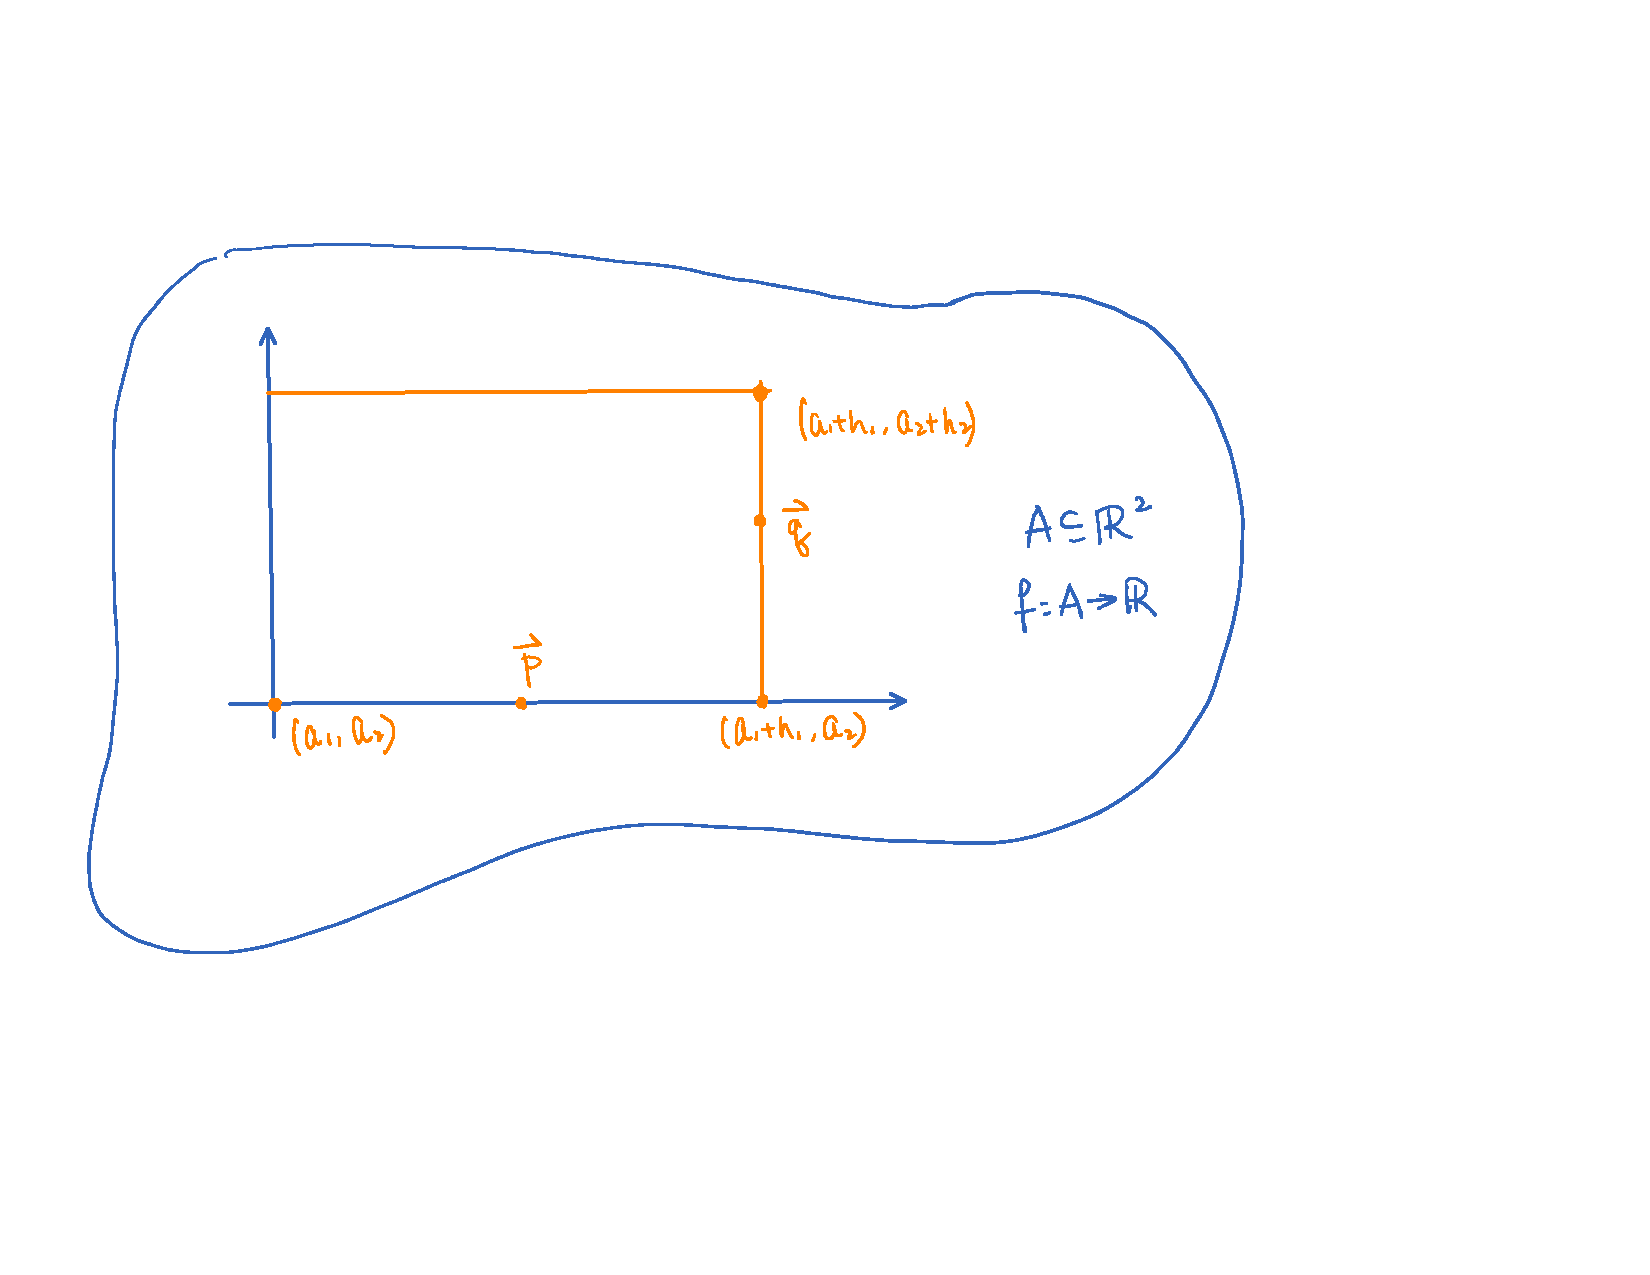
\includegraphics[scale=0.5]{thm6_1.pdf}
\end{center}
The proof for $m>2$ is left for reader, and can be found in Munkres Theorem 6.2.
\end{proof}

Suppose we have a continuous differentiable map from $A$ to $W$, where $A$ is a open subset of a vector space $V$ and $W$ is a vector space. Then we know that $Df:A \to B(V,W)$ is continuous, and $Df$ might be differentiable. If $Df$ is indeed differentiable, then we can define the following:
\begin{defn}
Let $V,W$ be vector spaces, let $A$ be an open subset of $V$, let $f:A \to W$ be a function that belongs to $C^1(A,W)$. We write $f \in C^2(A,W)$ provided that $Df\in C^1(A,B(V,W))$, that is, we write $f \in C^2(A,W)$ provided that $Df$ is differentiable at each $\vec{a}\in A$, and $D^2f$ is continuous on $A$, where $D^2f\coloneqq D(Df): A \to B(V,B(V,W))$
\end{defn}

\remark For vector spaces $V,W$\\ The set $B(V,B(V,W))$ can be viewed as a set of functions from $V \times V$ to $W$.\\

\note For vector spaces $\R^m,\R^n$, let $A$ be an open subset of $\R^m$, if $f:A \to \R^n\ \in C^2(A,\R^n)$, then $f\in C^1(A,\R^n)$ and each $D_{j_1}D_{j_2}f$ exists and is continuous on $A$, Theorem 6.1 provides the converse.

\begin{defn}
Let $V,W$ be vector spaces, let $A$ be an open subset of $V$,\\
$C^0(A,W) = C(A,W)$ is the set of continuous function from $A$ to $W$.
\end{defn}

\begin{defn}
Let $V,W$ be vector spaces, let $A$ be an open subset of $V$,\\
$$C^\infty(A,W) \coloneqq \bigcap_{r \in \N} C^r(A,W)$$
\end{defn}

\note For $r \in \N$, a function $f$ is of $C^r$ type if and only if $Df$  is of $C^{r-1}$ type.

\begin{thm}
Given $f\in C^2(A,\R)$, where $A$ is an open subset of $\R^2$. Then we can write the following: $$D_2D_1f(a,b) = \lim_{(h,k)\to (0,0)} \frac{f(a+h,b+k)-f(a+h,b)-f(a,b+k)+f(a,b)}{hk}$$
\end{thm}
\begin{proof}
Let $\phi:M\to \R \ \ \ s\mapsto f(s,b+k)-f(s,b)$ where $M$ is an open interval contained in $[a,a+h]$. Differentiate $\phi$ using the Chain Rule, then we can write $\phi'(s) = D_1f(s,b+k) - D_1f(s,b)$. $$\text{Let }num \coloneqq f(a+h,b+k)-f(a+h,b)-f(a,b+k)+f(a,b)$$ Using $\phi'(s) = D_1f(s,b+k) - D_1f(s,b)$, we can write: $$num = \phi(a+h)-\phi(a) = \phi'(s_0)\cdot h = (D_1f(s_0,b+k) - D_1f(s_0,b))\cdot h = D_2D_1f(s_0,t_0)\cdot k \cdot h$$ for some $s_0 \in [a,a+h]$ and $t_0 \in [b, b+k]$ by the Mean Value Theorem. For $\frac{num}{hk} = D_2D_1f(s_0,t_0)$, as $(h,k)$ tends to $(0,0)$, by continuity, we have $D_2D_1f(s_0,t_0)$ tends to $D_2D_1f(a,b)$, the result follows.
\begin{center}
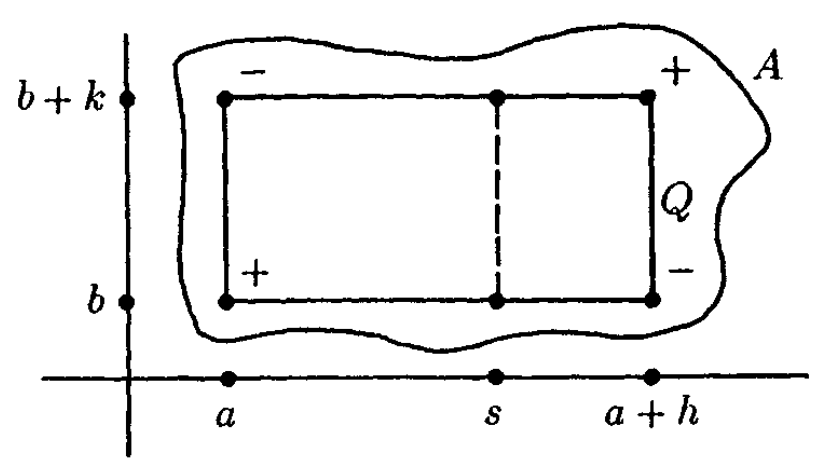
\includegraphics[scale=0.39]{thm6_2.png}${}$\ \ \  \\
(Figure 6.2 from Munkres Section 6)
\end{center}
\end{proof}

\note The existence of $D^2f$ is not enough for this result.\\

\begin{corT}[Clairaut's Theorem]
Given $f\in C^2(A,\R)$, where $A$ is an open subset of normed vector space $V$.\\ We have $D_1D_2f = D_2D_1f$
\end{corT}

\begin{defn}
Let $V,W$ be normed vector spaces, let $A$ be an open subset of $V$, let $f :A \to W$ be a function that is differentiable at $\vec{u}\in A$, we write  $D_{\vec{u}} f:A \to W\ \ \ \vec{a}\mapsto f'(\vec{a};\vec{u}) = (Df(\vec{a}))(\vec{u})$
\end{defn}

\begin{corT}
Given $f\in C^2(A,\R)$, where $A$ is an open subset of normed vector space $V$.\\ We have $D_{\vec{u}_1}D_{\vec{u}_2}f = D_{\vec{u}_2}D_{\vec{u}_1}f$
\end{corT}
\begin{proof}[Proof plan for Corollary 6.2.2]
Apply the Chain Rule to $(x_1,x_2) \mapsto f(\vec{a}+x_1\vec{u}_1+x_2\vec{u}_2)$
\end{proof}
\begin{proof}[Another proof plan for Corollary 6.2.2]
Adapt from the proof of Theorem 6.2, with the limit: $$\lim_{(h,k)\to (0,0)}\frac{f(\vec{a}+h\vec{u}_1+k\vec{u}_2)-f(\vec{a}+h\vec{u}_1)-f(\vec{a}+k\vec{u}_2)+f(\vec{a})}{hk} =D_{\vec{u}_1}D_{\vec{u}_2}f(\vec{a}) = D_{\vec{u}_2}D_{\vec{u}_1}f(\vec{a})$$
\end{proof}

\begin{corT}
Given $f\in C^2(A,\R^m)$, where $A$ is an open subset of normed vector space $V$.\\ We have $D_{\vec{u}_1}D_{\vec{u}_2}f = D_{\vec{u}_2}D_{\vec{u}_1}f$
\end{corT}
\begin{proof}
Apply the proof of Theorem 6.2 to each component function of $f$ and reassemble.
\end{proof}
\remark Theorem 6.2 and its corollaries also work for $f \in C^2(A,W)$ where $W$ is an arbitrary real normed vector space and $A$ is an open subset of $\R^2$. If $\dim W <\infty$, we can use the equivalence of norms to get the result similar to $W = \R^n$. If $\dim W = \infty$, the statements in the theorem and the corollaries are still true, but we need addition tools to prove.\\

Suppose $f\in C^r$, consider $D_{\vec{u}_1}\cdots D_{\vec{u}_r}f$
We can interchange $D\vec{u}_j$ with $D\vec{u}_{j+1}$ by Theorem 6.2 and its corollaries above, and hence any arbitrary permutation of $D\vec{u}_i$ can be achieved. \\

\exercise For $f \in C^r(\R^m,\R)$, find the number of distinct $D_{j_1},\cdots D_{j_r} f$.\\

\note For open set $A\subseteq \R^m$ and the function defined by the following: $$f =: A \to \R^n \ \ \ \vec{a}\mapsto  \begin{bmatrix} f_1(\vec{a})\\f_2(\vec{a})\\\vdots\\f_n (\vec{a})\end{bmatrix}$$ 
Here $f\in C^r(A,\R^n)$ if and only if for all $p\leq r$, $D_{j_1} D_{j_2}\cdots D_{j_p}f_r$ exists and is continuous. Also, for each of the $D_{j_1} D_{j_2}\cdots D_{j_p}f_r$, we can interchange the order of $D_{j_t}$ by the discussion above, and rewrite as $D_1^{\alpha_1}D_2^{\alpha_2}\cdots D_m^{\alpha_m}f_r$, where $\alpha_j \in \N\cup \{0\}$, $|\alpha| = \alpha_1+\alpha_2+\cdots +\alpha_m \leq r$. \\

\note Let $V,W$ be normed vector spaces, and let $A$ be an open subset of $V$, $B$ be an open subset of $W$. Suppose the function $f:A \to B$ is differentiable at $\vec{a}\in A$, and the function $g:B \to A$ is differentiable at $\vec{b} = f(\vec{a}) \in B$, with the property that $g\circ f = Id_A : A \to A \ \ \ \vec{x}\mapsto \vec{x}$. Then by the Chain Rule, we can write $Dg(\vec{b})\cdot Df(\vec{a}) = I$, where $I$ is the identity transformation, which implies $Dg(\vec{b})$ is a left inverse for $Df(\vec{a})$, and we must have $\dim(V) \leq \dim(W)$. Here, if we have $\dim(V) = \dim(W)< \infty$, then  it is immediate that $Dg(\vec{b})$ is a two-sided inverse for $Df(\vec{a})$. Or, if we have $f\circ g = Id_B: B \to B \ \ \ \vec{y}\mapsto \vec{y}$. Then $Dg(\vec{b})$ will also become a two-sided inverse for $Df(\vec{a})$, and we have $\dim(V) = \dim(W)$.\\

\begin{prop}
Let $V,W$ be normed vector spaces with $\dim(V)<\infty$ and $\dim(W) < \infty$, and let $A$ be an open subset of $V$, $B$ be an open subset of $W$. Suppose $f:A \to B$ and $g:B \to A$ are continuous, not necessarily differentiable, with the property that $g\circ f = Id_A$ and $f\circ g = Id_B$, then we have $\dim(V) = \dim(W)$.
\end{prop}
\hfill [L. E. J. Brouwer, 1912]\\
\hfill\break

\exercise There exists a continuous surjection from $\R$ to $\R^2$.\\

\newpage
\section[Homeomorphism and Diffeomorphism]{\color{red} Homeomorphism and Diffeomorphism \color{black}}

\begin{defn}
A homeomorphism is a continuous bijective function $f$ whose inverse is also continuous. 
\end{defn} 

\example Let $S^1\coloneqq\{(x,y) \in\R^2 \mid x^2 + y^2 = 1\}$.\\
Consider the function $f:[0,2\pi) \to S^1 \ \ \ t\mapsto (\cos(t),\sin(t))$. Notice here $f$ is a bijection, but not a homeomorphism from $[0,2\pi)$ to $S$. This can be shown by considering the sequence $(a_n)$, where $a_i = (\cos(1/i),-\sin(1/i))$. $(a_n)$ converges to $(1,0)$. The sequence $(f^{-1}(a_n))$ converges to $2\pi$, but we have $f^{-1}(-1,0) = 0$, hence $f^{-1}$ is not continuous.

\begin{defn}
Let $A$ be an open subset of normed vector space $V$ and let $B$ be an open subset of normed vector space $W$. A function $f:A \to B$ is called a $C^r$-diffeomorphism provided that $f$ is a bijection, $f\in C^r(A,B)$, and $f^{-1} \in C^r(B,A)$.
\end{defn}

\example $f:\R \to \R \ \ \ t\mapsto t^3$ is a homeomorphism, but not a $C^r$-diffeomorphism. 

\begin{defn}
A complete normed vector space is called a Banach space.
\end{defn}


\example Consider the set $A = \left\{\begin{bmatrix} r\\\theta \end{bmatrix} \in \R^2 \mid r>0\right\}$. Let $f:A \to \R^2 \ \ \ \begin{bmatrix} r\\\theta \end{bmatrix}\mapsto \begin{bmatrix} r\cos(\theta)\\r\sin(\theta )\end{bmatrix}$.\\ Here we note that $f$ is of $C^\infty$ type, and we can write the following: $$Df\left(\begin{bmatrix} r\\\theta \end{bmatrix}\right) = \begin{bmatrix} \cos\left(\theta\right)& -r\sin\left(\theta\right)\\\sin\left(\theta\right)&r\cos\left(\theta\right) \end{bmatrix}$$
where we have: $$\det\left(Df\left(\begin{bmatrix} r\\\theta \end{bmatrix}\right)\right) = r$$ here we know that $Df\left(\begin{bmatrix} r\\\theta \end{bmatrix}\right)$ is invertible for all $\begin{bmatrix} r\\\theta \end{bmatrix} \in A$, but $f$ is not injective on $A$. \\Note that $f\left(A\right) = \R^2 \setminus \{0\}$, and there exists local $C^\infty$ inverse for $f$, but not global inverse.

\begin{defn}
Let $A,B$ be topological spaces, a function $f:A \to B$ is said to be open proved that $f(U)$ is open in $B$ when $U$ is open in $A$.
\end{defn}

\note If a function $f$ is a bijection.
\begin{enumerate}[topsep=3pt,itemsep=-1ex,partopsep=1ex,parsep=1ex]
\item $f$ is continuous if and only if $f^{-1}$ is open.
\item $f$ is open if and only if $f^{-1}$ is continuous.
\item $f$ is a homeomorphism if and only if $f$ is continuous and open.\\
\end{enumerate}

\begin{thm}[\color{red}Inverse Function Theorem\color{black}]
Let $A $ be an open subset of $\R^n$, let $\vec{a}\in A$, let $f\in C^r(A,\R^n)$ with $r\geq 1$, and given $Df(\vec{a})$ is invertible. There exists an open neighborhood $U$ of $\vec{a}$ such that $f|_U$ is a $C^r$-diffeomorphism, that is, $f$ maps $U$ bijectively to some open set in $\R^n$, and $f^{-1}:f(U) \to U$ is of $C^r$ type. 
\end{thm}
\note $E = \{ \vec{x}\in A\mid Df(\vec{x})$ is invertible $\} = \{\vec{x}\in A \mid \det(Df(\vec{x})) \neq 0\}$ is an open set containing $\vec{a}$. 

\note The theorem does not assume that $E=A$, but we could assume such by replacing $A$ by $E$.

\begin{proof}[Proof of the Inverse Function Theorem]
\hfill\break First we need some preliminaries:\begin{enumerate}[topsep=3pt,itemsep=-1ex,partopsep=1ex,parsep=1ex]
\item Let $T_{\vec{a}}$ be a function such that $\vec{x} \mapsto \vec{x}+\vec{a}$
\item Let $g$ denote the function $Df(\vec{a})^{-1}\circ T_{-f(\vec{a})} \circ f\circ T_{\vec{a}}$
\end{enumerate}

From (2), we note that the following holds:
\begin{enumerate}[topsep=3pt,itemsep=-1ex,partopsep=1ex,parsep=1ex]
\item $g(\vec{0}) = \vec{0}$
\item $Dg(\vec{0}) = I$ where $I$ is the identity transformation
\item $f = T_{f(\vec{a})}\circ Df(\vec{a})\circ g\circ T_{-\vec{a}}$
\end{enumerate}

In the following, diffeomorphism refers to $C^r$-diffeomorphism. It suffices to show that $g$ is a diffeomorphism on some open set containing $\vec{0}$. First we let $h = g-Id$, then we know that $Dh = Dg-I$, and $Dh(\vec{0}) = 0$, which implies that each $D_j h_k(\vec{0}) = 0$, $\forall 1\leq j,k \leq n$. Fix $\mu >0$, then there exists $\delta >0$ such that for $\vec{x}\in B_\delta(\vec{0})$, we have each $|D_jh_k(\vec{x})| < \mu$. Let $\vec{x} \in B_\delta(\vec{0})$, consider $Dh(\vec{x})(\vec{u})$. 
$$Dh(\vec{x})(\vec{u}) = \begin{bmatrix}
\sum_j D_jh_1(\vec{x})u_j\\\sum_j D_jh_2(\vec{x})u_j \\ \vdots \\ \sum_j D_j h_n (\vec{x})u_j
\end{bmatrix}$$

$$||Dh(\vec{x})(\vec{u})||= \left|\left|\begin{bmatrix}
\sum_j D_jh_1(\vec{x})u_j \\ \vdots \\ \sum_j D_j h_n (\vec{x})u_j
\end{bmatrix}\right|\right|\leq \sqrt{n} \left|\begin{bmatrix}
\sum_j D_jh_1(\vec{x})u_j \\ \vdots \\ \sum_j D_j h_n (\vec{x})u_j
\end{bmatrix}\right| \leq \sqrt{n}n\cdot \mu |\vec{u}|\leq n^\frac{3}{2}\mu ||\vec{u}||$$
which implies the following holds:
$$||Dh(\vec{x})|| \leq n^{\frac{3}{2}} \mu \qquad\qquad\qquad\text{for }\vec{x} \in B_\epsilon(\vec{0})$$
Fix $0 <\epsilon <1$, let $\mu = \frac{\epsilon}{n^{3/2}}$, then by previous argument, there exists $\delta>0$ such that $\forall \vec{x}\in B_\delta(\vec{0})$, we have $||Dh(\vec{x})||<n^{3/2}\mu = \epsilon$. By using Lipschitz Estimate from Math 395 HW4, we get that $||h(\vec{x}) -h(\vec{y})|| \leq \epsilon ||\vec{x}-\vec{y}||$ for $\vec{x},\vec{y}\in B_\delta(\vec{0})$. Then for $\vec{x},\vec{y}\in B_\delta(\vec{0})$, we have: $$||g(\vec{x})-g(\vec{y})|| = ||\vec{x}-\vec{y} +h(\vec{x})-h(\vec{y})||\leq ||\vec{x}-\vec{y}|| + ||h(\vec{x}) - h(\vec{y})|| \leq (1+\epsilon) ||\vec{x}-\vec{y}||$$
Also, we have the following by the reverse triangle inequality:
$$||g(\vec{x})-g(\vec{y})|| = ||\vec{x}-\vec{y}+h(\vec{x})-h(\vec{y})|| \geq ||\vec{x}-\vec{y}|| - ||h(\vec{x})-h(\vec{y})|| \geq (1-\epsilon)||\vec{x}-\vec{y}||$$
because we have $0< \epsilon<1$, here we see that $g$ is injective on $B_\delta(\vec{0})$.\\ 
Here $B_\delta(\vec{0})$ is a convex set. Let $\psi_y : \vec{x}\mapsto \vec{y}-h(\vec{x})$.\\ Pick $0 < \widetilde{\delta} < \delta$ such that for $\vec{y}\in B_{(1-\epsilon)\widetilde{\delta}}(\vec{0})$ and $\vec{x}\in \overline{B_{\widetilde{\delta}}(\vec{0})}$, we have: $$||\psi_y(\vec{x})|| \leq (1-\epsilon)\widetilde{\delta} + \epsilon\widetilde{\delta} = \widetilde{\delta}$$
so the function $\psi_y:\overline{B_{\widetilde{\delta}}(\vec{0})} \to \overline{B_{\widetilde{\delta}}(\vec{0})}$ is well defined, with the following holds:
$$||\psi_y(\vec{x}_1) - \psi_y(\vec{x}_2) || \leq ||h(\vec{x}_2)-h(\vec{x}_1)|| \leq \epsilon||\vec{x}_2-\vec{x}_1||$$
So $\psi_y$ is a contraction on $\overline{B_{\widetilde{\delta}}(\vec{0})}$ where $\overline{B_{\widetilde{\delta}}(\vec{0})}$ is a complete metric space. By the Contraction Mapping Theorem, there exists a unique $\vec{x}\in \overline{B_{\widetilde{\delta}}(\vec{0})}$ such that $\psi_y(\vec{x})= \vec{y}-h(\vec{x}) = \vec{x}$, that is, $g(\vec{x}) = \vec{y}$. Take unions $\bigcup_{\widetilde{\delta} < \delta}\overline{B_{\widetilde{\delta}}(\vec{0})} = B_\delta(\vec{0})$ and $\bigcup_{\widetilde{\delta} < \delta}B_{(1-\epsilon)\widetilde{\delta}}(\vec{0}) = B_{(1-\epsilon)\delta}(\vec{0})$ to get $B_{(1-\epsilon)\delta}(\vec{0}) \subseteq g(B_{\delta}(\vec{0}))\subseteq g(A)$. Notice we get $\vec{0} \in $Int$(g(A))$. \\

We conclude the results that we shown above as a lemma:

\begin{lem}
\setlength{\leftskip}{1cm} Let $A$ be an open subset of $\R^n$, let $\vec{a}\in A$, let $f\in C^r(A,\R^n)$ with $r\geq 1$, and given $Df(\vec{a})$ is invertible. Let $T_{\vec{a}}$ be a function that maps $\vec{x}$ in its domain to $\vec{x}+\vec{a}$ in its codomian, with some $\vec{a}$ in its domain. Let $g$ denote the function $Df(\vec{a})^{-1}\circ T_{-f(\vec{a})} \circ f\circ T_{\vec{a}}$, and let $h = g-Id$ where $Id$ is the identity function. We have the followings hold:
\begin{enumerate}[topsep=3pt,itemsep=-1ex,partopsep=1ex,parsep=1ex,leftmargin=1.5cm]
\item For $\mu>0$, there exists $\delta>0$ such that for all $\vec{x}\in B_\delta(\vec{0})$, we have $||Dh(\vec{x})||\leq n^{3/2}\mu$.
\item For $0<\epsilon<1$, $\exists\ \delta>0$ s.t. $\forall \vec{x},\vec{y}\in B_\delta(\vec{0})$, $||h(\vec{x})-h(\vec{y})|| \leq \epsilon ||\vec{x}-\vec{y}||$
\item For $0<\epsilon<1$, $\exists\ \delta>0$ s.t. $\forall  \vec{x},\vec{y}\in B_\delta(\vec{0})$, $(1-\epsilon)||\vec{x}-\vec{y}|| \leq ||g(\vec{x})-g(\vec{y})|| \leq (1+\epsilon)||\vec{x}+\vec{y}||$
\item For $0<\epsilon<1$, $\exists\ \delta>0$ s.t. $g$ is injective on $B_{\delta}(\vec{0})$.
\item For $0<\epsilon<1$, $\exists\ \delta>0$ s.t. $B_{(1-\epsilon)\delta}(\vec{0}) \subseteq g(B_{\delta}(\vec{0}))\subseteq g(A)$.
\item $\vec{0}\in $ Int\,$(g(A))$.
\end{enumerate}
\end{lem}

To proceed proving the Inverse Function Theorem, we will make use of the following Theorem:

\begin{thm}
\setlength{\leftskip}{1cm} Given $E$ as a open subset of $\R^n$, $f \in C^1(E,\R^n)$, and $\det(Df(\vec{x})) \neq 0$ for all $\vec{x}\in E$. \\Then we have the followings hold:
\begin{enumerate}[topsep=3pt,itemsep=-1ex,partopsep=1ex,parsep=1ex,leftmargin=1.5cm]
\item $\vec{a}\in E$ implies $f(\vec{a}) \in $ Int\,$(f(E))$.
\item $f(E)$ is open in $\R^n$.
\item $f:E \to f(E)$ is an open map.
\end{enumerate}
\end{thm}

\begin{proof}[Proof of Theorem 7.2]
\setlength{\leftskip}{1cm} Fix $\vec{a}\in E$, apply Lemma 7.1.1 to $g = Df(\vec{a})^{-1} \circ T_{-f(\vec{a})}\circ f \circ T_{\vec{a}}$ defined on the set $T_{-\vec{a}}(E)$. Notice here $g(\vec{0}) = \vec{0}$, and $Dg(\vec{0}) = I$, and we have $\vec{0}\in $Int$($Im$(g))$. Consider $Df(\vec{a})\circ g$, we see that $\vec{0}\in $\,Int$($Im$(Df(\vec{a})\circ g))=$\,Int\,$($Im$(T_{-f(\vec{a})}\circ f\circ T_{\vec{a}}))$. Then we consider $T_{f(\vec{a})}\circ Df(\vec{a})\circ g$, we have $f(\vec{a})\in$Int$($Im$(f\circ T_{\vec{a}}))=$Int$(f(E))$, which implies (1) holds, and (2) follows immediately as $f(E)$ contains all its interior points. For (3), let $U$ be an open subset of $E$, apply (2) to $f|_U$ and the result follows.
\end{proof}

\begin{corT}
\setlength{\leftskip}{1cm} Given $E$ as a open subset of $\R^n$, $f \in C^1(E,\R^n)$, and $\det(Df(\vec{x})) \neq 0$ for all $\vec{x}\in E$.\\ If $f$ is injective, then $f:E \to f(E)$ is a homeomorphism.
\end{corT}


Using Lemma 7.1.1, we know that for $0<\epsilon<1$, $\exists\ \delta>0$ such that $g$ is injective on $B_{\delta}(\vec{0})$. Since $Df(\vec{a})$ is invertible, then $Df(\vec{a})$ is injective. So we know that the composition of injective functions $f|_{B_{\delta}(\vec{a})}=T_{f(\vec{a})} \circ Df(\vec{a}) \circ g|_{B_{\delta}(\vec{0})} \circ T_{-\vec{a}}$ is injective, then by Corollary 7.2.1, let $U = E \cap B_{\delta}(\vec{a})$, where $E$ is the open neighborhood of $\vec{a}$ in which $\det(Df(\vec{t})) \neq 0$ for all $\vec{t}\in E$, then we know that $f|_U: U\to f(U)$ defines a homeomorphism. On the other hand, we know that for all $\vec{x},\vec{y} \in U = B_\delta(\vec{0})$, we have $(1-\epsilon)||\vec{x}-\vec{y}|| \leq ||g(\vec{x}) - g(\vec{y}) || \leq (1+\epsilon) ||\vec{x}+\vec{y}||$, so we know that $g$ is bi-Lipschitz from $B_{\delta}(\vec{0})$ to $g(B_{\delta}(\vec{0}))$. It follows that $f|_U$ is bi-Lipschitz as the composition of bi-Lipschitz functions is bi-Lipschitz. To show that $f|_U$ is a diffeomorphism, we will make use of the following Proposition:


\begin{prop}
\setlength{\leftskip}{1cm} Given $E$ as a open subset of $\R^n$, $f \in C^1(E,\R^n)$ is an injective function, with $\det(Df(\vec{x})) \neq 0$ for all $\vec{x}\in E$. Then we have $f \in C^r$ implies $f^{-1} \in C^r$. 
\end{prop}
\begin{proof}
\setlength{\leftskip}{1cm}It suffices to show that $\psi \coloneqq f^{-1}$ is $C^1$. Fix $\vec{a}\in E$. Let $\vec{b} \in f(\vec{a})$, and let $M\coloneqq Df(\vec{a})$. To show that $\psi$ is differentiable, we want to find some $T$ such that the following holds:
\begin{align*}\lim_{\vec{k}\to \vec{0}}\frac{\psi(\vec{b}+\vec{k})-\psi(\vec{b}) - T\vec{k}}{||\vec{k}||} = 0 \tag{1}
\end{align*}
Let $T = M^{-1}$, $\vec{h}= \psi(\vec{b}-\vec{k})-\psi(\vec{b})$, then we can write the following:
\begin{align*}
\frac{\psi(\vec{b}+\vec{k})-\psi(\vec{b}) - M^{-1}\vec{k}}{||\vec{k}||} &= \frac{\vec{h}-M^{-1}\vec{k}}{||\vec{k}||}\\ &= -M^{-1}\left(\frac{\vec{k}-M\vec{h}}{||\vec{k}||}  \right)\\
&= -M^{-1} \left(\frac{f(\vec{a}+\vec{h}) - f(\vec{a}) - M\vec{h}}{||\vec{h}||}  \right)\left(\frac{||\vec{h}||}{||\vec{k}||} \right) \\
&\coloneqq -M^{-1} (*)(**)
\end{align*}
where $(**)$ is bounded for small $||\vec{k}||$ by Lemma 7.1.1 (3), and we have $\vec{h}\to \vec{0}$ as $\vec{k}\to \vec{0}$. While $(*)$ tends to $0$ as $f$ is differentiable, we know that equation (1) must hold. Now we have shown that $\psi$ is differentiable and we have $D\psi(\vec{b}) = [Df(\psi(\vec{b}))]^{-1}$. Lastly, we will show that $D\psi: f(E) \to $Mat$(n,n,\R)$ is continuous. Here we have the following holds:
$$f(E)\xrightarrow[continuous]{\psi}E\xrightarrow[continuous]{Df}GL_{n}(\R) \xrightarrow[continuous]{Inverse}GL_{n}(\R)$$
with $D\psi = Inverse \circ Df \circ \phi$, here $Inverse$ is the function that sends an invertible matrix $M\in GL_{n}(\R)$ to its inverse $M^{-1}\in GL_{n}(\R)$. $Inverse$ is a continuous function by Cramer's Rule and Theorem 2.14 on Munkres. We know that the composition of continuous functions is continuous, hence $D\psi$ is continuous. This finishes the proof for $r=1$. For $r>1$, we can proceed by induction. Assume the result is known for $C^{r-1}$, where $\psi$ and $Df$ are of $C^{r-1}$ type, and we know that $C^{r-1}$ is closed under composition, then the result follows immediately. 
\end{proof}

Here we see that the results for the Inverse Function Theorem follows from Proposition 7.2.2 and Corollary 7.2.1. This completes the proof for the Inverse Function Theorem. \end{proof}
\hfill\break\hfill\break

For $V,W,Z$ be normed vector spaces, and let $A$ be a open subset of $V$, $B$ be a subset of $W$. Consider function $f:A \to B$ and $g:B \to Z$, then we can write the chain rule $D(g\circ f) = ((Dg)\circ f) \circ Df$. If we have stronger condition where $f,g \in C^1$, then $Dg,f,Df$ are all continuous, hence we know that the composition of continuous functions $D(g\circ f)\in C^1$. If we have $f \in C^2$, then $D^2f:A \to B(V,B(V,W))$.
Now suppose $f,g \in C^2$, then $Df,Dg\in C^1$, and hence $D(g\circ f) \in C^1$ by the Chain Rule and composition of $C^1$ function, we have $g\circ f \in C^2$. \\ 

\note Consider an affine function $f$ which sends $\vec{x}$ to $T\vec{x}+b$, where $T$ is a linear transformation. We have $Df(\vec{x}) = T$, and $D^2f(\vec{x})=0$, because $T$ is a "constant" in the space $B(V,W)$.  \\

Let $V$ be a normed vector space, and let $A$ be an open subset of $V$.\\
\exercise Let $f,g \in C^r(A,\R)$, then we have $g\circ f \in C^r$.\\
\exercise Let $f \in C^r(A,\R\setminus\{0\})$, then we have $\frac{1}{f}\in C^r$.\\
\exercise Let $f,g \in C^r(A,\R)$, then we have $f+g \in C^r$, and $fg \in C^r$.\\


\blfootnote{This page number is Jinyan's favorite number}

\newpage
\textbf{Leibniz's Notation in Several Variables}\\
Suppose we have five quantities, $x,y,u,v,t$, such that any two of these variables determine the other three. Consider the following:
$$f:\begin{bmatrix}
x\\y \end{bmatrix} \mapsto \begin{bmatrix}
u\\v \end{bmatrix}
$$
where we define
$$\begin{bmatrix}
\frac{\partial u}{\partial x} &\frac{\partial u}{\partial y} \\
\frac{\partial v}{\partial x} &\frac{\partial v}{\partial y}
\end{bmatrix} \coloneqq 
Df = \begin{bmatrix}
D_1f_1 & D_2f_2 \\ D_1f_2 & D_2f_2
\end{bmatrix} 
$$
Consider another function defined by the following:
$$g:
\begin{bmatrix}
u\\v
\end{bmatrix}\mapsto t$$
and we define:
$$
\begin{bmatrix}
\frac{\partial t}{\partial u}& \frac{\partial t}{\partial v}
\end{bmatrix} \coloneqq
Dg = \begin{bmatrix}D_1g& D_2g
\end{bmatrix}
$$
Then we write the following:
\begin{align*}
\begin{bmatrix}
\frac{\partial t}{\partial x} & \frac{\partial t}{\partial y}
\end{bmatrix} = D(g\circ f) = (Dg\circ f)\circ Df 
= \begin{bmatrix}
\frac{\partial t}{\partial u}& \frac{\partial t}{\partial v}
\end{bmatrix} \begin{bmatrix}
\frac{\partial u}{\partial x}&\frac{\partial u}{\partial y}\\
\frac{\partial v}{\partial x}&\frac{\partial v}{\partial y}
\end{bmatrix}
=
\begin{bmatrix}
\frac{\partial t}{\partial u}\frac{\partial u}{\partial x}+\frac{\partial t}{\partial v}\frac{\partial v}{\partial x}& \frac{\partial t}{\partial u}\frac{\partial u}{\partial y} + \frac{\partial t}{\partial v}\frac{\partial v}{\partial y}
\end{bmatrix}
\end{align*}
Notice here, one disadvantage of using the Leibniz's Notation is that the notation "$\frac{\partial t}{\partial u}$" does not specify what quantity is being held "fixed" when taking the derivative. \\







\newpage
\section[Implicit Function Theorem]{\color{red} Implicit Function Theorem \color{black}}
Consider $M \in $Mat$(n,k+n,\R)$, $\vec{c}\in \R^n$, let $E=\{ \vec{v}\in \R^{k+n} \mid M\vec{v} = \vec{c}\}=\{ \vec{v}\in \R^{k+n} \mid M\vec{v}- \vec{c}=\vec{0}\}$. Now define $T:\R^{k+n} \to \R^{n} \ \ \ \vec{v}\mapsto M\vec{v}-\vec{c}$. Here $T$ is an affine.  Let $\hat{M}: \R^{k+n} \to \R^n \ \ \ \vec{v}\mapsto M\vec{v}$. Note here $E$ could be empty, if $E$ is non-empty, then $E $ is an affine set because $E=\ker(\hat{M})+\vec{v}_p$ where $\vec{v}_p$ is any particular solution of $M\vec{v}_p = \vec{c}$. We also have $\dim(E) = \dim(\ker(\hat{M})) = k+n - \text{rank}(M)$ by the Rank-Nullity Theorem. Here we have $k \leq \dim(E) \leq k+n$. \\

In the following discussion, we will investigate if we can write $E$ as Graph$(g)$ for some $g:\R^k \to \R^n$. If such is true, then $g$ has to be affine. Consider the following:
$$M=\begin{bmatrix}
X & Y
\end{bmatrix}\text{ where }X\text{ is an }n\times k\text{ matrix, and } Y \text{ is an }n\times n\text{ matrix}$$
For $\vec{x}\in \R^k$ and $\vec{y}\in \R^n$, we can write the following:
\begin{align*}
M\begin{bmatrix}
\vec{x}\\\vec{y}
\end{bmatrix} = X\vec{x} + Y\vec{y}
\end{align*}

Case (1): $Y$ is non-invertible, then there exists $\vec{w}\in \R^n$ such that $Y\vec{w} = \vec{0}$ with $\vec{w}\neq \vec{0}$.\\ Then for $(\vec{x},\vec{y}) \in E$, we have the following holds:
\begin{align*}
\begin{bmatrix}
\vec{x}\\\vec{y}
\end{bmatrix} \in E \qquad\Rightarrow \qquad \begin{bmatrix}
\vec{x}\\\vec{y}+\vec{w}
\end{bmatrix} \in E
\end{align*}

Case (2): $Y$ is invertible, then we have the following holds:
\begin{align*}
M\begin{bmatrix}
\vec{x}\\\vec{y}
\end{bmatrix} = \vec{c} \iff Y^{-1}X\vec{x} + \vec{y} = Y^{-1}\vec{c} \iff \vec{y} = -Y^{-1}X\vec{x}+ Y^{-1}\vec{c} \coloneqq T(\vec{x})
\end{align*}
Here we see that $T$ is an affine function.\\

Consider $Proj_{k+1,\cdots,n} = [Z\ I]$ where $Z$ is an $n \times k$ zero matrix and $I$ is an $n \times n$ identity matrix. $$\hat{Proj_{k+1,\cdots,n}}:\R^{k+n} \to \R^n \ \ \ \begin{bmatrix}\vec{x}\\\vec{y}\end{bmatrix} \mapsto \vec{y}$$
Note here we have $Y = Proj_{k+1,\cdots,n}\cdot M$.\\

Here, one might want a different set of $k$ independent vectors on the graph.\\ Let $\hat{p}: \R^{k+n} \to \R^{k+n} \ \ \ \vec{x}\mapsto P\vec{x}$ be a coordinate permutation, where we have: 
$$P = \begin{bmatrix}
 \vec{e}_{j_1} \\ \vec{e}_{j_2} \\ \vdots \\ \vec{e}_{j_{k+n}}
\end{bmatrix}$$
here we view each standard basis vector $\vec{e}_{j_i}$ as a row vector.\\
The image $\hat{p}($Graph$(g))$ is a coordinate permuted graph with $k$ independent variables. 
\begin{align*}
\dim(E) = k &\iff \text{rank}(M) = n \iff \text{some }n\times n\text{ submatrix of }M\text{ is invertible}\\
&\iff E\text{ is permuted graph of an affine function with k independent variables}
\end{align*}

Consider a general vector in $\R^{k+n}$ defined by the following:
$$\vec{G} = \begin{bmatrix}
\vec{x} \\ \vec{y}
\end{bmatrix}\qquad\qquad\qquad\vec{x}\in \R^k,\ \vec{y}\in \R^n
$$
and a special vector in $\R^{k+n}$ defined by the following:
$$\vec{S} = \begin{bmatrix}
\vec{a} \\ \vec{b}
\end{bmatrix}\qquad\qquad\qquad\vec{a}\in \R^k,\ \vec{b}\in \R^n
$$
The Implicit Function Theorem states that, for $f \in C^r(A,\R^n)$, where $A$ is an open subset of $\R^{k+n}$, and given that the following holds:
\begin{align*}
\begin{bmatrix}
\vec{a}\\\vec{b}
\end{bmatrix} \in f^{-1}(\vec{0}) \coloneqq E \qquad\qquad\qquad \frac{\partial f}{\partial \vec{y}}\begin{bmatrix}
\vec{a}\\\vec{b}
\end{bmatrix} \text{ is invertible}
\end{align*}

Then there exists an open neighborhood $U$ of $\vec{S}$ such that $E \cap U = $Graph$(g)$ for some $g \in C^r(B,\R^n)$ where we have $\vec{a}\in B$ and $B$ is an open subset of $\R^k$. That is, we can solve for $\vec{y}$ in terms of $\vec{x}$ near $\vec{S}$. \\


\newpage
\begin{thm}[Implicit Function Theorem]
Let $\vec{G}$ in $\R^{k+n}$ defined by the following:
$$\vec{G} = \begin{bmatrix}
\vec{x} \\ \vec{y}
\end{bmatrix}\qquad\qquad\qquad\vec{x}\in \R^k,\ \vec{y}\in \R^n
$$
and fix $\vec{S}$ in $\R^{k+n}$ by the following:
$$\vec{S} = \begin{bmatrix}
\vec{a} \\ \vec{b}
\end{bmatrix}\qquad\qquad\qquad\vec{a}\in \R^k,\ \vec{b}\in \R^n
$$
For $f \in C^r(A,\R^n)$, where $A$ is an open subset of $\R^{k+n}$. If we have the followings hold:
\begin{align*}
\vec{S} \in f^{-1}(\vec{0}) \coloneqq E \qquad\qquad\qquad \left[\frac{\partial f}{\partial \vec{y}}\ \vec{S}\right] \text{ is invertible}
\end{align*}

Then there exists a neighborhood $U$ of $\vec{S}$ such that $E \cap U = $Graph$(g)$ for a unique function $g \in C^r(B,\R^n)$, where $\vec{a}\in B$, and $B$ is an open subset of $\R^k$. In other words, $\exists$ an open neighborhood $B$ of $\vec{x}$ such that $\vec{y} = g(\vec{x})$ and $f(\vec{x},g(\vec{x})) = \vec{0}$ for all $\vec{x}\in B$, with a unique function $g \in C^r(B,\R^n)$.
\end{thm}


\begin{proof}
We will construct a function $F$ to which we can apply the Inverse Function Theorem: $$F:A \to \R^{k+n}\qquad\qquad \begin{bmatrix}
\vec{x}\\\vec{y}
\end{bmatrix} \mapsto \begin{bmatrix}
\vec{x}\\ f\begin{bmatrix}
\vec{x}\\\vec{y}
\end{bmatrix}
\end{bmatrix} \text{\ \ \  for }\vec{x}\in \R^k,\ \vec{y}\in \R^n$$ 

Here we note that $f\begin{bmatrix} \vec{x}\\\vec{y} \end{bmatrix} \in \R^n$, and $F \in C^r(A,\R^{k+n})$ with:
$$DF = \begin{bmatrix}
I & Z \\ 
\frac{\partial f}{\partial \vec{x}}& \frac{\partial f }{\partial \vec{y}}
\end{bmatrix}$$

Here $I$ is the ${k \times k}$ identity matrix, $Z$ is the ${k \times n}$ zero matrix. $\frac{\partial f}{\partial \vec{x}}$ is an ${n \times k}$ matrix, and $\frac{\partial f }{\partial \vec{y}}$ is an ${n \times n}$ matrix. Note that $DF = \det I \cdot \det \frac{\partial f}{\partial \vec{y}} \neq 0$ by Munkres Lemma 2.12. Hence we know that the $DF$ is invertible when evaluated at $\vec{S}$. Here the inverse of $DF$ is given by the following:
$$(DF)^{-1} = \begin{bmatrix}
I & Z \\ -\left(\frac{\partial f}{\partial \vec{x}}\right)^{-1}\frac{\partial f}{\partial \vec{x}} & \left(\frac{\partial f}{\partial \vec{y}}\right)^{-1}
\end{bmatrix}$$
By the Inverse Function Theorem, we know that $F$ has local inverse of $C^{1}$ type, then we can write the following with a function $h$ of $C^r$ mapping an open set $U\subseteq \R^{k+n}$ to $R^n$:
$$F^{-1}: W \to \R^n \qquad \begin{bmatrix}
\vec{x}\\\vec{z}
\end{bmatrix}  \mapsto \begin{bmatrix}
\vec{x} \\ h\begin{bmatrix}
\vec{x} \\ \vec{z}
\end{bmatrix}
\end{bmatrix} \text{\ \ \  for }\vec{x}\in \R^k,\ \vec{z}\in \R^n$$
Near $\vec{S}$, we have the following holds:
\begin{align*}
\begin{bmatrix}
\vec{x}\\\vec{y}
\end{bmatrix}\in E \iff f\begin{bmatrix}
\vec{x}\\\vec{y}
\end{bmatrix} = \vec{0} \iff F\begin{bmatrix}
\vec{x}\\ \vec{y}
\end{bmatrix}  =\begin{bmatrix}
\vec{x} \\ \vec{0}
\end{bmatrix} &\iff \begin{bmatrix}
\vec{x}\\\vec{y}
\end{bmatrix} = F^{-1}\begin{bmatrix}
\vec{x}\\ \vec{0}
\end{bmatrix}=\begin{bmatrix}
\vec{x} \\ h\begin{bmatrix}
\vec{x} \\ \vec{0}
\end{bmatrix}
\end{bmatrix}  \\&\iff \vec{y} = h\begin{bmatrix}
\vec{x}\\\vec{0}
\end{bmatrix}\coloneqq g(\vec{x})
\end{align*}
One can show that $g$ is unique and the result follows. 
\end{proof}
More details of this proof can be found on Munkres Theorem 9.2.
\hfill\break

In the proof of the Implicit Function Theorem:\\
\remark $F$ gives "change of coordinates" that locally straightens all levels set of $f$. 

\remark $E$ is locally a coordinate permuted graph if rank$(Df(\vec{S}))= n$.


\newpage
\section[Optimization]{\color{red} Optimization \color{black}}

\begin{thm}[First Derivative Test for Higher Dimensions]
Let $\Omega$ be an open subset of $\R^n$, and let $h: \Omega \to \R$ be a function that achieves a local maximum, or minimum, at $\vec{p}\in \Omega$, then $Dh(\vec{p}) = 0$.
\end{thm}
\begin{proof}
Suppose we have $h \in C^1(\Omega, \R)$ where $\Omega$ is an open subset of $\R^n$, with the property that $h$ achieves a maximum, or a minimum, at $\vec{p}\in \Omega$. Consider arbitrary $\gamma \in C^1(A, \Omega)$ with $\gamma(0) = \vec{p}$, where $A$ is an open subset of $\R$. Then $h\circ \gamma$ has a maximum, or a minimum, at $t=0$. So we have $0 = (h \circ \gamma)' (0) = Dh(\gamma(0))\gamma'(0)$. Since this is true for arbitrary $\gamma$ that satisfies $\gamma(0) = \vec{p}$, here we can conclude that $Dh(\gamma(0))=Dh(\vec{p}) = \vec{0}$, and hence we can write: 
$$D_1h(\vec{p}) = D_2h(\vec{p}) = \cdots  = D_nh(\vec{p}) = 0$$

Now assume $h$ has global maximum, or global minimum, at $\vec{p}$. Then for an open subset $U$ that contains $\vec{p}$, $h|_U$ has a local maximum, or a local minimum, and we can reach the same conclusion that $Dh(\vec{p}) = \vec{0}$ with the same argument. That is, $Dh(\vec{p}) = 0$ holds true regardless whether the maximum, or minimum, is global or local.
\end{proof}


\begin{thm}[Lagrange Multiplier Theorem]
Let $U$ be an open subset of $\R^{k+n}$, let the constraint function be $f\in C^1(U,\R^n)$ with $E=f^{-1}(\vec{0})$, let the objective function be $h\in C^1(U,\R)$, with the property that $h|_E$ has a local maximum , or a local minimum, at $\vec{p}\in E$. Given rank$((Df(\vec{p})) = n$, we have $Dh(\vec{p})$ belongs to the row space of $Df(\vec{p})$, that is, we can write $Dh(\vec{p}) = \lambda_1 Df_1(\vec{p}) + \cdots \lambda_n Df_n(\vec{p})$ for $\lambda_j \in \R$.
\end{thm}

\note The goal of Theorem 9.2 is to maximize, or minimize, the value of the objective function $h$ restricted on the kernel of the constraint function $f$. That is, we want to find $\vec{t}\in \R^{n+k}$ such that $h(\vec{t})$ is maximized, or minimized, whenever $f(\vec{t}) = \vec{0}$ holds. We call such maximum, or minimum, point as $\vec{p}\in \R^{n+k}$. If we have rank$((Df(\vec{p})) = n$, then we can find such $\vec{p}$ with the equation $Dh(\vec{p}) = \lambda_1 Df_1(\vec{p}) + \cdots \lambda_n Df_n(\vec{p})$ for $\lambda_j \in \R$.

\begin{proof}[Proof of Theorem 9.2]
Here we will show the general idea of proving Theorem 9.2, a more general version of this proof is given on Theorem E.2 from Supplement to Munkres. Here we want to maximize, or minimize, $h$ while applying the constraints given by $f$ and its kernel $E$. Consider $\gamma \in C^1(A,E)$, where $A $ is an open subset of $\R$, with $\gamma(0) = \vec{p}$. By Theorem 9.1, we have the following:
\begin{align*}
Dh(\vec{p}) \cdot \gamma' (0) = 0 \tag{1}
\end{align*}

Notice here, we have $f\circ \gamma = \vec{0}$ by construction. Then $Df(\gamma(t)) \cdot \gamma' (t) = 0$, and hence we have:
\begin{align*}
\gamma'(0) \in \ker(Df(\vec{p})) \tag{2}
\end{align*}
where $Df(\vec{p}) \in \hom(\R^{k+n},\R^n)$. From Math 395 HW6, we will show that, if $Df(\vec{p})$ has maximal rank $n$, then there are no other constraints applied to $\gamma'(0)$. Then we can combine equation (1) and (2) to get the following: 
\begin{align*}
Dh(\vec{p}) \in (\ker(Df(\vec{p})))^\perp &= ((\text{row space of }Df(\vec{p}))^\perp)^\perp \\&= (\text{row space of }Df(\vec{p})) \\&= \spa\{Df_1(\vec{p}),\cdots, Df_n(\vec{p})\}
\end{align*}
Here we get: 
\begin{align*}
Dh(\vec{p}) = \lambda_1 Df_1(\vec{p})+ \lambda_2 Df_2(\vec{p}) + \cdots \lambda_n Df_n(\vec{p}) \tag{3}
\end{align*}
where $\lambda_i$ are scalars called the Lagrange multipliers.
\end{proof}

\remark From the settings of Theorem 9.2, let $f_i$ denote the component functions of $f$. When maximizing, or minimizing, $h$ with the constraints from $f$, we require $f(\vec{p}) = \vec{0}$, here we will get a set of $n$ equations as we require $f_i(\vec{p}) = 0$ for $1\leq i \leq n$. By equation (3), in order to have to columns of $Dh(\vec{p})$ to match the RHS of the equation (3), we get a set of $n+k$ equations, as we require $D_ih(\vec{p}) = \sum_{j=1}^n D_if_j(\vec{p})$ for $1\leq i \leq n+k$. In total, we will need to solve $k+2n$ unknowns, $k+n$ coordinate components in $\R^{k+n}$ and the $n$ Lagrange multipliers, using the $k+2n$ equations. Here Theorem 9.2 provides us a possible way to solve such optimization problem.\\



\newpage
\note Suppose $K$ is an compact subset of $\R^n$, let $h: K \to \R$ be a continuous function, then by the Extreme Value Theorem, we know that $h$ has a maximum and a minimum on $K$. By Theorem 9.1, we might want to check the point $\vec{p}\in K$ that satisfies one of the followings to find the local maximum, or local minimum, of $h$:
\begin{enumerate}[topsep=3pt,itemsep=-1ex,partopsep=1ex,parsep=1ex]
\item $\vec{p} \in $Int$(K)$ and $Dh(\vec{p}) = \vec{0}$
\item $\vec{p} \in $Int$(K)$ and $h$ is not differentiable at $\vec{p}$
\item $\vec{p} \in $Bd$(K)$\\
\end{enumerate}

\example Let the objective function $h(x,y) = x^4+y^6$ be defined on $K=\{(x,y) \mid x^2+y^2 \leq 1\}$. \\We observe that $Dh= [4x^3 \ \ \, 6y^5]$, so $Dh(\vec{x}) = \vec{0}$ only if $\vec{x} = \vec{0}$, and we deduce that $h$ has a minimum at $\vec{0}$, and a maximum somewhere on $Bd(K) \coloneqq E$. Now we want to find such maximum on $E$. Let the constraint function $f(x,y) = x^2+y^2-1$ be defined on $K$, and we have $Df=[2x \ \ \, 2y]$. Notice here, for all $x,y \in \R$ that satisfy $f(x,y) = \vec{0}$, $(x,y) \in Bd(K)$. Now we get the following equations by Theorem 9.2:
\begin{align*}
\begin{cases}
4x^3 = \lambda 2x & \text{if\ }x=0\Rightarrow y=\pm1 \Rightarrow h=1\\ 
6y^5 = \lambda 2y & \text{if\ }y=0\Rightarrow x=\pm1 \Rightarrow h=1\\ 
x^2+y^2 = 1 & \Rightarrow \lambda/2 + \sqrt{\lambda/3} = 1
\end{cases}
\end{align*}
Here $\lambda$ is the Lagrange multiplier. From such system of equations, we solve that $\lambda = \frac{2}{3}(4-\sqrt{7})$. Check all the critical points, if we have $x = \pm \sqrt{\lambda / 2}$, and $y = \pm\sqrt[4]{\lambda/3}$, we see that $h(x,y) = 0.368$ gives the minimum of $h$ along the boundary $Bd(K)$. On the other hand, when $x=0, y=\pm1$, or $y=0$, $x=\pm1$, we have $h(x,y) = 1$, hence $max\{$im$(h|_E)\} = 1$. 

\begin{lem}
Let $X$ be a closed subset of $\R^n$, let $\vec{p}\in \R^n$. Then $f:X \to \R \ \ \ ||\vec{x}-\vec{p}||$ has a minimum. 
\end{lem}
The proof of Lemma 9.2.1 is given on Math 395 HW5 Q5.\\

\example We want to investigate which points in the set $\{(x,y,z) \mid xyz=1\}$ lie closest to $\vec{0}$. Let constraint function be $f(x,y,z) = xyz-1$, and let objective function be $h(x,y,z) = x^2+y^2+z^2$. By Theorem 9.2, we can look for solutions of $f(x,y,z)=0$, with the following holds: 
$$[2x\ \ \, 2y \ \ \, 2z]=Dh = \lambda Df = \lambda[yz\ \ \, xz\ \ \, xy] = [\lambda yz \ \ \, \lambda xz \ \ \, \lambda xy]$$
Here we get the following set of equations:
$$\begin{cases}2x=\lambda yz &\Rightarrow 2x^2 = \lambda\\ 2y=\lambda xz &\Rightarrow 2y^2 = \lambda\\ 2z = \lambda xy &\Rightarrow 2z^2 = \lambda \\ xyz = 1 &\Rightarrow 3\sqrt{\lambda/2}=1  \end{cases}$$
We solve that $\lambda = 2$, and $(x,y,z) = (\pm 1, \pm 1, \pm 1)$ with even numbers of minus sign, so there is a total of four $(x,y,z)$ solutions. All these solutions are the points closest to $\vec{0}$.\\

\example
Let $B\in $ Mat$(n,n,\R)$ be a symmetric matrix, that is, we have $B = B^T$, let $h(\vec{x}) = \vec{x}^T B \vec{x}$. We want to maximize $h$ on the unit sphere $\{\vec{x}\mid ||\vec{x}|| = 1\}$. Let $f(\vec{x}) = ||\vec{x}||^2 - 1$. One might check that $Df(\vec{x})$ has rank $1$ when we have $||\vec{x}||^2 = 1$, and $Df(\vec{x}) = 2\vec{x}^T$. By Theorem 9.2, there exists a solution of this maximization problem when we have $Dh(\vec{x}) = \lambda Df(\vec{x})$. Here we have: 
$$h(\vec{x}) = \sum_{j,k} b_{j,k}x_{j}x_{k} \Rightarrow D_mh(\vec{x}) = \sum_{k} b_{m,k}x_k + \sum_{j} b_{j,m} x_j = 2\sum_{j} b_{j,m}x_j=(2\vec{x}^TB)_m$$ It follows that $Dh(\vec{x}) = 2\vec{x}^TB$. Note that one might also write the following to show $Dh(\vec{x}) = 2\vec{x}^TB$:\\
$$Dh(\vec{x}) (\vec{u}) = h'(\vec{x};\vec{u}) = \vec{u}^TB\vec{x}+ \vec{x}^TB\vec{u} = 2\vec{x}^TB\vec{u}$$
Then by Theorem 9.1, we can write the following:
\begin{align*}
Dh(\vec{x}) &= \lambda Df(\vec{x})\\
2\vec{x}^TB &= 2\lambda \vec{x}^T\\
B\vec{x} &= \lambda \vec{x}
\end{align*}
Here we get a system of equations:
\begin{align*}
\begin{cases}B\vec{x} = \lambda\vec{x} \\  ||\vec{x}|| = \vec{x}^T\vec{x}=1  \end{cases} \tag{S1}
\end{align*}

Note here, we are trying to find the eigenvalues and the eigenvectors of unit length for the matrix $B$. Moreover, since the unit sphere $S^{n-1} = \{\vec{x}\mid ||\vec{x}|| = 1\}$ is compact, and we see that $h$ is a continuous function, then we know that $h(S^{n-1})$ is compact and hence $h(S^{n-1})$ admits a maximum value. Combining with Theorem 9.2, we know that there exists at least one solution to the system (S1). That is, there exists at least one eigenvalue $\mu_1$ for $B$ with its eigenvector $\vec{x}_1$, such that $h(\vec{x}_1) = \vec{x}_1^TB\vec{x}_1 = \vec{x}_1^T\mu\vec{x}_1 = \mu\vec{x}_1^T\vec{x}=\mu$ is a maximum of $h$ over the unit sphere $S^{n-1}$. Now we would like to maximize $h$ over $S^{n-1}\cap (\spa\{ \vec{x}_1\})^\perp$, we define $f_{\vec{x}_1}$ by the following:
$$f_{\vec{x}_1}(\vec{x}) =\begin{bmatrix}
 f_1(\vec{x}) \\ f_2(\vec{x})
\end{bmatrix} = \begin{bmatrix}
||\vec{x}||^2 - 1 \\ \vec{x}_1^T\vec{x}
\end{bmatrix} = \begin{bmatrix}
\vec{x}^T\vec{x}-1 \\ \vec{x}_1^T\vec{x}
\end{bmatrix}$$
Notice here we have: $f_{\vec{x}_1}^{-1}(\vec{0}) = S^{n-1}\cap (\spa\{ \vec{x}_1\})^\perp$.
By Theorem 9.2, if such local maximum of $h$ under the constraint from $f$ exists, then the following system of equations must holds:
\begin{align*}
\begin{cases}
\vec{x}^T \cdot \vec{x} = 1\\
\vec{x}_1^T\cdot \vec{x} = 0\\
2\vec{x}^TB = 2\lambda_1 \vec{x}^T + \lambda_2 \vec{x}_1^T 
\end{cases} \tag{S2}
\end{align*}
Here we see that:
$$2\vec{x}^TB = 2\lambda_1 \vec{x}^T + \lambda_2 \vec{x}_1^T \quad \Rightarrow\quad 2\vec{x}^T B \vec{x}_1 = \lambda_2 \quad \Rightarrow\quad 2\mu\vec{x}^T\vec{x}_1 = 0 = \lambda_2$$
So $\lambda_2 = 0$, $\vec{x}^TB = \lambda_1 \vec{x}^T \Rightarrow B\vec{x} = \lambda_1 \vec{x}$. Rewriting system (S2) we get the following:
\begin{align*}
\begin{cases}
\vec{x}^T \cdot \vec{x} = 1\\
\vec{x}_1^T\cdot \vec{x} = 0\\
B\vec{x} = \lambda_1 \vec{x}
\end{cases} \tag{S3}
\end{align*}
Since the orthogonal complement of a subset of a vector space is always closed, then we know that $ S^{n-1}\cap (\spa\{ \vec{x}_1\})^\perp$ is closed and bounded, and hence it is compact, then $h( S^{n-1}\cap (\spa\{ \vec{x}_1\})^\perp)$ is also compact and admits a maximum value. So we know that the system $S3$ has at least one solution for $\lambda_1$ and $\vec{x}$, here we get the second eigenvalue $\mu_2 = \lambda_1$, with eigenvector $\vec{x}_2 \in S^{n-1}\cap (\spa\{ \vec{x}_1\})^\perp$, for the symmetric matrix $B$. One might proceed using induction to show that $B$ admits an orthonormal basis of eigenvectors $\vec{x}_1,\vec{x}_2,\cdots,\vec{x}_n$, with $\mu_1 \geq \mu_2 \geq \cdots \geq \mu_n$. This example proposes a proof for the Spectral Theorem, we conclude our results as the followings:

\begin{lem}
Every symmetric matrix has at least one real eigenvalue. 
\end{lem}

\begin{thm}[Spectral Theorem]
Every symmetric square matrix admits an orthonormal basis of eigenvectors. The corresponding eigenvalues are all real.
\end{thm}

\exercise\\
For a symmetric $n\times n$ matrix $B$, from the previous exercise, $B$ admits a set of maximized real eigenvalues $\{\mu_1,\mu_2,\cdots,\mu_n\}$, with their corresponding eigenvectors $\{\vec{x}_1,\vec{x}_2,\cdots,\vec{x}_n\}$. Let $h(\vec{x}) = \vec{x}^TB\vec{x}$, we have $h(c_1\vec{x}_1 + \cdots + c_n\vec{x}_n) = c_1^2\mu_1 + \cdots + c_n^2 \mu_n$, with the following statements hold:\\
(1) All $\mu_j \geq 0$ if and only if $\vec{x}^T B \vec{x} \geq 0\ \forall\vec{x} \in \R^n$.\\
(2) All $\mu_j >0$ if and only if $\vec{x}^T B \vec{x} > 0\ \forall\vec{x}\neq \vec{0}\in \R^n$.\\
(3) All $\mu_j \leq 0$ if and only if $\vec{x}^T B \vec{x} \leq 0\ \forall\vec{x} \in \R^n$.\\
(4) All $\mu_j <0$ if and only if $\vec{x}^T B \vec{x} < 0\ \forall\vec{x}\neq \vec{0}\in \R^n$.\\

\begin{defn}
For a symmetric $n\times n$ matrix $B$, $B$ admits a set of maximized real eigenvalues $\{\mu_1,\mu_2,\cdots,\mu_n\}$.
\begin{enumerate}[topsep=3pt,itemsep=-1ex,partopsep=1ex,parsep=1ex]
\item If $\mu_j \geq 0$ for all $1\leq j \leq n$, then $B$ is said to be positive semi-definite.
\item If $\mu_j > 0$ for all $1\leq j \leq n$, then $B$ is said to be positive definite.
\item If $\mu_j \leq 0$ for all $1\leq j \leq n$, then $B$ is said to be negative semi-definite.
\item If $\mu_j < 0$ for all $1\leq j \leq n$, then $B$ is said to be negative definite.
\end{enumerate}
\end{defn}


\newpage
\begin{defn}
Let $f$ be a $C^2$ type function defined in a neighborhood of $\vec{x}\in \R^n$. The Hessian $Hf(\vec{x})$ of $f$ at $\vec{x}$ is the $n\times n$ matrix whose entry at $i$-th row, $j$-th column is given by $D_kD_jf(\vec{x})$. 
\end{defn}

\begin{defn}
Symm$(n) \coloneqq \{ M \in $Mat$(n,n) \mid M^T = M \}$
\end{defn}

\begin{thm}[Second Derivative Test for Higher Dimensions]
Let $\Omega$ be an open subset of $\R^n$, let $f \in C^2(\Omega, \R)$, with $Hf(\vec{x})\geq 0$ for all $\vec{x}\in \Omega$. \\
If $Df(\vec{x}_0)= \vec{0}$ for some $\vec{x}_0 \in \Omega$, then $f(\vec{x}) \geq f(\vec{x}_0)$ for all $\vec{x} \in \Omega$. 
\end{thm}
\begin{proof}
We first note that $Hf(\vec{x})\in Symm(n)$ by Corollary 6.2.1.
Let $\phi(t) = (1-t)\vec{x}_0 + t\vec{x}$. Let $(a_1,a_2,\cdots, a_n) = \vec{a}\coloneqq \phi'(t) = \vec{x}-\vec{x}_0$. We see that $(f\circ \phi)'(t) = Df(\phi(t))\vec{a} = \sum_{j} D_jf(\phi(t))a_j$. Notice here we have $(f\circ \phi)' (0) = 0$, and the following:
$$(f\circ \phi)''(t) = \sum_{j} DD_jf(\phi(t)) \cdot \phi'(t)a_j = \sum_{j,k}D_kD_j f(\phi(t))a_ka_j = \vec{a}^T Hf(\phi(t))\vec{a} =Hf(\phi(t))\vec{a}^T \vec{a} \geq 0$$
We conclude that $f(\vec{x})=(f\circ \phi)(1) \geq (f\circ \phi)(0)=f(\vec{x}_0)$
\end{proof}

\begin{corT}
Let $\Omega$ be an open subset of $\R^n$, let $f \in C^2(\Omega, \R)$, with $Hf(\vec{x})> 0$ for all $\vec{x}\in \Omega$. \\
If $Df(\vec{x}_0)= \vec{0}$ for some $\vec{x}_0 \in \Omega$, then $f(\vec{x}) > f(\vec{x}_0)$ for all $\vec{x} \in \Omega\setminus \{x_0\}$. 
\end{corT}


\begin{defn}
Pos$(n) $ is defined to be the set of positive definite symmetric matrices.
\end{defn}
\note Pos$(n) $ is an open subset of $Symm(n)$.

\begin{thm}[Local Second Derivative Test]
Let $A$ be an open subset of $\R^n$, let $f \in C^2(A , \R)$, let $\vec{x}_0 \in A$ with $Df(\vec{x}_0) = \vec{0}$. Then we have the followings hold:
\begin{enumerate}[topsep=3pt,itemsep=-1ex,partopsep=1ex,parsep=1ex]
\item If we have $Hf(\vec{x}_0) > 0$, then $Hf(\vec{x})>0$ for all $\vec{x}\in B_\delta(\vec{x}_0)$ with some $\delta>0$, and the function $f$ achieves a local minimum at $\vec{x}_0$
\item If we have $Hf(\vec{x}_0) \ngeq 0$, then the function $f$ has a strict local maximum at the point $\vec{x}_0$ along some line in $A$, and hence $f$ does not have a local minimum at the point $\vec{x}_0$.
\item If we have  $Hf(\vec{x}_0) < 0$, then $f$ has strict local maximum at $\vec{x}_0$
\item If we have $Hf(\vec{x}_0) \nleq 0$, then $f$ does not have a local maximum at $\vec{x}_0$
\item If we have $Hf(\vec{x}_0)$ is not definite nor semi-definite, then the function $f$ does not have a local max, nor local min, at the point $\vec{x}_0$.
\end{enumerate}
\end{thm}

\begin{corT}
Let $\Omega$ be an open subset of $\R^n$, let $f \in C^2(\Omega, \R)$ with the property that $Hf(\vec{x})\geq 0$ for all $\vec{x}\in \Omega$. Then $f(\vec{x}) \geq f(\vec{x}_0) + Df(\vec{x}_0)(\vec{x}-\vec{x}_0)$ for all $\vec{x}_0,\vec{x}\in \Omega$.
\end{corT}
\begin{proof}
Let $g(\vec{x}) = f(\vec{x}) - Df(\vec{x}_0)(\vec{x}-\vec{x}_0)$, then we have $Dg(\vec{x}) =  Df(\vec{x}) - Df(\vec{x}_0)$, here we note that $Dg(\vec{x}_0) = 0$. Also note that we have $Hg(\vec{x}) = Hf(\vec{x})$. Then by Theorem 9.4, we know that $g(\vec{x}) \geq g(\vec{x}_0) = f(\vec{x}_0)$. The result follows.
\end{proof}

\begin{corT}
Let $\Omega$ be an open subset of $\R^n$, let $f \in C^2(\Omega, \R)$ with the property that $Hf(\vec{x})> 0$ for all $\vec{x}\in \Omega$. Then $f(\vec{x}) > f(\vec{x}_0) + Df(\vec{x}_0)(\vec{x}-\vec{x}_0)$ for all $\vec{x}_0,\vec{x}\in \Omega$ with $\vec{x}_0 \neq \vec{x}$.
\end{corT}


\begin{defn}
Let $\Omega$ be an open subset of $\R^n$, let $\psi : \Omega \to \R$ be a function. The set $\{(\vec{x},y) \in \Omega \times \R \mid y \geq \psi(\vec{x})\}$ is called the epigraph of $\psi$. The set $\{(\vec{x},y) \in \Omega \times \R \mid y \leq \psi(\vec{x})\}$ is called the hypergraph of $\psi$.
\end{defn}


\begin{corT}
Let $\Omega$ be an open subset of $\R^n$, let $\psi \in C^2(\Omega, \R)$ with the property that $H\psi(\vec{x})> 0$ for all $\vec{x}\in \Omega$.
$$\text{epigraph}(\psi) = \bigcap_{\vec{x}_0 \in \Omega} \{ (\vec{x},y) \in \Omega \times \R \mid y\geq \psi(\vec{x}_0)+D\psi (\vec{x}_0) (\vec{x}-\vec{x}_0)\}$$
\end{corT}
\begin{proof}
Here we see that $(\vec{x},y) \in \text{epigraph}(\psi) \Rightarrow (\vec{x},y) \in \text{RHS}$ by Corollary 9.5.2. On the other hand, we have $(\vec{x},y) \in \text{RHS} \Rightarrow y \in \psi(\vec{x}) \Rightarrow (\vec{x},y) \in \text{epigraph}(\psi)$
\end{proof}

\begin{corT}
Let $\Omega$ be an open subset of $\R^n$, let $\psi \in C^2(\Omega, \R)$ with the property that $H\psi(\vec{x})> 0$ for all $\vec{x}\in \Omega$. Then the set epigraph$(\psi)$ is convex.
\end{corT}

\begin{defn}
Let $\Omega$ be a convex subset of $\R^n$, and let $f: \Omega \to \R^n$. The function $f$ is said to be convex provided that the set epigraph$(f)$ is a convex set.
\end{defn}

\remark Corollary 9.5.4 provides us a way to determine if a function $f$ is convex.


\begin{lem}
Let $\Omega$ be a convex subset of $\R^n$, let $f : \Omega \to \R$ be a function. \\ The function $f$ is convex if and only if the following holds: 
$$f((1-t)\vec{x}_0 + t\vec{x}_1) \leq (1-t)f(\vec{x}_0) + tf(\vec{x}_1),\quad \forall \vec{x}_1,\vec{x}_0 \in \Omega,\ 0\leq t \leq 1$$
\end{lem}


\newpage
\chapter{Multivariate Integration}
\setcounter{section}{9}
\section[Integrating Over a Box]{\color{red} Integrating Over a Box \color{black}}
\begin{defn}
Let $a_1,a_2,\cdots, a_n \in \R$, and $b_1,b_2,\cdots,b_n \in \R$, with $a_i \leq b_i$ for all $1 \leq i \leq n$, $I_i = [a_i, b_i]\subseteq \R$. $Q \coloneqq [a_1,b_1] \times [a_2,b_2] \times \cdots \times [a_n,b_n] \coloneqq I_1\times I_2 \times \cdots \times I_n \text{ is called a rectangle, or a box, in } \R^n$, and $V(Q) \coloneqq (b_1-a_1)(b_2-a_2) \cdots (b_n-a_n) \text{ gives the volume of box }Q$.
\end{defn}
\begin{defn}
For $[a,b]\subseteq \R$ with $a<b$, a partition of $[a,b]$ is a finite collection $P$ of points in $[a,b]$ that includes $a,b$. That is, $P \in \Power^{finite} ([a,b])$ with $a,b\in P$. We index the elements of $P$ in increasing order, as $a =t_0 < t_1 < \cdots < t_k = b$. Each $[t_{i-1},t_i]$ for $1\leq i \leq k$ is called a subinterval determined by $P$.
\end{defn}
\begin{defn}
For a box $Q = [a_1,b_1] \times [a_2,b_2] \times \cdots \times [a_n,b_n] \in \R^n$, a partition $P$ of $Q$ is an $n$-tuple $(P_1,P_2,\cdots,P_n)$ such that $P_j$ is a partition of $[a_j,b_j]$ for $1 \leq j \leq n$. Let $I_j$ be one of the subintervals determined by $P_j$ of the interval $[a_j,b_j]$, the box $R\coloneqq I_1 \times I_2 \times \cdots \times I_n$ is called a subbox, or subrectangle, determined by $P$, of the box $Q$. 
\end{defn}

Let $Q$ be a box in $\R^n$, and let $P$ be a partition of $Q$. Consider a bounded function $f:Q \to \R$.\\ In the following figure, we assume $n=2$ for simplicity. 
\begin{center}
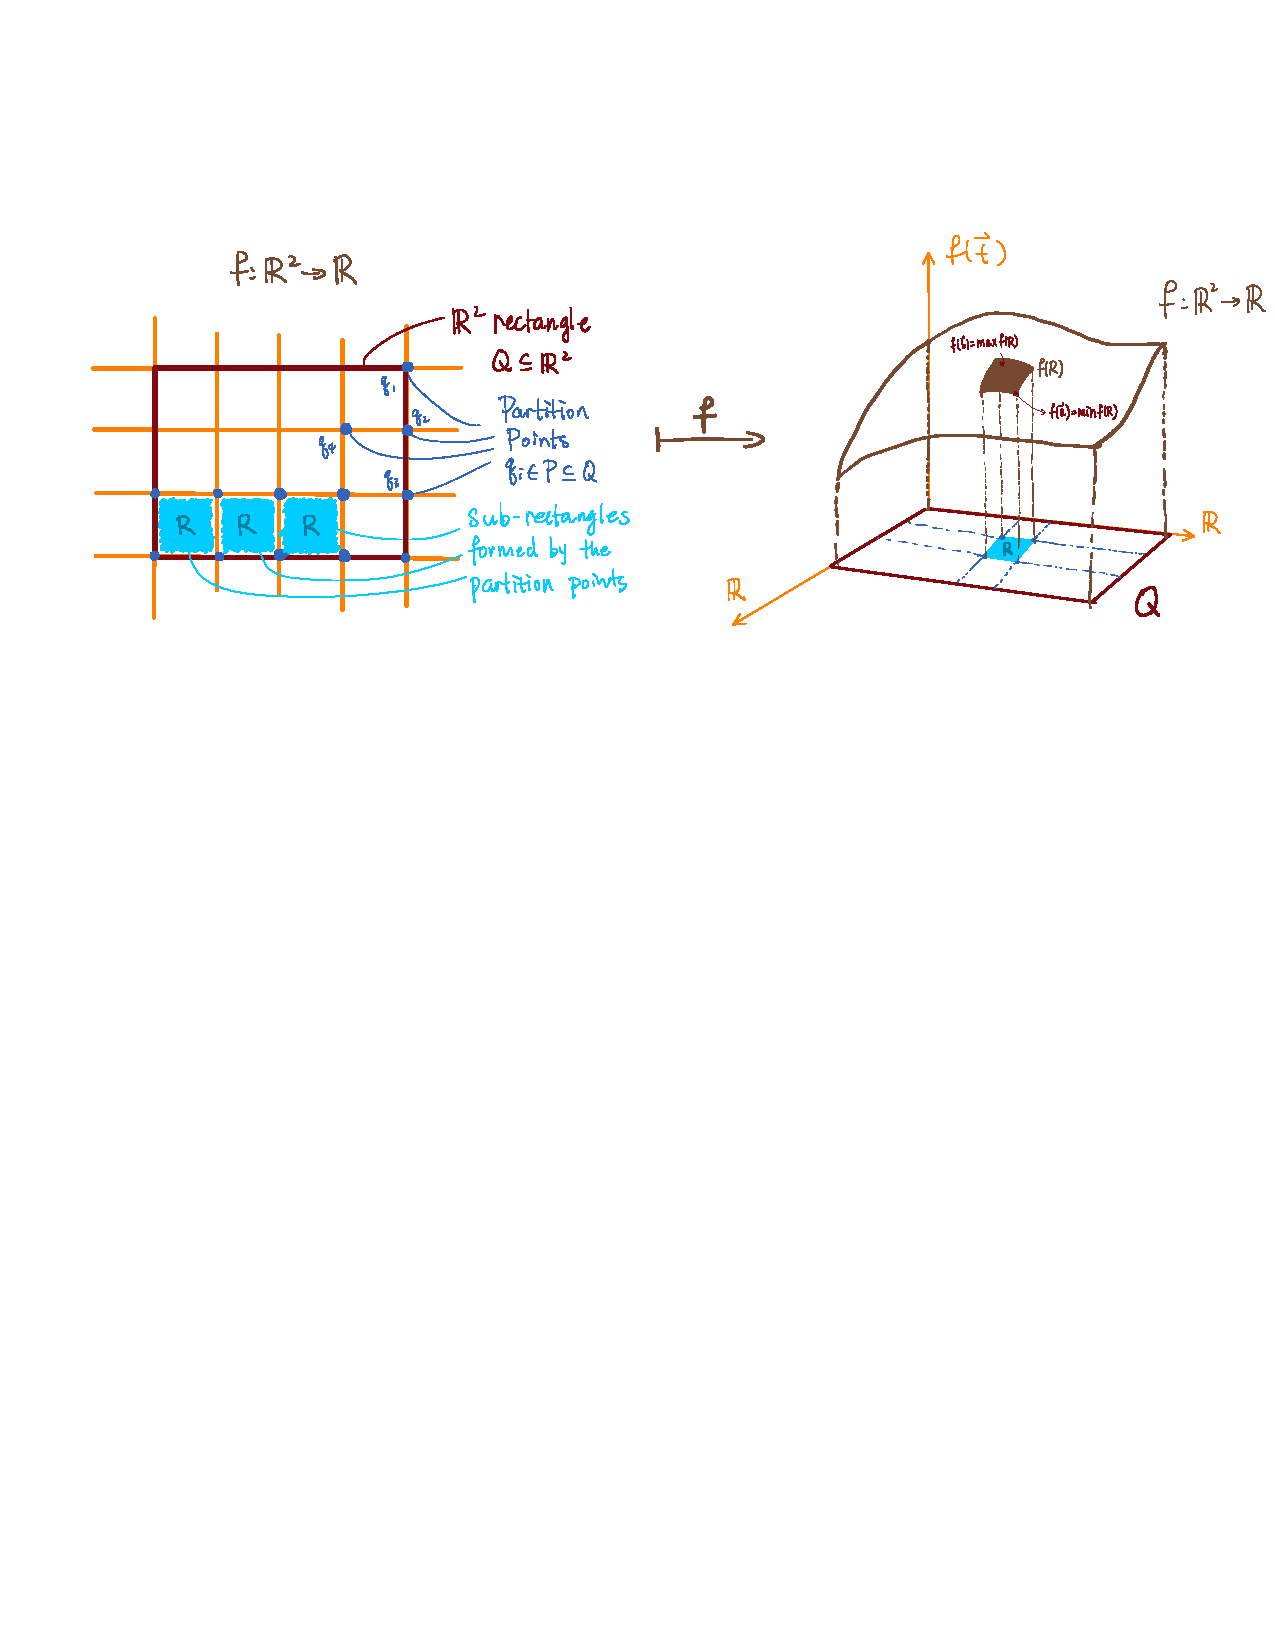
\includegraphics[scale=0.73]{integration.pdf}
\end{center}
We want to fine a way to define the integral $\int_Q$ for bounded functions over $Q$. For $f$ being defined above, bounded function $g:Q \to \R$, and a constant $C \in \R$, $\int_Q$ should satisfies the followings: 

$$\int_Q C = C \cdot V(Q) \qquad\qquad f\leq g \implies \int_Q f \leq \int_Q g \qquad\qquad \int_Q f = \sum_R \int_R f$$

\begin{defn}
For $f:Q \to \R$ with $P$ being a partition of a box $Q\subseteq \R^n$, we define the followings:
$$L(f,P) \coloneqq \sum_R (\inf(f(R))V(R) \qquad\qquad\qquad	U(f,P) \coloneqq \sum_R (\sup(f(R))V(R)$$
\end{defn}

\note From Definition 10.0.0.0.4, it is immediate that $L(f,P) \leq U(f,P)$.

\begin{defn}
Let $P'$ and $P$ be partitions for  a box $Q\subseteq \R^n$, we say $P'$ refines $P$ provided that $P'$ is obtained by adding more partition points to $P$, that is, $P'$ refines $P$ provided that $P \subseteq P'$.  
\end{defn}


\begin{lem}
For bounded function $f:Q \to \R$ with $P$ being a partition of a box $Q\subseteq \R^n$, we have the following:
$$L(f,P) \leq L(f,P') \leq U(f,P') \leq U(f,P)$$
\end{lem}
\begin{proof}
The proof for this Lemma for $n\geq 1$ is on Munkres Lemma 10.1.\\ One might also want to check Spivak pg.255 for $n=1$.
\end{proof}

\begin{lem}
Let $P$ and $P'$ be arbitrary partitions of a box $Q\subseteq \R^n$, and let $f$ be a bounded function from $Q$ to $\R$. Then we have $L(f,P) \leq U(f,P')$. 
\end{lem}
\begin{proof}
First we form a partition $P''$ using all partition points from $P$ and $P'$. Here $P''$ refines $P$ and $P'$. By Lemma 10.0.1, we see that $L(f,P) \leq L(f,P'') \leq U(f,P'') \leq U(f,P')$.
\end{proof}


\begin{defn}
Let $A$ be a subset of $\R$, and let $f:\Power(A) \to \R$ be a bounded function.
$$\inf_{A_i} f(A_i) \coloneqq \inf\{f(A_i) \mid A_i \subseteq A\} \qquad\qquad\qquad \sup_{A_i} f(A_i) \coloneqq \sup\{f(A_i) \mid A_i \subseteq A\}$$
\end{defn}

\begin{defn}
Let $P$ be a partition of a box $Q \subseteq \R^n$, and let $f:Q \to \R$ be a bounded function.\\
The Darboux Upper Integral is defined to be:
$$\upint_Q f \coloneqq \inf_P U(f,P)$$
The Darboux Lower Integral is defined to be:
$$\lowint_Q f \coloneqq \sup_P L(f,P)$$
\end{defn}

\begin{prop}
For a bounded function $f:Q \to \R$ with $Q$ being a box of $\R^n$, we have the following holds: 
$$\lowint_Q f \leq \upint_Q f$$
\end{prop}
\begin{proof}
Combining Lemma 1.0.1 with Lemma 10.0.2, the result follows.
\end{proof}

\begin{defn}
For a bounded function $f:Q \to \R$ with $Q$ being a box of $\R^n$, $f$ is said to be Riemann integrable over $Q$ provided that $\lowint_Q f = \upint_Q f$, in which case we write $\int_Q f \coloneqq \lowint_Q f$.
\end{defn}

\begin{thm}[Cauchy Criterion for Integrability, or the Riemann Condition for Integrability]
For a bounded function $f:Q \to \R$ with $Q$ being a box of $\R^n$, $f$ is Riemann integrable on $Q$ if and only if for all $\epsilon>0$, there exists a partition $P$ such that $U(f,P) < L(f,P) + \epsilon$.
\end{thm}
\begin{proof}
For the $\Leftarrow$ direction, for all $\epsilon>0$, there exists some partition $P$ of $Q$ such that we have:
$$0 \leq \upint_Q f - \lowint_Q f \leq U(f,P) - L(f,P) < \epsilon$$
so we must have $\upint_Q f = \lowint_Q f $ by Lemma 1.0.1, this completes the proof for the $\Leftarrow$ direction. For the $\Rightarrow$ direction, for a given $\epsilon >0$, we see that there exists partitions $P,P'$ of $Q$ with $U(f,P') < L(f,P)+\epsilon$, take refinement $P''$ of $P$ and $P'$, we have $U(f,P'') < L(f,P'')+\epsilon$, the result follows.
\end{proof}


\begin{defn}
Let $Q $ be a box of $\R^n$, the osculation of a bounded function $f:Q \to \R$ at $\vec{a}\in \R^n$ is defined to be: 
$$osc(f,\vec{a}) \coloneqq \inf\left\{ \sup\{ f(\vec{t})\mid \vec{t} \in B_\delta(\vec{a})\cap Q\}  - \inf\{ f(\vec{m})\mid \vec{m} \in B_\delta(\vec{a})\cap Q\}  \mid {\delta>0} \right\} $$
\end{defn}

Let $f:Q \to \R$ be a bounded function with $Q$ being a box of $\R^n$. \\
\note $osc(f,\vec{a}) < \epsilon \iff \exists\ $open neighborhood $U$ of $\vec{a}$ such that $\sup_{U\cap Q} f - \inf_{U\cap Q} f < \epsilon$.\\ 
\note $\{ \vec{a} \in Q,\ osc(f,\vec{a})<\epsilon\}$ is relatively open. $g:Q \to \R \ \ \ \vec{a}\mapsto osc(f,\vec{a})$ is upper semi-continuous.\\

\example
$$f: \R \to \R \ \ \ x\mapsto\begin{cases} \sin(1/x) & x \neq 0 \\ 0 & x = 0\end{cases} \qquad\qquad\qquad osc(f,a) = \begin{cases} 0 & a \neq 0 \\ 2 & a = 0 \end{cases}$$


\begin{defn}
Let $f:Q \to \R$ be a bounded function with $Q$ being a box of $\R^n$. $\D_k(f)\coloneqq \{ \vec{a} \in Q \mid osc(f,\vec{a}) \geq \frac{1}{k}\}$
\end{defn}
 
\note The set $\D_k(f)$ defined in Definition 10.1.0.0.2 is closed.

\begin{defn}
Let $f:Q \to \R$ be a bounded function with $Q$ being a box of $\R^n$. $$\D(f) \coloneqq \bigcup_{k=1}^\infty \D_k(f) = \{\vec{a}\in Q \mid f \text{ is not continuous at } \vec{a}\}$$
\end{defn}
\note The set $\D(f)$ defined in Definition 10.1.0.0.3 is an $F_\sigma$ set.

\begin{defn}
Let $(X,\T)$ be a topological space, let $A$ be a subset of $X$ equipped with the subspace topology inherited from $X$, let $M$ be a subset of $A$, the relative interior of $M$, denoted as $rInt(M)$, is defined to be: $$rInt(M) \coloneqq \{x\in M \mid \exists\ \epsilon >0,\ s.t.\  B_\epsilon(x)\cap A \subseteq M \}$$
\end{defn}

\begin{defn}
Let $A$ be a subset of $R^n$. $A$ is said to have measure zero in 
$R^n$ provided that for every $\epsilon > 0$, there exists countably many boxes $Q_1,Q_2,\cdots$ of $R^n$ such that $A \subseteq \bigcup_{i=1}^\infty Q_i$ with $\sum_{i=1}^\infty V(Q_i)< \epsilon$. 
\end{defn}


\begin{thm}
Let $f:Q \to \R$ be a bounded function with $Q$ being a box of $\R^n$.\\ Given $\epsilon>0$ and some $k \in \N$, the followings are equivalent:
\begin{enumerate}[topsep=3pt,itemsep=-1ex,partopsep=1ex,parsep=1ex]
\item The function $f$ is Riemann integrable on $Q$
\item There exists a partition $P$ such that $U(f,P) < L(f,P) + \epsilon$
\item $\exists$ some subboxes $R_1,R_2,\cdots, R_j$ of $Q$ s.t. $\D_k(f) \subseteq R_1\cup R_2\cup\cdots\cup R_j$ and $\sum_{i=1}^j V(R_i) <\epsilon$ 
\item There exists some subboxes $R_p$ of $Q$ such that $\D(f) \subseteq \bigcup_{p=1}^\infty R_p$, with $\sum_{p=1}^\infty V(R_p) < \epsilon$
\item There exists some subboxes $R_p$ of $Q$ such that $\D(f) \subseteq \bigcup_{p=1}^\infty rInt(R_p)$ with $\sum_{p=1}^\infty V(R_p) < \epsilon$
\end{enumerate}
In the context of this theorem, a box $R$ is called a subbox of $Q$ provided that $R$ is a box in $\R^n$ contained in $Q$, and here $R$ is allowed to have zero volume, or in other words, measure zero.
\end{thm}
\begin{proof}
The equivalency between (1) and (2) is immediate from Theorem 10.1. Now we will show that (2) implies (3). Given $k \in \N$, pick a partition $P$ of $Q$ such that for subboxes $R_i$ determined by $P$, we have the following holds: $$U(f,P) - L(f,P)=\sum_{R_i}\left(\sup_{R_i} f- \inf_{R_i} f\right)V(R) < \epsilon/(19k)$$
Let $R_{i,1},R_{i,2},\cdots, R_{i,l}$ denote the subboxes determined by $P$ that satisfies $Int(R_{i,j}) \cap \D_k(f)\neq \emptyset$, then we can write the following:
$$\frac{1}{k}\sum_{p=1}^l V(R_p) = \sum_{p=1}^l \frac{1}{k} V(R_{i,p}) \leq \sum_{p=1}^l \left(\sup_{R_{i,p}} f - \inf_{R_{i,p}} f\right) V(R_{i,p}) \leq \frac{\epsilon}{19k}\qquad\Rightarrow\qquad \sum_{p=1}^l V(R_{i,p}) < \epsilon$$
Here we note that, $\D_k(f)$ might not necessarily be a subset of $R_{i,1} \cup R_{i,2}\cup\cdots\cup R_{i,l}$ because $\D_k(f)$ might have nonempty intersection with the boundaries of some other subboxes $R_{b,1},R_{b,2},\cdots, R_{b,t}$ determined by $P$, so we can write $\D_k(f)\subseteq R_{i,1}\cup R_{i,2} \cup \cdots R_{i,l} \cup Bd(R_{b,1}) \cup Bd(R_{b,2}) \cup \cdots \cup Bd(R_{b,t})$, where each $Bd(R_{b,j})$ is a finite union of subboxes of $Q$ that have measure zero, hence we have: $$\D_k(f) \subseteq R_{i,1}\cup R_{i,2} \cup \cdots R_{i,l} \cup  R_{z,1}\cup R_{z,2} \cup \cdots \cup R_{z,m}$$
for some zero volume subboxes $R_{z,j}$ of $Q$. With the definition of a box in $\R^n$, it follows that we have $\sum_{p=1}^l V(R_{i,p}) + \sum_{j=1}^m V(R_{z,j}) = \sum_{p=1}^l V(R_{i,p})< \epsilon$. This shows that (2) implies (3). To show that (3) implies (4), for each $k \in \N$, pick finitely many subboxes of $Q$ such that $\D_k(f)$ is contained in the union of the subboxes and the volume sum of those subboxes is less than $\frac{\epsilon}{2^k}$, the result follows. Now we will show (4) implies (5), let $\epsilon>0$ be given, pick subboxes $R_p$ such that $\D(f) \subseteq \bigcup_{p=1}^\infty R_p$ with $\bigcup_{p=1}^\infty V(R_p) < \frac{\epsilon}{19}$. For each $p$, pick suboxes $\hat{R}_p$ of $Q$ such that the following condition holds: \\
(1) If $V(R_p) >0$, then $R_p \subseteq rInt(\hat{R}_p)$ with $V(\hat{R}_p) < 2V(R_p)$\\
(2) If $V(R_p) = 0$, then $R_p \subseteq rInt(\hat{R}_p)$ with $V(\hat{R}_p) < \frac{\epsilon}{2^{p+1}}$ \\
Here we get $\sum_{p=1}^\infty V(\hat{R}_p) < 2\cdot \frac{\epsilon}{19} + \sum \frac{\epsilon}{2^{p+1}} < \epsilon$. This shows that (4) implies (5). Lastly, we will show (5) implies (2). Given $\epsilon>0$, let $\hat{\epsilon} = \frac{\epsilon}{3(M+V(Q))}$ where $M = \max(|f||_Q)$. By assumption, there exists some suboxes $R_p$ such that $\D(f) \subseteq \bigcup_{p=1}^\infty rInt(R_p)$ with $\sum V(R_p)<\hat{\epsilon}$. For each $\vec{a}\in Q \setminus \D(f)$, $f$ is continuous at $\vec{a}$, so there exists a subbox $Q_{\vec{a}}$ of $Q$ with $\vec{a}\in rInt(Q_{\vec{a}})$ and $|f(\vec{x}) - f(\vec{a})| < \hat{\epsilon}$ for $\vec{x}\in Q_{\vec{a}}$. Note here $Q \subseteq \bigcup_{p=1}^\infty rInt(R_p) \cup (\bigcup_{\vec{a}\in Q\setminus \D(f)} rInt(Q_{\vec{a}}))$. Here we note that $Q$ is compact, and each $rInt(Q_{\vec{a}})$, or $rInt(R_p)$, is open, so there exists a finite subcover such that we have:
$$Q \subseteq \left(\bigcup_{p=1}^s rInt(R_{p})\right) \cup \left( \bigcup_{\text{finitely many }\vec{a}\in Q\setminus \D(f)} rInt(Q_{\vec{a}}) \right)$$
Here we denote $rInt(Q_{\vec{a}_1}) \cup rInt(Q_{\vec{a}_2}) \cup rInt(Q_{\vec{a}_t}) = \bigcup_{\text{finitely many }\vec{a}\in Q\setminus \D(f)}$, and $rInt(R_{p_1})\cup rInt(R_{p_2})\cup \cdots, \cup rInt(R_{p_s}) = \bigcup_{p=1}^s rInt(R_{p})$. Pick partition $P'$ such that each subbox $R$ determined by $P'$ satisfies at least one of the two conditions:
(1) $R \subseteq Q_{\vec{a}_j}$, or
(2) $R \subseteq R_{p_k}$.
If $R$ satisfies condition (1), we say $R$ is good, and if $R$ does not satisfies (1), we say $R$ is bad. Then we can write the following:
\begin{align*}
U(f,P) - L(f,P) &= \sum_{R} (\sup_{R} f - \inf_R f) V(R)\\
&= \sum_{good\ R}(\sup_{R} f - \inf_R f) V(R) + \sum_{bad\ R} (\sup_{R} f - \inf_R f) V(R)\\ &\leq \sum_{good\ R} 2\hat{ \epsilon}(R)  + \sum_{bad \ R}2MV(R)\\ &\leq 2\hat{\epsilon}V(Q) + 2M\hat{\epsilon} \\&< \epsilon
\end{align*}
This shows that (5) implies (2). Now we have shown that (2), (3), (4), (5), are equivalent, and we know that (1) and (2) are equivalent by Theorem 10.1, the result of this theorem follows.  
\end{proof}

\begin{lem}
Let $f:Q \to \R$ and $g:Q \to \R$ be function defined on a box $Q \subseteq \R^n$. If we have $f(\vec{x})\leq g(\vec{x})$ for all $\vec{x}$ in $Q$, then we have $\lowint_Q f \leq \lowint_Q g$ and $\upint_Q f \leq \upint_Q g$.
\end{lem}
\begin{proof}
For partition $P$ of the box $Q$, we have $L(f,P) \leq L(g,P) \leq \lowint_Q g$, it follows that $\lowint_Q f \leq \lowint_Q g$. On the  other hand, we have  $\upint_Q f \leq U(f,P) \leq U(g,P)$, it follows that $\upint_Q f \leq \upint_Q g$. A more detailed proof can be found on Section 10 on Munkres. 
\end{proof}

\begin{thm}[Fubini's Theorem]
Let $A$ be a box in $\R^k$, $B$ be a box in $\R^n$, let $Q = A \times B$, and let $f:Q \to \R$ be a bounded function. Then we can write:
$$\lowint_Q f  \leq \lowint_{\vec{x}\in A} \lowint_{\vec{y}\in B}f(\vec{x},\vec{y})\leq \ \ \ \begin{cases}\begin{rcases} \lowint_{\vec{x}\in A} \upint_{\vec{y} B}f(\vec{x},\vec{y}) \\ \upint_{\vec{x}\in A} \lowint_{\vec{y}\in B}f(\vec{x},\vec{y})\ \  \end{rcases}\end{cases}\leq  \upint_{\vec{x}\in A} \upint_{\vec{y}\in B}f(\vec{x},\vec{y})\leq  \upint_Q f$$
\end{thm}
\begin{proof}
By Proposition 10.0.3, we know that $\lowint_Q f \leq \upint_Q f$, we will refer this result as (*). By Lemma 10.2.1, we know that $\lowint_Q f \leq \lowint_Q g$ when $f(\vec{x})\leq g(\vec{x})$ for all $\vec{x}\in Q$, we refer this result as (a). Also by Lemma 10.2.1, we know that $\upint_Q f \leq \upint_Q g$ when $f(\vec{x})\leq g(\vec{x})$ for all $\vec{x}\in Q$, we refer this result as (b). Here we see that, Using result from (*), we get $\lowint_{\vec{x}\in A} \lowint_{\vec{y}\in B} f(\vec{x},\vec{y}) \leq \upint_{\vec{x}\in A} \lowint_{\vec{y}\in B} f(\vec{x},\vec{y})$, and $\lowint_{\vec{x}\in A} \upint_{\vec{y}\in B} f(\vec{x},\vec{y}) \leq \upint_{\vec{x}\in A} \upint_{\vec{y}\in B} f(\vec{x},\vec{y})$. Combining the result from (*) and (a), we get $\lowint_{\vec{x}\in A} \lowint_{\vec{y}\in B} f(\vec{x},\vec{y}) \leq \lowint_{\vec{x}\in A} \upint_{\vec{y}\in B} f(\vec{x},\vec{y})$. Combining the result from (*) and (b), we get $\upint_{\vec{x}\in A} \lowint_{\vec{y}\in B} f(\vec{x},\vec{y}) \leq \upint_{\vec{x}\in A} \upint_{\vec{y}\in B} f(\vec{x},\vec{y})$. To show $\lowint_Q f \leq \lowint_{\vec{x}\in A} \lowint_{\vec{y}\in B}f\left(\vec{x},\vec{y}\right)$, we denote $\vec{x}_0 \in R_A$ where $R_A$ is a subrectangle of $A$, denote $R_b$ as subrectangle of $B$, we can write: $$\lowint_{\vec{y}\in B} f\left(\vec{x}_0, \vec{y}\right) \geq \sum_{R_B} \inf_{\vec{y}\in R_B} \left(f\left(\vec{x}_0,\vec{y}\right)\right) \cdot V\left(R_B\right) \geq \sum_{R_B} \inf_{R_A \times R_B}\left(f\right)\cdot V\left(R_B\right) $$
On the other hand, we have:
\begin{align*}
\lowint_{\vec{x}\in A }\left(\lowint_{\vec{y}\in B} f\left(\vec{x},\vec{y}\right)\right) &\geq  \sum_{R_A} \inf_{\vec{x}\in R_A} \left(\lowint_{\vec{y}\in B}f\left(\vec{x},\vec{y}\right)\right) V\left(R_A\right)\\
&\geq \sum_{R_A}\sum_{R_B} \inf_{R_A\times R_B} \left(f\right) V\left(R_A \times R_B\right) \\
&= L\left(f,P\right)
\end{align*}
Hence we see that $\lowint_Q f \leq \lowint_{\vec{x}\in A} \lowint_{\vec{y}\in B} f(\vec{x},\vec{y})$. Lastly, one can show that $\upint_{\vec{x}\in A} \upint_{\vec{y}\in B} f(\vec{x},\vec{y}) \leq \upint_Q f$ by combining $\lowint_Q f \leq \lowint_{\vec{x}\in A} \lowint_{\vec{y}\in B} f(\vec{x},\vec{y})$ with the fact that $\upint_Q f = -\lowint_Q  (-f)$.  This completes the proof of this theorem.
\end{proof}


\newpage
\begin{corT}
Let $A$ be a box in $\R^k$, $B$ be a box in $\R^n$, let $Q = A \times B$, and let $f:Q \to \R$ be a bounded function. If $f$ is integrable on $Q$, then we have:
$$\lowint_Q f  = \lowint_{\vec{x}\in A} \lowint_{\vec{y}\in B}f(\vec{x},\vec{y})= \ \ \ \begin{cases}\begin{rcases} \lowint_{\vec{x}\in A} \upint_{\vec{y} B}f(\vec{x},\vec{y}) \\ \upint_{\vec{x}\in A} \lowint_{\vec{y}\in B}f(\vec{x},\vec{y})\ \  \end{rcases}\end{cases}= \upint_{\vec{x}\in A} \upint_{\vec{y}\in B}f(\vec{x},\vec{y})=  \upint_Q f$$ 
and we can write:
$$\int_Q f = \int_{\vec{x}\in A}\upint_{\vec{y}\in B}f(\vec{x},\vec{y}) = \int_{\vec{x}\in A}\lowint_{\vec{y}\in B} f(\vec{x},\vec{y})$$
\end{corT}
\note Given the settings in Corollary 10.3.1, $\int_{\vec{y}\in B} f(\vec{x},\vec{y})$ may not necessarily exist. 



\begin{corT}
A function $f$ is continuous on $Q = I_1 \times \cdots \times I_n$ implies $\int_Q f = \int_{x_1\in I_1}  \int_{x_{n-1} \in I_{n-1}} \int_{x_n \in I_n} f(x_1,\cdots, x_n)$
\end{corT}


\begin{lem}
Let $R$ be a subbox of a box $Q\in \R^n$. \\
For $y > V(R)$, there exists a subbox $\hat{R}$ of $Q$ with $R \subseteq rInt(\hat{R}) \subseteq Q$ such that $V(\hat{R})<y$. 
\end{lem}

\note Consider a bounded function defined on a box $Q$.
\begin{enumerate}[topsep=3pt,itemsep=-1ex,partopsep=1ex,parsep=1ex]
\item If $f^{-1}(0)$ is dense in $Q$, then all $L(f,P) \leq 0$, all $U(f,P) \geq 0$, which implies $\lowint_Q f \leq 0 \leq \upint_Q f$.
\item If $f^{-1}(0)$ is dense in $Q$ and $f$ is integrable, then $\int_Q f = 0$.
\item If $f \geq 0$, $f(\vec{a}) > 0$, $f $ is continuous at $\vec{a}$, then $\lowint_Q f > 0$. 
\item If $f \geq 0$, $f(\vec{a}) > 0$, and $\lowint_Q f =0$, then $f$ is discontinuous.
\item If $f \geq 0$ and $f$ is integrable on $Q$, with $\int_Q f = 0$, then $Q \setminus f^{-1}(0)$ has measure zero. 
\end{enumerate}
\begin{proof}[Proof of (3)]
Choose partition $P$ such that $f > \frac{f(\vec{a})}{2}$ on some boxes $R^*$ determined by $P$. Then we can write $\lowint_Q f \geq L(f,P) = \inf_{R^*} (f)\cdot V(R^*) + \sum_{R} \inf_R f\cdot V(R) \geq \frac{f(\vec{a})}{2}V(R^*)+ 0 $.
\end{proof}

\example Let $Q = [-1,1] \times [-1,1]$, and $f = \mathbb{I}_{\{0\} \times \Q}$, where $\mathbb{I}$ is the indicator function, we see that $\D(f) = \{0\} \times [-1,1]$, which is a set that has zero measure, so we know that $f$ is integrable on $Q$. Notice that, integrating over $y$ with fixed $x$, we have the followings:
$$\upint_{y \in [-1,1]} f(x,y)  = \begin{cases} 
0& x\neq 0 \\ 1 & x = 0
\end{cases} \qquad \qquad \qquad \lowint_{y \in [-1,1]} f(x,y) = \begin{cases} 0 & x \neq 0 \\ 0 & x= 0 \end{cases}$$
One might also integrate over $x$ with fixed $y$ and get $\int_{x \in [-1,1]} f(x,y) = 0$. From Fubini's Theorem, we can write $\int_Q f = 0$. \\




\newpage
\section[Integrating Over a Bounded Set]{\color{red} Integrating Over a Bounded Set \color{black}}


\begin{defn}
Let $S$ be a bounded subset of $\R^n$, and let $f:S \to \R$ be a bounded function.
$$f_S : \R^n \to \R \qquad \vec{x}\mapsto \begin{cases}f(\vec{x}) & \vec{x} \in S \\ 0 &\vec{x}\notin S\end{cases} \qquad \qquad \qquad\int_S f \coloneqq \int_Q f_S \quad \text{for box } Q \text{ that contains }S$$
\end{defn}

\begin{prop}
Let $S$ be a bounded subset of $\R^n$, and let $f:S \to \R$ be a bounded function. \\The existence and the value of $\int_Q f_S$ does not depend on the choice of the box $Q$ which contains $S$.
\end{prop}


\begin{proof}
For the existence of $\int_Q f_S$, let $Q_1,Q_2$ be boxes that contain $S$, and let $Q_3$ be a box of $S$ such that $Q_1$ and $Q_2$ are contained in the interior of $Q_3$. 

\begin{center}
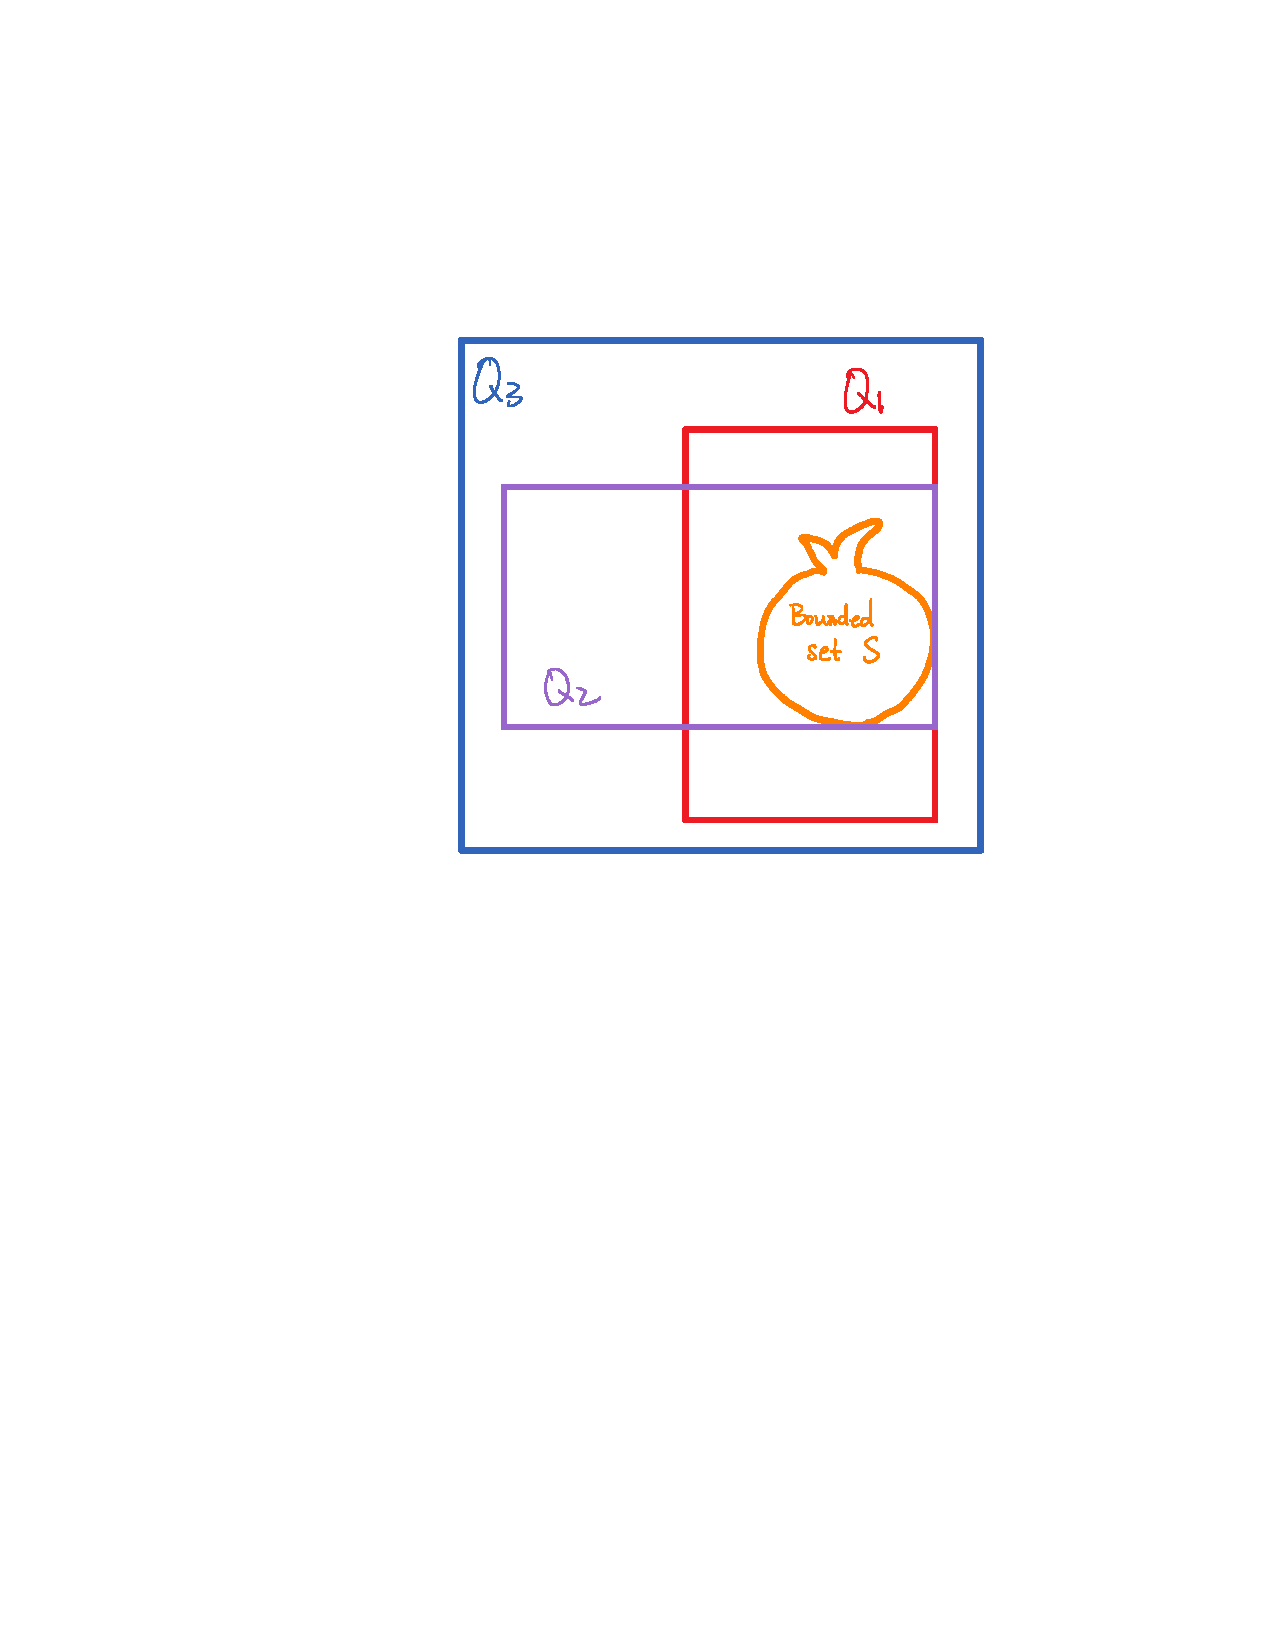
\includegraphics[scale=0.5]{IntOverBddSet.pdf}
\end{center}

We will investigate $\D(f_S)$ on $Q_3$, denoted as $\D(f_S)_3$, and $\D(f_S)$ on $Q_1$, denoted as $\D(f_S)_1$. We see that $\D(f_S)_3 = \D(f_S)_1 \cup \{ \text{subset of }Bd(Q_1)\}$, here $\{ \text{subset of }Bd(Q_1)\}$ can be covered by finitely many zero-volume boxes. Here we conclude that $f_S$ is integrable on $Q_1$ if and only if $f_S$ is integrable on $Q_3$ by Theorem 10.2, and similarly, $f_S$ is integrable on $Q_2$ if and only if $f_S$ is integrable on $Q_3$. Now we can conclude that $f_S$ is integrable on $Q_1$ if and only if $f_S$ is integrable on $Q_2$. That is, the integrability of $f_S$ does not depend on the choice of $Q$. Now we will show that $\int_{Q_1} f_S = \int_{Q_3} f_S$. Let $P $ be a partition of $Q_3$, and refine $P$ to $P'$ such that $Q_1$ is contained in a finite union of boxes determined by $P'$. We denote the boxes determined by $P'$ as $P'-$boxes. Then we can write:
\begin{align*}
L(f_S,P) \leq L(f_S, P') &= \sum_{\substack{P' \text{-boxes } R  \\ \text{ contained in } Q_1}} \inf_R (f_S) V(R) \quad + \sum_{\substack{\text{other }P'\text{-boxes } R' \\ \text{ contained in }Q \setminus rIntQ_1}} \inf_{R' }(f_S) V(R') \leq \lowint_{Q_1} f_S
\end{align*}
Here we can take the supremum over choice of $P$ to get $\int_{Q_3} f_S \leq \int_{Q_1} f_S$. With similar argument, we get $\int_{Q_3} f_S \geq \int_{Q_1} f_S$ using $U(f_S,P)$, and the result follows. 
\end{proof}

\note The proof of the followings can be found on Section 13 in Munkres, and Chapter 13 in Spivak. \\
Let $S\subseteq \R^n$ be bounded, let $a,b \in \R$, and let $f:Q \to \R$ and $g:Q \to \R$ be integrable functions.
\begin{enumerate}[topsep=3pt,itemsep=-1ex,partopsep=1ex,parsep=1ex]
\item $\int_S(af+bg) = a\int_S f + b\int_S g$
\item If $f(\vec{x})\leq g(\vec{x})$ for all $\vec{x}\in S$, then we have $\int_S f \leq \int_S g$
\item $|f|$ is integrable on $S$
\item If $f_S$ is continuous, then $|f|_S$ is continuous. 
\item $|\int_S f| = \max\{ (\int_S f),\ (- \int_S f)\} \leq \int_S |f|$
\item Let $T \subseteq S$, if $f(\vec{x}) \geq 0$ for all $\vec{x}\in S$,  and $f$ is integrable on $T$, then $\int_T f \leq \int_S f$. 
\item If $f$ is integrable on bounded sets $S_1$ and $S_2$, then $f$ is integrable on $S_1 \cup S_2$ and $S_1 \cap S_2$, with $$\int_{S_1\cup S_2} = \int_{S_1} f + \int_{S_2} f - \int_{S_1\cap S_2} f$$
\end{enumerate}
\begin{proof}[Proof of (7)]
Let $A = \{ (x,y) \in \R^2 \mid x=0 \text{ or }y=0 \text{ or }x=y\}$. Let $\phi:A \to \R$ be defined by:
$$\phi:A \to \Q \qquad \begin{cases}(x,0) \mapsto x \\ (0,y) \mapsto y \\ (x,x) \mapsto x    \end{cases}$$
It is easy to check that $\phi$ is continuous, and we have $\phi(f_{S_1}, f_{S_2}) = f_{S_1\cup S_2}$, so we know that $f_{S_1\cup S_2} $ is continuous at the points where $f_{S_1}$ and $f_{S_2}$ are continuous. The discontinuous sets for $f_{S_1}$ and $f_{S_2}$ satisfies the condition of Theorem 10.2 because $f$ is integrable on $S_1$ and $S_2$, then it follows that the discontinuous set for $f_{S_1\cup S_2}$ also satisfies the condition in Theorem 10.2, and hence $f_{S_1\cup S_2}$ is integrable on $S_1 \cup S_2$, where one can easily show that $f_{S_1\cup S_2}+ f_{S_1\cap S_2} = f_{S_1} + f_{S_2}$. 
\end{proof}


\exercise Let $S = \{(x_1,x_2,x_3) \mid x_1 \geq 0,\ x_2\geq 0,\ x_3 \geq 0,\ x_1+x_2+x_3 \leq 1 \}$, here $S$ is a tetrahedron, or a $3$-simplex, with $S = ch( \vec{e}_1,\vec{e}_2,\vec{e}_3,\vec{0})$. Let $Q = [0,1]\times[0,1]\times[0,1]\supset S$, we have: 
\begin{align*}
\int_S 1 = \int_{Q} \mathbb{I}_S 
&= \int_{0\leq x_1\leq 1} \int_{0\leq x_2 \leq 1} \int_{0\leq x_3 \leq 1} \mathbb{I}_S 
\\&= \int_{0\leq x_1 \leq 1} \int_{0\leq x_2 \leq 1} \max\{ 1-x_1-x_2, 0\} 
\\&= \int_{0 \leq x_1 \leq 1} \int_{0 \leq x_2 \leq 1-x_1} 1-x_1-x_2
\\&= \int_{0\leq x_1 \leq 1} \left[(1-x_1) x_2 - \frac{x_2^2}{2}\right]^{x_2 = 1-x_1}_{x_2 = 0}
\\&= \int_{0\leq x_1 \leq 1} \frac{(1-x_1)^2}{2} = \left[-\frac{(1-x_1)^3}{2}\right]_{x_1 = 0}^{x_1=1} = \frac{1}{6}
\end{align*}





\begin{defn}
Let $E$ be a subset of $\R^n$. $$m^*(E) \coloneqq  \inf\left\{\sum_{j=1}^\infty V(Q_j) \mid E \subseteq \bigcup_{j=1}^\infty Q_j, \text{ where } Q_j \text{ are boxes in }\R^n \right\} $$
Here $m^*(E)$ is called the outer Lebesgue measure of $E$.
\end{defn}

\note A set $E$ has outer Lebesgue measure $0$ provided that $m^*(E) = 0$, if and only if $E$ has measure $0$ as described in Munkres Section 11 and Math 395 IBL. \\
\remark Here we do not allow arbitrary coverage by boxes to avoid having $m^*(E) \equiv 0$.\\
\remark Here we allow infinite coverings. We might consider building the theory using finite coverings, called the outer Jardon measure, defined by the following when $E\subseteq \R^n$ is bounded:
$$m^{*,J}(E) \coloneqq  \inf\left\{\sum_{j=1}^k V(Q_j) \mid E \subseteq \bigcup_{j=1}^k Q_j, \text{ where } Q_j \text{ are boxes in }\R^n \right\} $$
and setting $m^{*,J}(E) \coloneqq \infty$ when $E$ is unbounded. 


\note For a set $E\subseteq \R^n$, we have $m^*(E) \leq m^{*,J}(E)$.
\begin{prop}
For sets $E_j\subseteq \R^n$.\\ If $m^*(E_j) = 0$ for $j=1,2,\cdots$, then we have $m^*(\bigcup_{j=1}^\infty E_j) = 0$. \\If $m^{*,J}(E_j) = 0$ for $j=1,2,\cdots$, then we have $m^{*,J}(\bigcup_{j=1}^\infty E_j) = 0$.
\end{prop}
\begin{proof}
The proof of this proposition is given on Munkres Theorem 11.1.
\end{proof}


\begin{lem}
For $E \subseteq \R^n$, we have: 
$$m^*(E) = \inf\left\{\sum_{j=1}^\infty V(Q_j) \mid E \subseteq \bigcup_{j=1}^\infty \text{Int}(Q_j) , \text{ where } Q_j \text{ are boxes in }\R^n \right\}$$
$$m^{*,J}(E) = \inf\left\{\sum_{j=1}^k V(Q_j) \mid E \subseteq \bigcup_{j=1}^k \text{Int}(Q_j ), \text{ where } Q_j \text{ are boxes in }\R^n\right\} $$
here we use relative interior when appropriate. 
\end{lem}
\begin{proof}
Comparing to the definition of the Lebesgue and Jardon measure, such restrictions in this Lemma can only increase the infimum. Hence we need to show no increase in the infimum occurs. For the case $m^*(E) = \infty$, the result follows trivially. Let $\epsilon>0$ be given, for nonempty $E$, pick $\widetilde{Q}_j \supseteq Int(\widetilde{Q}_j) \supseteq Q_j$ with $V(\widetilde{Q}_j) < V(Q_j) + \frac{\epsilon}{2^j}$, by Lemma 10.3.3, here we get $Int(\widetilde{Q}_j)$ covering $E$ with $\sum V(\widetilde{Q}_j) < \sum V(Q_j) + \epsilon$. Since $\epsilon$ is arbitrary, we see that there is no change in infimum. 
\end{proof}
\newpage

\begin{prop}
Let $K$ be a compact subset of $\R^n$, then we have $m^{*,J}(K) = m^*(K)$
\end{prop}
\begin{proof}
It suffices to show that $m^*(K) \geq m^{*,J}(K)$ holds. Pick $Q_j$ with $\bigcup_{j=1}^\infty Int(Q_j) \supseteq K$. By compactness of $K$, there exists $M \in \N$ such that $\bigcup_{j=1}^M Int(Q_j) \supseteq K$, then we can write:
$$\sum_{j=1}^\infty V(Q_j) \geq \sum_{j=1}^M V(Q_j) \geq m^{*,J}(K)$$
Now take infimum over choice of $Q_j$'s to get the desired result.
\end{proof}


\note In general, $m^{*,J}(E) \neq m^{*} (E)$ for $E \subseteq \R^n$.\\
\example Let $E = Q \cap [0,1]$, we have $m^*(E) = 0 \neq m^{*,J}(E) = 1$. 



\begin{defn}
Let $S$ be a bounded subset of $\R^n$, let $f:S \to \R$ be a bounded function. $$f_S: \R^n \to \R \ \ \ \vec{x}\mapsto\begin{cases} f(\vec{x}) & \vec{x}\in S \\ 0 & \vec{x}\notin S\end{cases}$$ 
The function $f$ is said to be Riemann integrable on $S$ provided that the function $f_S$ is Riemann integrable on a box $Q$ that contains $S$. 
\end{defn}


\begin{thm}
Let $S$ be a bounded subset of $\R^n$, let $f:S \to \R$ be a bounded continuous function, let $E = \{ \vec{x}_0 \in Bd(S) \mid\lim_{\vec{x}\in S,\ \vec{x}\to \vec{x}_0} f(\vec{x}) \neq 0 \}$. If we have $m^*(E) = 0$, then $f$ is Riemann integrable on $S$. 
\end{thm}
\begin{proof}
Note that $E$ also contains isolated points of $S$, and for such isolated point $\vec{p}$, if exists, $\exists\ \epsilon >0$ such that $\#(B_\epsilon(\vec{p}) \cap S) = 1$, and $\vec{p}\notin \D(f_S)$. Here we have $\D(f_S) \subseteq E$, the result follows immediately from Theorem 10.2. 
\end{proof}

\begin{corT}
Let $S$ be a bounded subset of $\R^n$, let $f:S \to \R$ be a bounded continuous function.\\ 
If $m^*(Bd(S)) = 0$, then $f$ is Riemann integrable on $S$. 
\end{corT}

\begin{defn}
A bounded set $S \subseteq \R^n$ is said to be rectifiable provided that any one of the following holds:
\begin{enumerate}[topsep=3pt,itemsep=-1ex,partopsep=1ex,parsep=1ex]
\item The function $\mathbb{I}:S \to \R \ \ \ \vec{x}\mapsto 1$ is Riemann integrable on $S$
\item The indicator function $\mathbb{I}_S$ is integrable on some box $Q\subseteq \R^n$ that contains $S$.
\item $m^*(Bd(S)) = 0$
\item $m^{*,J}(Bd(S)) = 0$
\end{enumerate} 
\end{defn}
\note By Corollary 10.4.1, if a bounded set $S\subseteq \R^n$ is rectifiable, then all bounded continuous functions defined on the set $S$ are integrable.

\begin{defn}
Let $S\subseteq \R^n$ be a rectifiable set, let $\mathcal{I}:S \to \R \ \ \ \vec{x}\mapsto 1$. $V(S) \coloneqq \int_{S} \mathcal{I}$.
\end{defn}


\note Let $S\subseteq \R^n$ be a rectifiable set, let $A = Int(S)$. Then we have $Bd(A) \subseteq Bd(S) \ \Rightarrow  m^*(Bd(A)) \leq m^*(Bd(S)) = 0\ \Rightarrow A$ is rectifiable $\Rightarrow \mathbb{I}_S$ and $\mathbb{I}_A$ are integrable, where $\mathbb{I}_S,\,\mathbb{A}$ are indicator functions on $S$ and on $A$. Moreover, $\mathbb{I}_{S\setminus A}= \mathbb{I}_S - \mathbb{I}_A$ is integrable on a box $Q$ that contains $\bar{S}$ $\Rightarrow S\setminus A$ is rectifiable, $Int(S\setminus A) = \emptyset$, for all partition $P$, $L(\mathbb{I}_{S\setminus A}, P) = 0 \ \Rightarrow\ \int_Q \mathbb{I}_{S\setminus A} = 0\ \Rightarrow \ \int \mathbb{I}_A = \int \mathbb{I}_S\  \Rightarrow \ V(A) = V(S)$ \\


\newpage
\section[Extended Riemann Integral]{\color{red}Extended Riemann Integrals \color{black}}

In this section we will discuss the integrability of a function $f$ defined on a set $S\subseteq \R^n$, not necessarily bounded, with the property that $f$ is not necessarily bounded. We will focus on discussing the integrability of a continuous real-valued function $f$ defined on an open set $A\subseteq \R^n$, with $A$ and $f$ being not necessarily bounded. \textbf{We will start by assuming that $f(\vec{a}) \geq 0$ for all $\vec{a}\in A$.}

\begin{defn}
Let $A$ be an open subset of $\R^n$, and let $f:A \to \R$ be a continuous function with $f(\vec{a}) \geq 0,\ \forall\vec{a}\in A$. 
$$ext \int_A f \coloneqq \sup\left\{ \int_E f  \mid E \text{ is a compact rectifiable set that is contained in } A\right\}$$
Here $ext \int_A f$ is called the Extended Riemann Integral of $f$ on $A$.
\end{defn}

\begin{lem}
Let $A$ be an open subset of $\R^n$ and let $B$ be an open subset of $A$, then $ext \int_B f  \leq ext \int_A f$ for non-negative function $f$ defined on $A$ and on $B$. 
\end{lem}

\begin{defn}
For bounded open set $A\subseteq \R^n$ and bounded non-negative continuous function $f$ defined on $\R^n$. $$\lowint_A f \coloneqq \lowint_Q f_A$$ for a box $Q$ that contains $A$.
\end{defn}

\note For bounded open $A\subseteq \R^n$ and bounded non-negative continuous function $f$ defined on $\R^n$.
\begin{enumerate}[topsep=3pt,itemsep=-1ex,partopsep=1ex,parsep=1ex]
\item When $A$ is rectifiable, then $\int_A f$ exists.
\item For compact rectifiable subset $E$ of $A$, we have $\int_E f = \lowint_E f \leq \lowint_A f$, so $ext \int_A f \leq \lowint_A f$.
\item Let $P$ be a partition of a box $Q$ that contains $A$, let $M$ be the union of all the boxes determined by $P$ that are contained in $A$, we have $L(f_A, P ) \leq \int_{M} f \leq ext \int_A f$, so $\lowint_A f \leq ext \int_A f$.
\item Combining (2) and (3) we have $\lowint_A f = ext \int_A f$.
\item From (4), we conclude that if $f$ is integrable on $A$, then $\int_A f = ext\int_A f$
\end{enumerate}

\begin{lem}[Computational Methods for Extended Riemann Integral]
Let $E_1\subseteq E_2\subseteq E_3\subseteq \cdots \subseteq A\subseteq \R^n$ with each $E_j$ being compact rectifiable, $\bigcup_j Int(E_j) = A$, and $A$ being open. We have $ext \int_A f = \lim_{j \to \infty} \int_{E_j} f$ for non-negative continuous function $f:\R^n \to \R$. 
\end{lem}
\begin{proof}
We have each of $\int_{E_j} f \leq ext\int_A f$. So $\lim_{j\to \infty} \int_{E_j} f \leq ext \int_A f$. If $E\subseteq A$ is compact rectifiable, then by the compactness of $E$, we have $E\subseteq E_M$ for some $M$, because $E\subseteq Int (E_1) \cup Int(E_2) \cup \cdots \cup Int(E_M) = Int (E_M) \subseteq E_M$. Here we can write $\int_E f \leq \int_{E_M} f \leq \lim_{j \to \infty} \int_{E_j} f$, so we have $ext \int_A f \leq \lim_{j \to \infty} \int_{E_j} f$. The result follows.
\end{proof}
\note Given the setting in Lemma 12.0.2. It is not automatic to have $\bigcup E_j = A$. As an example, consider $E_j = [-j,0] \cup [\frac{1}{j},j]$, we have $\bigcup E_j = \R$, and $\bigcup Int(E_j) = \R\setminus \{0\}$. 

\begin{prop}
For open subset $A$ of $\R^n$. One can always find $E_j$ that satisfies $E_1\subseteq E_2\subseteq E_3\subseteq \cdots \subseteq A$ with each $E_j$ being compact rectifiable, and $\bigcup_j Int(E_j) = A$.
\end{prop}
\begin{proof}
One might propose a proof that is similar to the proof of Lemma 15.1 on Munkres. Alternatively, one can construct each $E_j$ by letting $E_j$ be the union of all closed hyper cubes, where each cube has side length $\frac{1}{2^{j}}$, each cube is a subset of $A$, and the vertex of each cube has coordinates in $\frac{\Z}{2^j} \cap [-j, j]$.
\end{proof}

\hfill\break
\example $$\int_\R \frac{1}{1+x^2} = \lim_{j \to \infty} \int_{\{x \mid -j \leq x \leq j\}}\frac{1}{1+x^2} = \lim_{j\to \infty} \arctan(x)]_{x=-j}^{x=j} = \lim_{j \to \infty} 2\arctan(j) = \pi$$

\newpage

\example 
\begin{align*}
\int_{\R^2} \frac{1}{1+x^2+y^2} &= \lim_{j\to \infty} \int_{\{x \mid -j \leq x\leq j\}\times \{y \mid  -j\leq y \leq j\}} \frac{1}{1+x^2+y^2} \\
&= \lim_{j\to \infty} \int_{\{y \mid -j\leq y \leq j\}} \int_{\{x \mid -j \leq x\leq j\}} \frac{1}{1+x^2+y^2} 
\\&= \lim_{j\to \infty} \int_{\{ y \mid -j \leq y \leq j\}} \frac{2\arctan\left((1+y^2)^{-\frac{1}{2}}\right)}{\sqrt{1+y^2}}
\end{align*}
To evaluate such integral, one might want to use the Risch Algorithm to determine whether such integral is an elementary function. However, there is another easier approach, by Spivak Chapter 24 Theorem 1, we can rewrite the following: 
\begin{align*}
\int_{\R^2} \frac{1}{1+x^2+y^2} &= \lim_{j \to \infty} \lim_{k \to \infty} \int_{\{x \mid -k\leq x \leq k \}\times\{y \mid -j \leq y \leq j\}} \frac{1}{1+x^2+y^2} \\&= \lim_{j \to \infty} \int_{-j}^j \left(\lim_{k \to \infty} \int_{-k}^k \frac{1}{1+x^2+y^2} \, dx\right)\, dy 
\\&= \lim_{j \to \infty} \lim_{k \to \infty} \int_{-j}^j \frac{2\arctan \left(k(1+y^2)^{-\frac{1}{2}}\right)}{\sqrt{1+y^2}} dy 
\\&= \lim_{j \to \infty} \int_{-j}^{j} \frac{\pi}{\sqrt{1+y^2}}\, dy
\end{align*}
Let $y = \sinh (u)$, we get: $\lim_{j \to \infty} \int_{-j}^{j} \frac{\pi}{\sqrt{1+y^2}}\, dy = \lim_{j\to \infty} \pi u ]_{u=-arcsinh (j)}^{u = arcsinh (j)} = \pi(\infty) - \pi(-\infty) = \infty$. \\

\note We conclude the results from above: Let $A $ be an open subset of $\R^n$, let $f \in C(A, [0,\infty))$. $ext \int_A  = \int_A f$ if $\int_A f$ exists. $ext \int_A f = \lim_{j\to \infty} \int_{E_j} f$ provided that each $E_j$ is a compact rectifiable subset of $A$, $E_1 \subseteq E_2 \subseteq \cdots \subseteq A$, and $\bigcup_{j} Int(E_j) = A$. 

\begin{lem}
Let $f:\R^n \to \R$ be non-negative continuous function, let $A$ be open subset of $\R^n$, let $U_1,U_2,\cdots$ be open subsets of $A$ with $U_1 \subseteq U_2 \subseteq \cdots \subseteq A$, and $\bigcup_{j}{U_j} = A$. We have $ext\int_A f = \lim_{j\to \infty} ext\int_{U_j} f$.
\end{lem}
\begin{proof}
Note here $ext\int_A f$ exists as the sequence $(ext\int_{U_j} f)$ is monotonic. Now we write each $ext\int_{U_j} f \leq ext \int_A f$, hence we have $\lim_{j\to \infty} ext\int_{U_j} f \leq ext \int_A f$. For each compact rectifiable $E$ subset of $A$, one can find finite subcover $U_j$ such that $E \subseteq U_1 \cup \cdots \cup U_j$, so we can write $\int_E f \leq ext\int_{U_j} f \leq \lim_{j\to \infty} ext \int_{U_j} f$. Take supremum over the choice of $E$, then we have $ext \int_A f \leq  \lim_{j\to \infty} ext\int_{U_j} f$. This completes the proof. 
\end{proof}

\begin{defn}
For $x \in [-\infty, \infty]$: $$x_+ \coloneqq \max\{x,0\}\qquad\qquad\qquad x_- \coloneqq \max\{-x,0\}$$
\end{defn}
\note For $x\in[-\infty, \infty] $, both $x_+$ and $x_-$ are non-negative. $x_+ \cdot x_- = 0$, $x = x_+ - x_-$, $|x| = x_++x_-$. 
\remark Alternatively, for $x\in[-\infty, \infty] $, one might define $x_+ = \frac{|x|+x}{2}$ and $x_- = \frac{|x|-x}{2}$ instead.\\

In the discussion below, we will consider continuous function $f:\R^n \to \R$, not necessarily non-negative.

\begin{defn}
Let $X$ be a set, for $f:X \to [-\infty, \infty]$:
$$f_+: x\mapsto(f(x))_+ \qquad\qquad\qquad f_-: x\mapsto (f(x))_-$$ 
\end{defn}

\begin{defn}
Let $X$ be a set, let $f:X \to \R$ be a function. \\
If $f$ is non-negative, we denote $f\geq 0$. If $f$ is non-positive, we denote $f\leq 0$.\\
If $f$ is negative, we denote $f< 0$. If $f$ is positive, we denote $f> 0$.
\end{defn}



\note For $f:X \to [-\infty, \infty]$,  $f_+ \geq 0$, $f_- \geq 0$, $f_+\cdot f_- = 0$, $f = f_+ - f_-$, and $|f| = f_+ + f_-$.



\begin{defn}
For $f \in C(A,\R)$ where $A$ is an open subset of $\R^n$. $f$ is said to be extended-integrable on $A$, or integrable on $A$ in the extended sense, provided that both $ext \int_A f_+< \infty$ and $ext \int_A f_- < \infty$ holds. In other words, $f$ is extended-integrable on $A$ provided that $ext \int_A f_+ + ext \int_A f_- = ext \int_A |f| < \infty$. If $f$ is extended-integrable on $A$, then\footnote{By Munkres, $ext \int_A f$ exists provided that $f$ is extended-integrable on $A$. For the purpose of this course, Professor Barrett propose another definition for the existence of $ext \int_A f$, given in Definition 12.0.4.0.5} we write $ext \int_A f \coloneqq ext \int_A f_+ - ext \int_A f_-$. 
\end{defn}

\begin{defn}
For $f \in C(A,\R)$ where $A$ is an open subset of $\R^n$, \\$ext \int_A f$ exists \footnote[1]{In the rest of this text, the existence of $ext \int_A f$ refers to Definition 12.0.4.0.5} provided that at least one of $ext \int_A f_+$ and $ext \int_A f_-$ is finite.
\end{defn}


\exercise Let $f$ be a real-valued continuous bounded non-positive function defined on an open subset $A $ of $\R^n$. Then we have $f_- = -f$, and here $ext \int_A f = -ext\int_A (-f) = -\lowint_A (-f) = \upint_A f$. \\

\begin{lem}
Let $a,b\in \R$, let $f:A \to \R$ and $g:A \to \R$ be continuous functions that are extended-integrable on an open subset $A$ of $\R^n$, we have $ext \int_A (a\cdot f+b\cdot g) = a\cdot ext\int_A f + b \cdot ext\int_A g$.
\end{lem}

\begin{lem}
Let $A$ be an open subset of $\R^n$, let $f:A \to \R$ and $g:A \to \R$ be continuous functions with $f(\vec{a})\leq g(\vec{a})$ for all $\vec{a}\in A$, then $ext \int_A f \leq ext \int_A g$ whenever $f$ and $g$ are extended-integrable on $A$. 
\end{lem}

\begin{thm}[Theorem 15.2 on Munkres]
Let $A$ be an open subset of $\R^n$, let $E_1 \subseteq E_2\subseteq \cdots \subseteq A$ be compact rectifiable sets with $\bigcup_j Int(E_j) = A$, then we have $ext\int_A f = \lim_{j\to \infty} \int_{E_j} f$ when $ext\int_A f $ exists for continuous function $f:A \to \R$.
\end{thm}

\begin{thm}[Theorem 15.6 on Munkres] 
Let $A$ be an open subset of $\R^n$, let $U_1 \subseteq U_2 \subseteq \cdots \subseteq A$ be open subsets of $A$ with $\bigcup_j U_j = A$, then we have $ext \int_A f = \lim_{j \to \infty} ext \int_{U_j} f$ whenever $ext\int_A f $ exists for the continuous function $f:A \to \R$. 
\end{thm}

\begin{lem}
Let $f \in C\left(\R^2,\R\right)$. We have the following holds:
\begin{align*}
ext \int_{\R^2} f_\pm &= \lim_{j\to \infty} \int_{|y|<j} \left(ext\int_{x \in \R} f_\pm\left(x,y\right)\right) \\&= ext\int_{y\in \R} \left(ext\int_{x \in \R} f_\pm\left(x,y\right)\right) = ext \int_{x \in \R} \left(ext\int_{y \in \R} f_\pm\left(x,y\right)\right)
\end{align*}
\end{lem}

\begin{corL}
Let $f \in C\left(\R^2,\R\right)$. We have the following holds:
\begin{align*}
ext\int_{\R^2} f &= \left(ext \int_{y \in \R} ext\int_{x \in \R}f_+(x,y) \right)- \left(ext\int_{y \in \R} ext\int_{x \in \R} f_-(x,y)\right) \\&= \left(ext\int_{x \in \R} ext \int_{y \in \R} f_+ (x,y)\right) - \left(ext \int_{x \in \R} ext \int_{y \in \R} f_-(x,y)\right) \\&= ext \int_{y \in \R} ext\int_{x \in \R} f(x,y) = ext \int_{x \in \R} ext\int_{y \in \R} f(x,y)
\end{align*}
whenever $ext\int_{R^2} f $ exists. 
\end{corL}

\begin{prop}
Let $Q$ be a box in $\R^n$, then we have $ m^{*,J}(Q) = m^*(Q) = V(Q)$
\end{prop}
\begin{proof}
Note here we have $m^*\left(Q\right) = m^{*,J}\left(Q\right)$ since $Q$ is compact. By the definition of $m^*$, one must show that, if we have $Q \subseteq Q_1\cup Q_2\cup \cdots\cup Q_k$ for some boxes $Q_1,Q_2,\cdots,Q_k$, then we have $V\left(Q\right) \leq V\left(Q_1\right) + V\left(Q_2\right) +\cdots +V\left(Q_K\right)$.  We proceed by defining $m_{pixel}$ as the following: $$m_{pixel}\left(E\right) \coloneqq \lim_{N \to \infty} \frac{\#\left(E\cap \frac{\Z^n}{2^N}\right)}{2^{nN}}$$
Here we leave it to the reader to prove that $m_{pixel}\left(R\right) = V\left(R\right)$ for any box $R$. By Proposition 1.0.2, we can write the following:
$$\frac{\#\left(Q\cap \frac{\Z^n}{2^N}\right)}{2^{nN}} \leq \sum_{j=1}^k\frac{\#\left(Q_j\cap \frac{\Z^n}{2^N}\right)}{2^{nN}}$$ Hence we have:
$$V\left(Q\right) = \lim_{N \to \infty} \frac{\#\left(Q\cap \frac{\Z^n}{2^N}\right)}{2^{nN}} \leq \lim_{N \to \infty} \sum_{j=1}^k\frac{\#\left(Q_j\cap \frac{\Z^n}{2^N}\right)}{2^{nN}} = \sum_{j=1}^k V\left(Q_j\right)
$$The result follows.
\end{proof}

From previous result, for bounded function $f:Q \to [0,\infty)$ where $Q$ is a box in $\R^n$, if $f$ is continuous at $\vec{a}\in Q$, and if we have $f(\vec{a})>0$, then $\lowint_Q f >0$. So if a bounded function $g:Q \to [0,\infty)$ is integrable, and if $\int_Q g = 0$ with $g(\vec{a}) >0$, then $g$ is discontinuous at each point in $Q\setminus f^{-1}(0)$, then we know that $m^*(Q\setminus f^{-1}(0)) = 0$ by Theorem 11.3 on Munkres.

\newpage
\section[Change of Variables]{\color{red} Change of Variables \color{black}}

Let $A$ be an open subset of $\R^n$, and let $B$ be an open subset of $\R^n$. Let $g$ be a diffeomorphism from $A$ to $B$, and let $f$ be a continuous function from $B$ to $\R$. We wan to find some function $h:A \to \R$ such that $ext \int_B f = ext \int_A h$ . In this section, we will show that $h = f\circ g \cdot |\det Dg|$.\\
\begin{center}
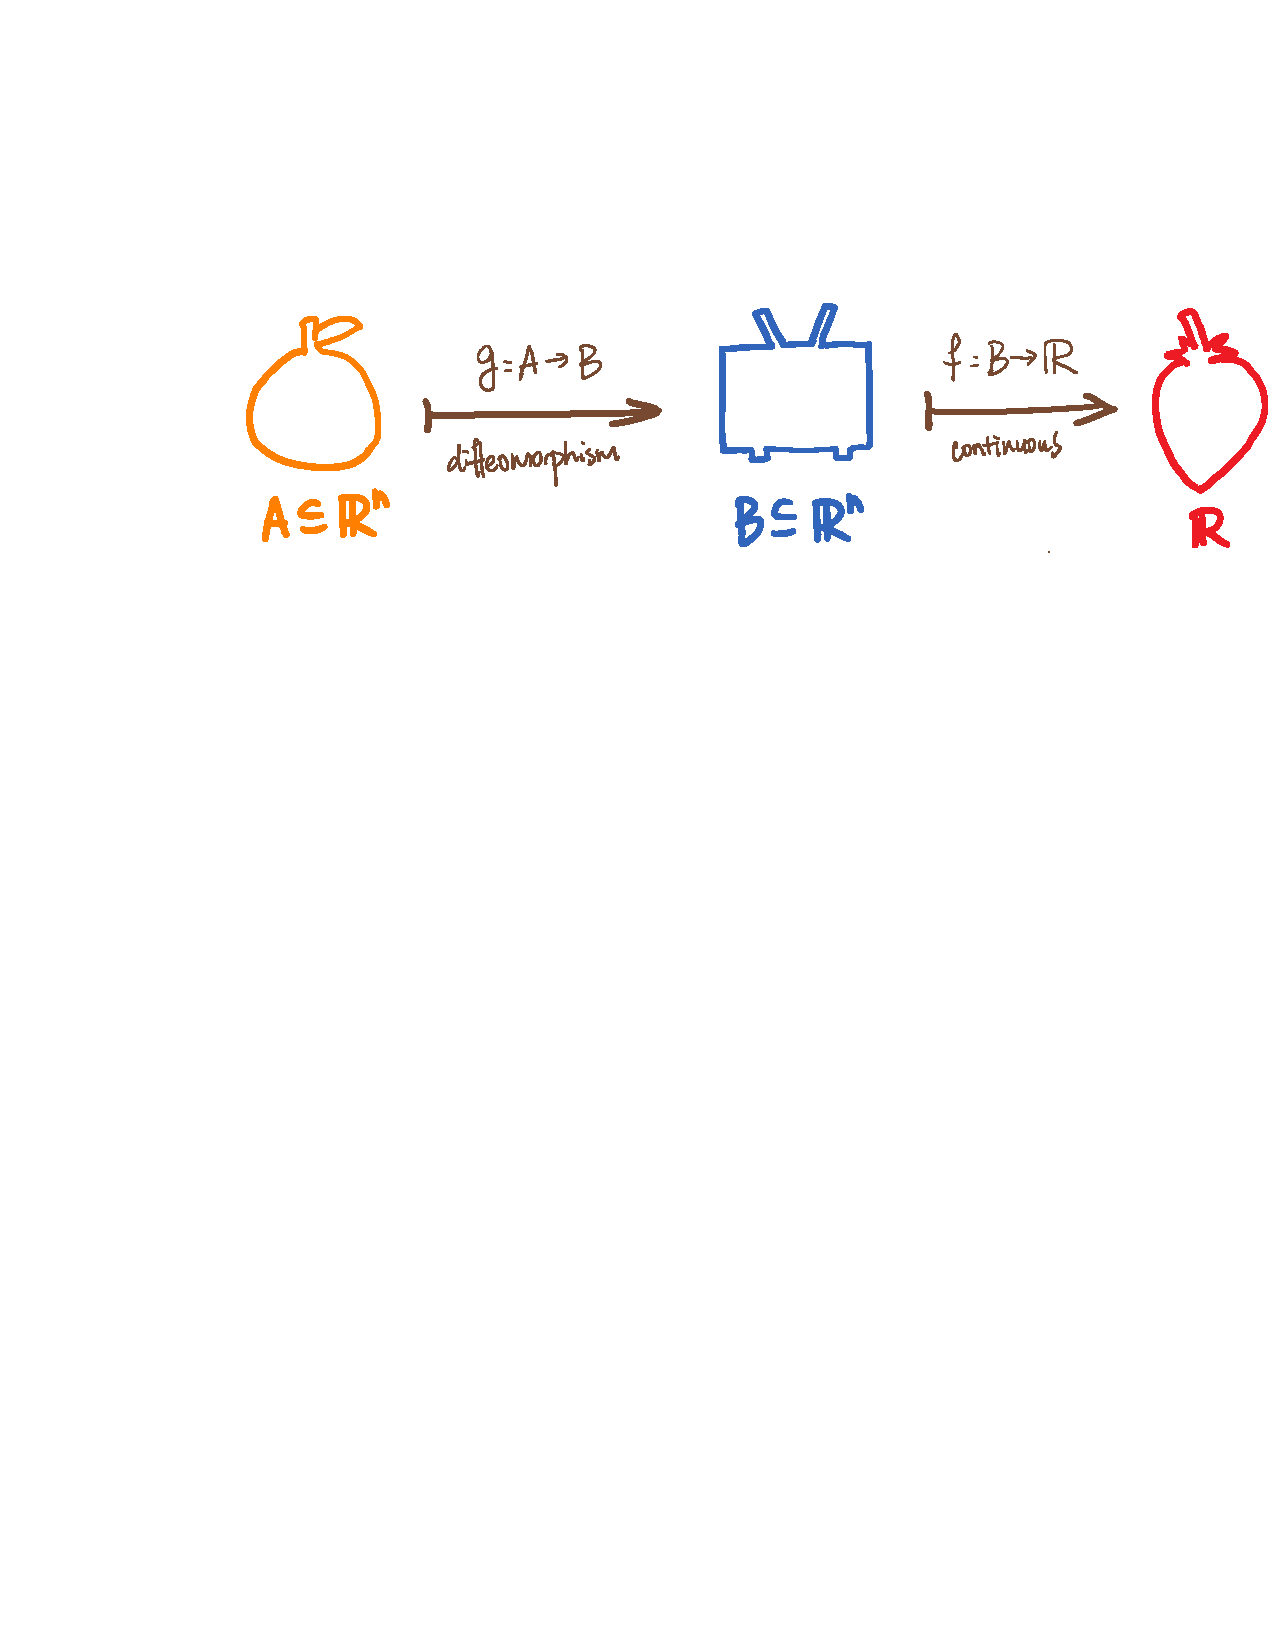
\includegraphics[scale=0.69]{chngOfVar.pdf}
\end{center}

\begin{defn}
Let $Q$ be a box in $\R^n$, and consider an affine map $T:\R^n \to \R^k \ \ \ \vec{x}\mapsto M\vec{x}+\vec{b}$ that maps $Q$ to $P$. $P$ is called a parallelepiped.  
\end{defn}
\note Given the settings in Definition 13.0.0.0.1, $P$ is rectifiable, with $V(P) = |\det(M)| \cdot V(Q)$.

\begin{defn}
Let $C$ be a compact rectifiable set in $\R^{n-1}$ for $n \geq 2$, let $\phi:C \to \R$ and $\psi:C \to \R$ be continuous functions such that $\phi(x) \leq \psi(x)$ for all $x \in C$. The set $S\coloneqq \{(x,t) \mid x \in C,\ \phi(x) \leq t \leq \psi(x)\}$ is called a simple region in $\R^n$. 
\end{defn}

\begin{lem}[Lemma 14.3 on Munkres]
Simple regions are compact and rectifiable.
\end{lem}

\begin{thm}[Fubini's Theorem for Simple Regions]
Let $S\coloneqq \{(x,t) \mid x \in C,\ \phi(x) \leq t \leq \psi(x)\}$ be a simple region in $\R^n$, where $C$ is a compact rectifiable set in $\R^{n-1}$ for $n \geq 2$, $\phi:C \to \R$ and $\psi:C \to \R$ are continuous functions with the property $\phi(x) \leq \psi(x)$ for all $x \in C$, let $f:S \to \R$ be a continuous function. Then $f$ is integrable over $S$ and we have the following holds: 
$$\int_S f = \int_{x \in C} \int_{t=\phi(x)}^{t=\psi(x)} f(x,t)\, dt\, dx$$
\end{thm}
\begin{proof}
The proof of this theorem is given by Theorem 14.4 on Munkres.
\end{proof}

\begin{thm}[Substitution Rule]
Let $I = [a,b]\subseteq \R$, let $g:I \to \R$ be a function of $C^1$ type, with $g'(x) \neq 0$ for all $x \in (a,b)$. Then the set $g(I)$ is a closed interval $J$ with end points $g(a)$ and $g(b)$. For continuous function $f:J \to \R$, we have the following holds:
$$\int_{g(a)}^{g(b)} f = \int_a^b (f\circ g) g'\qquad\qquad\qquad \int_J f = \int_I (f\circ g)|g'|$$
\end{thm}
\begin{proof}
The proof of this theorem is given by Theorem 17.1 on Munkres.
\end{proof}


\begin{thm}[Change of Variable Theorem]
Let $A$ be an open subset of $\R^n$, let $B$ be an open subset of $\R^n$, and let $g$ be a diffeomorphism from $A$ to $B$. For continuous function $f:B\to \R$, $f$ is integrable over $B$ if and only if the function $(f\circ g) \cdot |\det Dg|$ is integrable over $A$. Moreover, if $f$ is integrable over $B$, we have $$ext \int_B f = ext \int_A (f\circ g) \cdot |\det Dg|$$ 
That is, for continuous function $f:B \to \R$, we have either $ext \int_B f = ext \int_A (f\circ g) \cdot |\det Dg|$, or neither $ext \int_B f$ nor $ext \int_A (f\circ g) \cdot |\det Dg|$ exists.
\end{thm}

\note (The restriction of the Change of Variable Theorem on $\R$)\\
First we generalize the the Substitution Rule as a consequence of the Change of Variable Theorem:
Given the settings in Theorem 13.3, suppose we have $n=1$, and suppose further $A\subseteq \R$ is an open connected set, that is, we can write $A= (\alpha,\beta)$. In such case, the diffeomorphism $g$ defined on $A$ must be strictly monotonic, and we have either (1) $B = (g(\alpha),g(\beta))$,  or (2) $B = (g(\beta),g(\alpha))$. For case (1), we can write: $$ext \int_{(g(\alpha),g(\beta))} f = ext \int_{(\alpha,\beta)} (f\circ g)\cdot g'$$ 
For case (2), we have $$ext \int_{(g(\beta),g(\alpha))} f = -ext\int_{g(\alpha)}^{g(\beta)} f=- ext \int_{(\alpha,\beta)} (f\circ g)\cdot g' $$
These results follows immediately from the Substitution Rule, one can use Chain Rule and Fundamental Theorem of Calculus to prove these results easily.\\



\begin{proof}[Proof of Theorem 13.3]
\hfill\break
We start with some temporary added assumptions:
\begin{enumerate}[topsep=3pt,itemsep=-1ex,partopsep=1ex,parsep=1ex]
\item $A,B$ are bounded and rectifiable.
\item $g$ is a diffeomorphism from a neighborhood of $\bar{A}$ to neighborhood of $\bar{B}$
\item $f \in C(\bar{B},\R)$\\
\end{enumerate}

First we consider Special Case 1: \\
Suppose the function $g$ defined in the settings of Theorem 13.3 is a coordinate transposition that maps $(x_1,\cdots, x_l,\cdots,x_k,\cdots,x_n)$ to $(x_1,\cdots x_k, \cdots, x_l, \cdots, x_n)$. Then we know that $\det (Dg(\vec{x})) = -1 \Rightarrow |\det (Dg(\vec{x}))| =1$ for all $\vec{x}\in A$. Note that reorienting boxes does not alter their volume, then we can write:
$$\int_B f = \int_A f\circ g = \int_A (f\circ g)|\det(Dg)|$$ use extended integral when appropriate. This completes the proof of Theorem 13.3 for this Special Case 1. In this rest of the proof of Theorem 13.3, we will call such coordinate transposition function $g$ as Type-1 diffeomorphism.\\


Now consider Special Case 2: \\
Suppose the set $B$ defined in the settings of Theorem 13.3 is given by the following: 
$$B = \{ \vec{x}=(x_1,x_2,\cdots,x_n)\in \R^n\mid (x_1,\cdots, x_{n-1}) \in E, \phi(x_1,\cdots, x_{n-1}) < x_n < \psi(x_1,\cdots, x_{n-1})\}$$
where $E$ is a bounded open rectifiable subset of $\R^{n-1}$, and $\phi,\psi \in C(\bar{E}, \R)$ with $\phi(\vec{x}) < \psi(\vec{x}) $ for all $\vec{x}\in E$. Suppose further that the function $g$ defined in the settings of Theorem 13.3 maps $(x_1,x_2,\cdots, x_{n-1}, x_n)$ to $(x_1,\cdots, x_{n-1}, \alpha(\vec{x}))$, for some function $\alpha:A \to \R$. Here we can write: 
$$A = \{ \vec{x}\mid (x_1,\cdots,x_{n-1}) \in E , \phi(x_1,\cdots, x_{n-1}) < \alpha(\vec{x}) < \psi(x_1,\cdots,x_{n-1})\}$$
And we see that we get the followings:
\begin{enumerate}[topsep=3pt,itemsep=-1ex,partopsep=1ex,parsep=1ex]
\item $A$, $B$ are rectifiable by Lemma 14.3 on Munkres.
\item Given $\vec{x}' = (x_1,x_2,\cdots, x_{n-1}) \in E$, we see that: $$\vec{x}=(\vec{x}',x_n) \in A \iff x_n \text{ belongs to an interval determined by } \vec{x}'$$
\item Given $\vec{x}\in A$, we have $\det(Dg(\vec{x})) = D_n\alpha(\vec{x})$ because we have:
$$Dg(\vec{x})= \bmat{1&0&\cdots&0 \\ 0 & 1 & \cdots & 0 \\ \vdots &\vdots & &\vdots \\ D_1\alpha(\vec{x})& D_2\alpha(\vec{x}) &\cdots &D_n \alpha(\vec{x})}$$
\end{enumerate}

Let $\vec{x}' = (x_1,x_2,\cdots,x_{n-1})$ denote a vector in $E$, let $\vec{x} = (\vec{x}',x_n)$ denote a vector in $A$ determined by $\vec{x}'$, and let $I_{\vec{x}'}\subseteq \R$ denote the interval determined by $\vec{x}'$. By Fubini's Theorem on Simple Regions and Substitution Rule, one can write the following:
\begin{align*}
\int_B f &= \int_{\vec{x}' \in E} \int_{x_n \in (\phi(\vec{x}'), \psi(\vec{x}'))} f 
= \int_{\vec{x}' \in E} \int_{\alpha(\vec{x}) \in I_{\vec{x}'}} (f\circ g) |D_n\alpha|
= \int_A (f\circ g) |D_n\alpha| = \int_A (f\circ g) |\det Dg|
\end{align*}
This completes the proof of Theorem 13.3 for Special Case 2. In the rest of the proof of Theorem 13.3, we will call the function $g$ defined in Special Case 2 as Type-2 diffeomorphism. \\


\newpage
To proceed, we will make use of the following proposition:
\begin{prop}
\setlength{\leftskip}{1cm}Let $A,B,C$ be open subsets of $\R^n$, let $g:A \to B$ and $h:B \to C$ be diffeomorphisms, and let $f:C \to \R$ be a continuous function. If $f$ is integrable over $C$, and $f\circ h$ is integrable over $B$, then we have $\int_C f =\int_A (f\circ (h \circ g))| \det(D(h\circ g))|$. 
\end{prop}
\begin{proof}\setlength{\leftskip}{1cm}By the Change of Variable Theorem, one can write the following:
$$\qquad\qquad\int_C f = \int_B (f\circ h) |\det(D h)| = \int_A ((f\circ h) \circ g) |\det (Dh)| \cdot g |\det(Dg)| = \int_A f\circ h \circ g |\det (D(h\circ g))|$$
Use extended integral here when appropriate.
\end{proof}

Now suppose the function $g$ defined in the settings of Theorem 13.3 can be characterized by: $$g:A \to B \qquad\vec{x} =(x_1,\cdots,x_{j-1},x_j,x_{j+1},\cdots, x_n) \mapsto (x_1,\cdots, x_{j-1}, \eta(\vec{x}), x_{j+1},\cdots, x_n)$$
for some function $\eta:A \to \R$. Such diffeomorphism is called a generalized shear. In the rest of the proof of Theorem 13.3, we will call generalized shear as Type-3 diffeomorphism. Notice that, Type-3 diffeomorphisms can be obtained by compositions of of Type-1 and Type-2 diffeomorphism. Combing Proposition 13.3.1 with Special Case 1 and Special Case 2, it follows that the results of Theorem 13.3 holds for Type-3 diffeomorphism. Note that Type-1 diffeomorphism is a composition of two Type-3 diffeomorphism. Check Page 157 on Munkres for details.\\

The following proposition and theorem ensure that one can locally factorize any diffeomorphism into compositions of Type-1 and Type-2 diffeomorphism.

\begin{prop}\setlength{\leftskip}{1cm}
Any invertible affine map can be factored into composition of affine maps of Type-1 and Type-2, or equivalently, composition of Type-1 and Type-3.
\end{prop}
\begin{proof}\setlength{\leftskip}{1cm}
For linear maps, this follows from element matrix factorization from Theorem 2.4 on Munkres. For translation maps, one can move one coordinate at a time by using Type-3 diffeomorphism. All invertible affine maps can be obtained from composition of linear maps and translation maps. This completes the argument of this proposition.
\end{proof}

\begin{thm}[Theorem 18.3 on Munkres]\setlength{\leftskip}{1cm}
Let $A,B$ be open subset of $\R^n$, let $g:A \to B$ be a diffeomorphism, let $\vec{p}\in A$ with $g(\vec{p}) = \vec{q}\in B$. In some neighborhood of $\vec{p}$, the diffeomorphism $g$ can be factored into a composition of Type-1 diffeomorphisms and Type-2 diffeomorphisms. 
\end{thm}
\begin{proof}\setlength{\leftskip}{1cm}
Let $C$ denote the matrix $Dg(\vec{p})$. Since $g$ is a diffeomorphism, then by the Inverse Function Theorem, we know that $C$ is invertible. Define the following invertible affine maps:
$$\qquad\qquad t_1:\R^n \to \R^n\ \ \ \vec{x}\mapsto\vec{x}+\vec{p} \qquad\qquad t_2:\R^n \to \R^n \ \ \ \vec{x}-\vec{q}\qquad\qquad t_3:\R^n \to \R^n \ \ \ \vec{x}\mapsto C^{-1}\vec{x}$$
Now let $T_1=t_2^{-1}\circ t_3^{-1}$ and $T_2=t_1^{-1}$, we get the followings:
\begin{enumerate}[topsep=3pt,itemsep=-1ex,partopsep=1ex,parsep=1ex,leftmargin=1.5cm]
\item $\hat{g} \coloneqq T_1^{-1} \circ g \circ T_2^{-1}$ is a diffeomorphism, $g = T_1 \circ \hat{g} \circ T_2$.
\item $T_2(\vec{p}) = \vec{0}$, and $T_1(\vec{0}) = \vec{q}$
\item $D\hat{g}(\vec{0}) = I $, where $I$ is the $n \times n$ identity matrix.
\end{enumerate}
From (2), we get $\hat{g}(\vec{0}) = \vec{0}$. \\
From (3), we get $D\hat{g}_k(\vec{0}) = \vec{e}_k^T$.\\
From Chain Rule, we get $DT_1= Dg(\vec{p})$ and $DT_2 = I$. \\ 
Now we define the following maps:
\begin{align*}
\qquad\qquad
\bmat{x_1\\x_2\\x_3\\\cdots,\\x_n} \mapsto \bmat{\hat{g}_1(\vec{x})\\x_2\\x_3\\\cdots \\x_n} \qquad\qquad
\bmat{x_1\\x_2\\x_3\\\cdots,\\x_n}\mapsto \bmat{\hat{g}_1(\vec{x})\\\hat{g}_2(\vec{x})\\x_3\\\cdots\\ x_n} \qquad\qquad
\cdots \qquad\qquad
\bmat{x_1\\x_2\\x_3\\\cdots,\\x_n} \mapsto \hat{g}(\vec{x})
\end{align*}
By the Inverse Function Theorem, each of these maps is a diffeomorphism in some neighborhood of $\vec{0}$ because the derivative of each of them at $\vec{0}$ is $I$. We observe that each of these maps is a Type-3 diffeomorphism. Then we get an induced map given by the following:
$$\qquad\qquad\bmat{x_1\\x_2\\x_3\\\cdots,\\x_n} \mapsto \bmat{\hat{g}_1(\vec{x})\\x_2\\x_3\\\cdots \\x_n} \mapsto \bmat{\hat{g}_1(\vec{x})\\\hat{g}_2(\vec{x})\\x_3\\\cdots\\ x_n} \mapsto
\cdots \mapsto \hat{g}(\vec{x})$$
Combining with Proposition 13.3.2, the result follows.
\end{proof}

Concluding the above, we have got a local version of Theorem 13.3. To finish the proof of Theorem 13.3, we will need the Partition of Unity Theorem to partition the function $f$ on the open set $B$.

\begin{defn}
Let $X$ be a metric space, and let $V$ be a vector space, let $f:X \to V$. \\
The support of $f$, denoted as $supp(f)$, is defined to be the closure of the set $\{\vec{x}\mid f(\vec{x}) \neq \vec{0}\}$ in $X$.
\end{defn}

\note Let $X$ be a metric space, and let $V$ be a vector space, let $f:X \to V$. \\For $\vec{x}\in X$, $\vec{x}\notin supp(f)$ if and only if $\exists\ \epsilon > 0$ such that $f(\vec{t}) = \vec{0}$, $\forall \vec{t}\in B_\epsilon(\vec{x})$. 

\begin{corT}\setlength{\leftskip}{1cm}
Let $A,B$ be open subset of $\R^n$, let $g:A \to B$ be a diffeomorphism, let $\vec{p}\in A$ with $g(\vec{p}) = \vec{q}\in B$. There exists some open neighborhood $U$ of $\vec{p}$, and some open neighborhood $V$ of $\vec{q}$ such that $g|_U:U \to V$ defines a diffeomorphism that can be factored into Type-1 and Type-2 diffeomorphisms. For some continuous function $f:B \to \R$, if $supp(f) \subseteq U$, then we have either $ext \int_B f = ext \int_A (f\circ g) \cdot |\det Dg|$, or neither $ext \int_B f$ nor $ext \int_A (f\circ g) \cdot |\det Dg|$ exists.
\end{corT}

\begin{center}
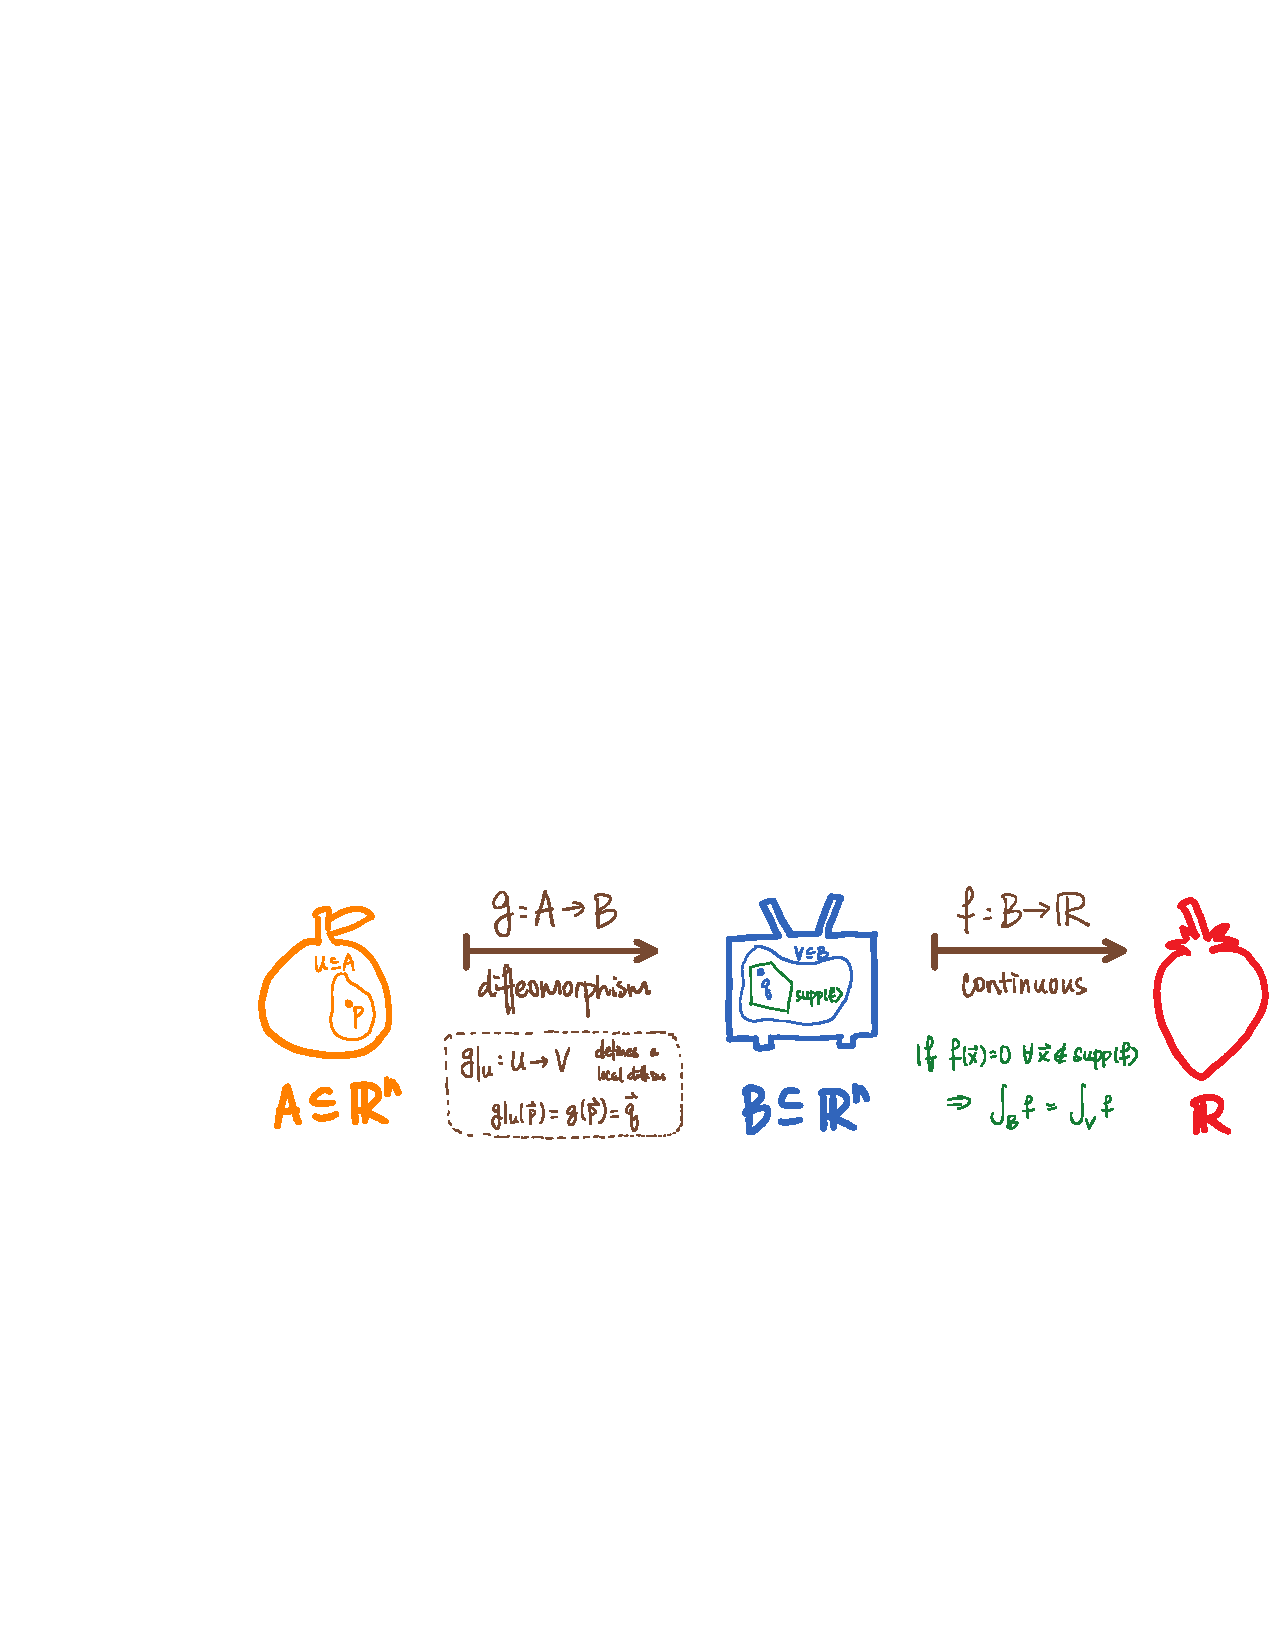
\includegraphics[scale=0.69]{cor13.4.pdf}
\end{center}

The Partition of Unity Theorem gives us a way to partition the function $f$ on the open set $B$ such that the support of each partition of $f$ is contained in some desired open subset of $B$, in which case we can apply Corollary 13.4.1 to complete the proof of the Change of Variable Theorem.

\begin{lem}
\setlength{\leftskip}{1cm}The function $f$ given by the following belongs to $C^\infty (\R,[0,\infty))$: $$f:\R \to \R \ \ \ \begin{cases}e^{-1/x} &x>0\\0&x\leq 0  \end{cases}$$
\end{lem}
\begin{proof}
\setlength{\leftskip}{1cm}The proof of this lemma is given in Spivak Chapter 18.
\end{proof}

\begin{corL}
\setlength{\leftskip}{1cm}Consider the function: 
$$f:\R \to \R \ \ \ \begin{cases}e^{-1/x} &x>0\\0&x\leq 0  \end{cases}$$
For $Q = [a_1,b_1]\times [a_2,b_2] \times \cdots \times [a_n,b_n]$, the function $\Phi_Q(\vec{x}) = f(x_1-a_1)f(b_1-x_1)\cdots f(x_n-a_n)$ is in $C^\infty(\R^n,[0,\infty))$, with $supp(\Phi_Q) = Q$ and $\Phi_Q (\vec{x})> 0$ for all $\vec{x}\in Q$. 
\end{corL}


\begin{lem}
\setlength{\leftskip}{1cm}One can find positive volume boxes $Q_1,Q_2,\cdots$ such that the following holds:
\begin{enumerate}[topsep=3pt,itemsep=-1ex,partopsep=1ex,parsep=1ex,leftmargin=1.5cm]
\item $\Omega = \bigcup_j Int(Q_j)$
\item Each $Q_j$ is contained in some $U_{\alpha_j}$
\item Each $y \in \Omega$ has neighborhood meeting only finitely many $Q_j$, such property is called the local finiteness 
\end{enumerate} 
\end{lem}
\begin{proof}
\setlength{\leftskip}{1cm}Write $\Omega = K_1 \cup K_2\cup \cdots$ with each $K_j$ being compact, and $K_j \subseteq Int(K_{j+1})$. Check Lemma 15.1, or a previous theorem in this text. Letting $E_j = K_j \setminus Int(K_{j-1})$, each $E_j$ is compact, and disjoint from $K_{j-2}$ for $j \geq 3$. $E_j \subseteq Int(\hat{Q}_{j,1}) \cup \cdots \cup Int(\hat{Q}_{j,M_j})$, with each $\hat{Q}_{j,k}$ contained in some $U_\alpha$, and each $\hat{Q}_{j,k}$ is disjoint from $K_{j-2}$. Then we can write $\Omega = \bigcup_{j,k} Int(\hat{Q}_{j,k})$. $K_j$ meets at most $M_{i} + \cdots + M_j$ of the $\hat{Q}_{j,k}$. Relabel the $\hat{Q}_{j,k}$ as $Q_1,Q_2,Q_3,\cdots$ This completes the proof of the lemma. 
\end{proof}

Now we have got our setup for the Partition of Unity Theorem.

\newpage
\begin{thm}[Partition of Unity Theorem]
\setlength{\leftskip}{1cm}Let $\Omega$ be an open subset of $\R^n$. If $\Omega = \bigcup_{\alpha \in A} U_\alpha$ for some open subsets $U_\alpha$ of $\R^n$, then there exist some functions $\phi_1,\phi_2,\cdots \in C^\infty(\Omega, [0,\infty))$ such that the followings hold:
\begin{enumerate}[topsep=3pt,itemsep=-1ex,partopsep=1ex,parsep=1ex,leftmargin=1.5cm]
\item Each $supp(\phi_j)$ is compact
\item Each $supp(\phi_j)$ is contained in some $U_\alpha$
\item Each $\vec{x}\in \Omega$  has an open neighborhood that intersects only finitely many $supp(\phi_j)$
\item $\sum_{j=1}^\infty \phi_j(\vec{x}) = 1$ for all $\vec{x}\in \Omega$, such sum is called the locally finite sum.
\end{enumerate}
\end{thm}
\begin{proof}\setlength{\leftskip}{1cm}
The proof of this theorem follows from the Fundamental Theorem of Laziness.\\ Section 16 on Munkres gives a proof for this theorem. Alternatively, consider the following:
Let $\Phi(Q_i)$ be functions defined appropriately similar to those given in Corollary 13.4.2.1. Let $\lambda$ be a function defined by $\lambda(\vec{x}) = \sum_{j=1}^\infty \Phi_{Q_j}(\vec{x})$. Here we have $\lambda \in C^\infty(\Omega,(0,\infty))$, and the following holds: $$1 = \sum_{j=1}^\infty \frac{\Phi_{Q_j}(\vec{x})}{\lambda(\vec{x})} $$ We let $\phi_j(\vec{x}) \coloneqq \frac{\Phi_{Q_j}(\vec{x})}{\lambda(\vec{x})}$, which is a $C^\infty$ function, and we have $supp(\phi_j) =Q_j$. Then the results of Theorem 13.5 follow immediately. 
\end{proof}

\begin{lem}\setlength{\leftskip}{1cm}
Let $B$ be an open subset of $\R^n$, let $f \in C(B ,\R)$ such that $ext\int_B f$ exists, let $(\phi_j)$ be a sequence of functions in $C^\infty(B,[0,\infty])$ that satisfies conditions (1),(3),(4) in the Partition of Unity Theorem. Then we can write $ext\int_B f = \sum_{j =1}^\infty \int_B \phi_j \cdot f$.
\end{lem}
\begin{proof}\setlength{\leftskip}{1cm}
First we will tackle the case where $f\geq 0$, then apply to $f_+$ and $f_-$ and combine the results. Assume that $f \geq 0$, suppose $E$ is a compact rectifiable subset of $B$. Then there exists $M$ such that $\phi_j = 0$ on $E$ for $j \geq M$. Since $f \geq 0$, here we have:
$$\int_E f = \int_E \sum_{j=1}^\infty \phi_j\cdot f = \int_E \sum_{j=1}^M \phi_j \cdot f = \sum_{j=1}^M \int_E \phi_j \cdot f  \leq \sum_{j=1}^M \int_B \phi_j \cdot f \leq \sum_{j=1}^\infty \int_B \phi_j \cdot f$$
Take the supremum over $E$, and get the following:
$$ext \int_B f \leq \sum_{j=1}^\infty \int_B \phi_j \cdot f$$
On the other hand, we have the following:
$$\sum_{j=1}^\infty \int_B \phi_j\cdot f = \lim_{M \to \infty} \sum_{j=1}^M \int_B \phi_j\cdot f = \lim_{M\to \infty} \int_B \sum_{j=1}^M \phi_j f \leq ext\int_B f$$
Combine the two inequalities and apply to $f_+$ and $f_-$ to get the result for this Lemma.
\end{proof}

Combining the results from above to complete the proof of Theorem 13.3:\\

For $\vec{y}\in B$, choose an open subset $U_{\vec{y}}$ of $B$ such that $g$ can be factorized into Type-1 and Type-2 diffeomorphisms on $U_{\vec{y}}$, then choose a partition of unity $(\phi_j)$ dominated by $\{U_{\vec{y}} \mid \vec{y}\in B \}$. Now we can write the following:
$$ext\int_B f_+ = \sum_{j=1}^\infty \int_A (\phi_j \circ g) (f_+\circ g) |\det Dg| = ext \int_A (f_+\circ g)|\det Dg| $$
$$ext\int_B f_- = \sum_{j=1}^\infty \int_A (\phi_j \circ g) (f_-\circ g) |\det Dg| = ext \int_A (f_-\circ g)|\det Dg| $$
Combining the results for $f_+$ and $f_-$ to get the desired results for Theorem 13.3.
\end{proof}


\note In the settings of Theorem 13.3, suppose we have $g :A \to B \ \ \  \vec{x}\mapsto r \vec{x}$ for some $r >0$.
$$ext \int_{\vec{x}\in B} f(\vec{x}) = ext\int_{\vec{x}\in A} f(r\vec{x})\cdot r^n$$

\newpage
\begin{defn}
The number $\pi$ is defined to be the following:
$$\pi \coloneqq \lambda_2 \coloneqq V(B_1^2(\vec{0}))$$
\end{defn}

\hfill\break

\example Let $B_r^n(\vec{0}) \coloneqq \{ \vec{x}\in \R^n \mid ||\vec{x}|| <r\}$, we have $V(B_r^n(\vec{0})) = r^n V(B_1^n(\vec{0})) \coloneqq r^n\lambda_n$.\\


\example We have $\frac{V(B_1^n(\vec{0}))}{V([-1,1]^n)} \leq 1$.
\begin{align*}
\lambda_n = \int_{B_1^n(\vec{0}))} 1 = \int_{\vec{x}\in B_1^k (\vec{0})} \int_{\vec{y}\in B_{\sqrt{1-||\vec{x}||^2}}^{n-k}} 1 = \int_{\vec{x}\in B_1^k(\vec{0})} \left(1-||\vec{x}||^2\right)^{\frac{n-k}{2}} \lambda_{n-k} 
\end{align*}
Here we choose $k=2$, then we can rewrite:
\begin{align*}
\lambda_n &= \lambda_{n-2} \int_{B_1^2(\vec{0})} (1-||\vec{x}||^2)^{\frac{n}{2}-1} \\&= \lambda_{n-2} \int_{B_1^2(\vec{0})\setminus ((-1,0]\times \{0\})} (1-||\vec{x}||^2)^{\frac{n}{2}-1} + \lambda_{n-2} \int_{(-1,0]\times \{0\}} ( 1-||\vec{x}||^2)^{\frac{n}{2}-1}
\end{align*}
Here $\lambda_{n-2} \int_{(-1,0]\times \{0\}} ( 1-||\vec{x}||^2)^{\frac{n}{2}-1} = 0$ by Theorem 11.13 from Munkres. Let $g:\R^2 \to \R^2 \ \ \ (r,\theta) \mapsto (r\cos(\theta),r\sin(\theta))$. Notice that $g$ is a local diffeomorphism and $\det Dg(r,\theta) = r$.  
\begin{align*}
\lambda_n &=  \lambda_{n-2} \int_{B_1^2(\vec{0})\setminus ((-1,0]\times \{0\})} (1-||\vec{x}||^2)^{\frac{n}{2}-1} \\
&= \lambda_{n-2} \int_{\{r \mid 0<r<1\}\times \{\theta \mid -\pi<\theta <\pi\}} (1-r^2)^{\frac{n}{2}-1} r\\
&= \lambda_{n-2} \int_0^1 \int_{-\pi}^\pi (1-r^2)^{\frac{n}{2}-1} r\, d\theta\, dr\\
&= 2 \pi \lambda_{n-2} \int_0^1 (1-r^2)^{\frac{n}{2}-1} r\, dr\\
&= \pi \lambda_{n-2} \int_{0}^1 t^{\frac{n}{2}-1}\, dt \\
&= \frac{2\pi\lambda_{n-2}}{n}
\end{align*}
with $t =1-r^2$ and $dt = 2r\, dr$. It follows that, for $u \in \N$, we have: $$\lambda_{2u} = \frac{\pi^u}{u!} \qquad\qquad\qquad\lambda_{2u+1} = \frac{2^{u+1}\pi^u}{(2u+1)(2u-1)(2u-3)\cdots(3)(1)}$$

\exercise
For $n \in \N$, let $\mu_n = V([-1,1]^n) = 2^n$, and let $\kappa_n$ be defined as:
$$\kappa_n = V\left(\left\{\vec{x}=(x_1,x_2,\cdots,x_n)\in \R^n \left|\  \sum_{i=1}^n|x_i| < 1 \right.\right\} \right)= \frac{2^n}{n!}$$
We get $\kappa_n \leq \lambda_n \leq \mu_n$, $\lim_{n\to \infty} \frac{\lambda_n}{\mu_n} = 0$, and $\lim_{n \to \infty} \frac{\kappa_n}{\lambda_n}= 0$. \\

\exercise Let $\Omega$ be a rectifiable subset of $\R^n$, let $h$ be an isometry that maps $\Omega$ to $h(\Omega)$, we have: $$V(h(\Omega)) = \int_{h(\Omega)} 1 = \int_{\Omega} 1\cdot |\det Dh| = V(\Omega)$$

\newpage
\begin{defn}
Let $A$ be a rectifiable subset of $\R^n$ with positive volume, let $f:A \to \R$ be an integrable function. $${avg}_A f = \frac{\int_A f}{V(A)}$$
\end{defn}
\note In the setting of Definition 13.5.1.0.2, we have $\inf_A f \leq {avg}_A f \leq \sup_A f$.\\

\begin{defn}
Let $A$ be a rectifiable subset of $\R^n$, and let $f:A\to \R^n \ \ \ \vec{x} \mapsto (f_1(\vec{x}),f_2(\vec{x}),\cdots, f_n(\vec{x}))$ be an integrable function. $$\int_A f \coloneqq \bmat{\int_A f_1 \\ \int_A f_2 \\ \vdots \\ \int_A f_n}$$
\end{defn}
\note In the settings of Definition 13.5.1.0.3, we have the following holds: 
$$avg_A f\coloneqq \frac{\int_A f}{V(A)}\in \R^n$$ 
and for a special case where $f:\R^n \to \R^n \ \ \ \vec{x}\mapsto \vec{x}$, $avg_A f$ is called the centroid of $A$. \\
Here we can write:
$$avg_A f = \bmat{avg_A \,f_1 \\ avg_A \, f_2 \\ \vdots \\ avg_A \, f_n}$$

\remark The height of the centroid of the upper half of a unit sphere is greater than the height of the centroid of the upper half of a unit ball.\\



\newpage
\section[Volume of Parallelopipeds]{\color{red} Volume of Parallelopipeds \color{black}}

\begin{defn}
Let $Q$ be a box in $\R^k$, and let $T$ be an affine injection from $\R^k$ to $\R^n$ of the form $T(\vec{x}) = A\vec{x}+\vec{b}$ for some matrix $A$ and $\vec{b}\in \R^n$. $T(Q)$ is called a $k$-parallelopiped.
\end{defn}

For $k<n$, let $Q$ be a box in $\R^k$, and let $T$ be an affine injection from $\R^k$ to $\R^n$ of the form $\vec{x}\mapsto A\vec{x}+\vec{b}$ for some matrix $A$ and vector $\vec{b}\in \R^n$. $T(Q)$ is a $k$-parallelopiped. Here we note that the $n$-volume of the $k$-parallelopiped $T(Q)$ is always zero because $T(Q)$ lies in a $k$-dimensional subspace of $\R^n$ which has measure zero. We want to find a way to define the $k$-volume of $T(Q)$, denoted as $V_k(T(Q))$. Here are some expectations for such definition: 
\begin{enumerate}[topsep=3pt,itemsep=-1ex,partopsep=1ex,parsep=1ex]
\item In the case where $A = \bmat{M \\ Z}$ for some $k\times k$ matrix $M$ and zero matrix $Z$, we should have $$V_k(T(Q))= |\det M|\cdot V(Q)$$
\item For isometry $h:\R^n \to \R^n$, we should have $V_k(h(T(Q))) = V_k(T(Q))$
\end{enumerate}


\hfill\break
\begin{thm}[Theorem 21.2 from Munkres] 
For $k\leq n$, let $T:\R^k \to \R^n \ \ \ \vec{x} \mapsto A\vec{x}+\vec{b}$ be an affine injection for some matrix $A$ and $\vec{b}\in \R^n$.\\ One can pick an orthogonal $n \times n$ matrix $B$ such that we have: $$B\cdot A= \bmat{M \\ Z}$$ for some $k\times k$ matrix $M$ and zero matrix $Z$.
\end{thm}
\begin{proof}
First $k$ rows of $B$ forms an orthonormal basis for column space of $A$. Extend such orthonormal basis to an orthonormal basis of $\R^n$ to obtain the remaining rows of $B$ by applying the Gram-Schmidt Process. 
\end{proof}


Given the settings in Theorem 14.1, we have $(BA)^T = \bmat{M& Z}$, and $(BA)^T (BA) = M^TM$. Now let $h:\R^n \to \R^n \ \ \ \vec{y}\mapsto B\vec{y}$, note that $h$ is an isometry, and we have the following being satisfied:
\begin{align*}
V_k(T(Q)) = V_k(h(T(Q))) &= |\det(M)|\cdot V(Q) \\&= \sqrt{\det(M^TM)}\cdot V(Q) \\&= \sqrt{\det((BA)^T(BA))}V(Q) \\&= \sqrt{\det(A^TA)}\cdot V(Q)
\end{align*}

\begin{lem}
Let $A$ be an $n \times k$ matrix, we have $\ker(A^TA) = \ker(A)$
\end{lem}
\begin{proof}
It is trivial that we have $\ker(A) \subseteq \ker(A^TA)$. On the other hand, if $A^TA\vec{x}=0$ for some $\vec{x}$, then $||A\vec{x}||^2=\left<A\vec{x}, A\vec{x}\right>= \vec{x}^TA^TA\vec{x} = 0 \Rightarrow A\vec{x} = \vec{0}$. This shows that $\ker(A^TA)\subseteq \ker(A)$.
\end{proof}

\begin{corL}
Let $A$ be an $n \times k$ matrix, then $rank(A^TA) = k-\dim(\ker(A^TA))=k-\dim(\ker(A)) = rank(A)$. 
\end{corL}

\begin{corL}
Let $A$ be an $n \times k$ matrix. If $k>n$, then $\det(A^TA) = 0$. 
\end{corL}
\begin{proof}
$k>n$ implies $rank(A) \leq n <k$, which implies $rank(A^TA)<k$, hence $\det(A^TA) = 0$.
\end{proof}

\begin{corL}
Let $A$ be an $n \times k$ matrix. If $k<n$, then $\det(AA^T) = 0$.
\end{corL}

\begin{lem}
Let $A$ be an $n \times k$ matrix. We have $A^TA\geq 0$.
\end{lem}
\begin{proof}
For $\vec{x}$, we have $\vec{x}^TA^TA\vec{x} = \left<A\vec{x},A\vec{x}\right>\geq 0$.
\end{proof}

\begin{corL}
Let $A$ be an $n \times k$ matrix. All eigenvalues of $A^TA$ are greater than or equal to $0$.
\end{corL}

\begin{corL}
Let $A$ be an $n \times k$ matrix, $\det(A^TA) \geq 0$. 
\end{corL}

\begin{defn}
Let $Q$ be a box in $\R^k$, and let $T$ be an affine injection from $\R^k$ to $\R^n$ of the form $\vec{x}\mapsto A\vec{x}+\vec{b}$ for some matrix $A$ and vector $\vec{b}\in \R^n$. We define $V_k(T(Q)) = \sqrt{\det(A^TA)}\cdot V(Q)$. 
\end{defn}

In the following discussion, we will show that the $k$-volume of a parallelopied defined in Definition 14.1.2.2.1 is legitimate. Let $Q_1$ be a box in $\R^k$, and let $T_1$ be an affine injection from $\R^k$ to $\R^n$ of the form $\vec{x}\mapsto A_1\vec{x}$ for some matrix $A_1$.\\

First check independent of choices. Suppose $T_1(Q_1)$ can also be obtained by a composition of affine maps $T_2$ and $C$, $T_1(Q_1) = T_2(C(Q_1))$. Here $C$ is a diffeomorphism. \\
\begin{center}
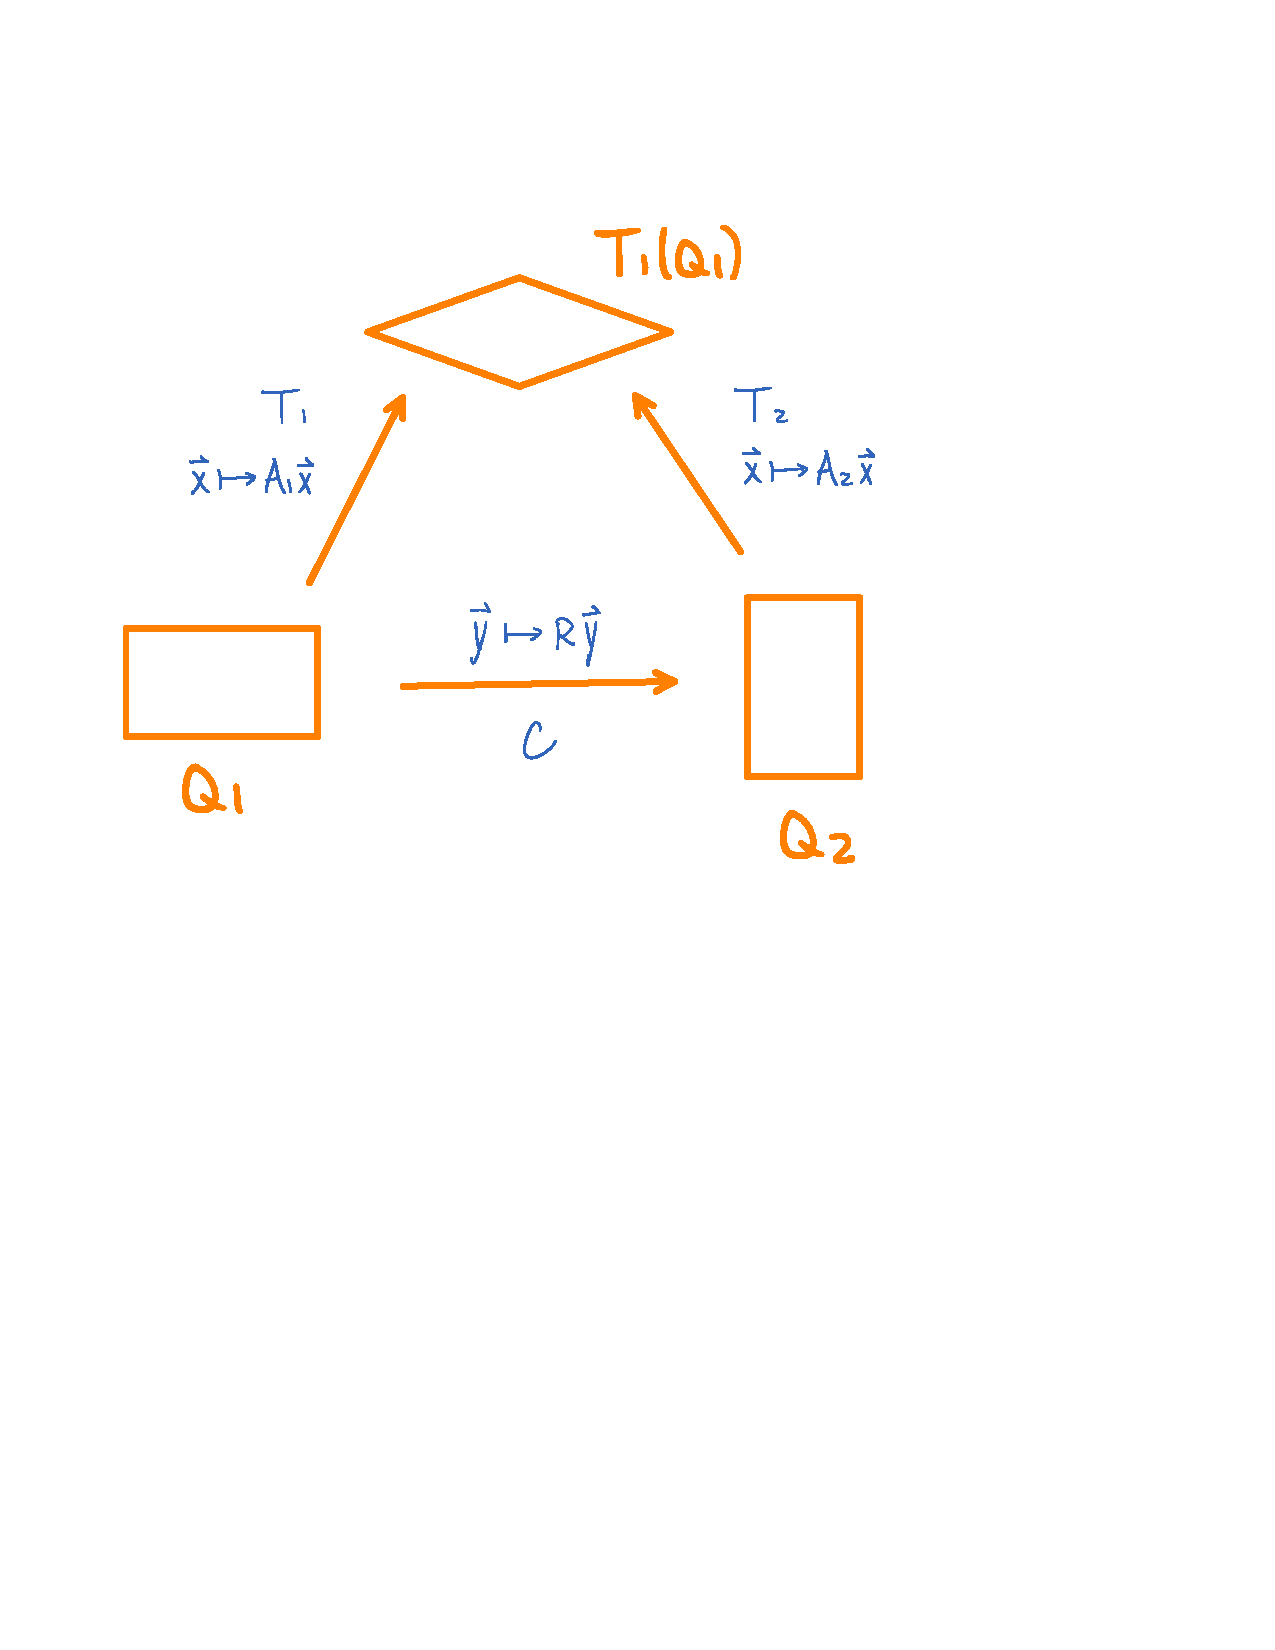
\includegraphics[scale=0.5]{parallpied.pdf}
\end{center}
Let $A_1$ denote the matrix for $T_1$, and let $A_2$ denote the matrix for $T_2$. Here we have $A_1 = A_2 R$:
\begin{align*}
\sqrt{\det(A_1^TA_1)} \cdot V(Q_1) &= \sqrt{\det((A_2R)^T(A_2R))} \cdot V(Q_1) \\&= \sqrt{\det(R^TA_2^TA_2R)} \cdot V(Q_1) \\&= \sqrt{\det(R^T)\det(A_2^TA_2)\det(R)}\cdot V(Q_1) \\&= \sqrt{\det(A_2^TA_2)}\cdot |\det(R)|\cdot V(Q_1) \\&= \sqrt{\det(A_2^TA_2)}\cdot V(Q_2)
\end{align*}
This shows that the $k$-volume of $T_1(Q_1)$ is well-defined. Now we will check the expectations for the definition of $k$-volume of a parallelopiped:
\begin{enumerate}[topsep=3pt,itemsep=-1ex,partopsep=1ex,parsep=1ex]
\item If $A_1 = \bmat{M \\ Z}$ for some $k\times k$ matrix $M$ and zero matrix $Z$, $V_k(T_1(Q_1))= |\det M|\cdot V(Q_1)$.
\item For isometry $h:\R^n \to \R^n$, we should have $V_k(h(T(Q))) = V_k(T(Q))$.
\end{enumerate}
For expectation (1). Suppose we have $A_1 = \bmat{M&Z}^T$, then we see that $\sqrt{\det(A_1^TA_1)} = \sqrt{\det(M^TM)} = |\det(M)|$, which implies $V_k(T_1(Q_1)) = |\det(M)| V(Q_1)$. For  expectation (2). Consider an isometry $h:\vec{x}\mapsto B\vec{x}+\vec{p}$ for some orthogonal matrix $B$, we see that $\det((BA_1)^T(BA_1)) = \det(A_1^TA_1)$, hence it follows that $V_k(h(T_1(Q_1))) = V_k(T_1(Q_1))$.\\

So we see that there exists a map 
$V_k: \{k-\text{parallelopipeds}\}\mapsto (0,\infty)$ that satisfies expectation (1) and expectation (2) that can define the $k$-volume of a parallelopiped, given by the following:
$$V_k(T(Q)) = \sqrt{\det(A^TA)}\cdot V(Q)$$

\begin{defn}
Let $A$ be an $n \times k$ matrix. $\mathcal{V}(A) \coloneqq \sqrt{\det(A^TA)}$
\end{defn}

\begin{thm}[Pythagorean Theorem]
For $n\geq k$, let $A$ be an $n \times k$ matrix. \\
$(\mathcal{V}(A))^2=$ the sum of the squares of the determinant of $k \times k$ sub-matrices of $A$. 
\end{thm}
\begin{proof}
The proof of this theorem is given in Theorem 21.4 on Munkres.
\end{proof}

\begin{corT}
Let $\vec{a}=(a_1,a_2,\cdots,a_n),\vec{b}=(b_1,b_2,\cdots,b_n)\in \R^n$. \\$$\left[\text{the one dimensional volume of the line segment from }\vec{a}\text{ to }\vec{b}\right]^2 = \sum_{j=1}^n (b_j - a_j)^2$$
\end{corT}
\begin{proof}
Proceed by using the affine map $f:[0,1] \to \R^n \ \ \ t\mapsto t(\vec{b}-\vec{a})+\vec{a}$. 
\end{proof}

\newpage
\chapter{Manifolds}
\setcounter{section}{14}
There are three kinds of non-affine $k$-dimensional objects. 
\begin{enumerate}[topsep=3pt,itemsep=-1ex,partopsep=1ex,parsep=1ex]
\item Parametrized $k$-manifold, discussed in section 22 on Munkres
\item $k$-manifold in $\R^n$, discussed in section 23 on Munkres
\item Abstract $k$-manifold, discussed in section 41 on Munkres
\end{enumerate} 

\section[Parametrized Manifolds]{\color{red} Parametrized Manifolds \color{black}}

\begin{defn}
Let $k,n,r\in \N$ with $k \leq n$, let $\alpha \in C^r(U, \R^n)$, where $U$ is an open subset of $\R^k$.  The set $Y \coloneqq \alpha(U)$, equipped with the map $\alpha$, constitute a parametrized $k$-manifold of class $C^r$, denoted as $Y_\alpha$. The $k$-volume of $Y_\alpha$ is defined by the following:
$$V_k(Y_\alpha) \coloneqq ext \int_U \mathcal{V}(D\alpha)$$
\end{defn}

\remark In the settings of Definition 15.0.0.0.1, for a special case where we have $k=n$, we will have $\mathcal{V}(D\alpha) = |\det D\alpha|$. Suppose further $Y$ is an open rectifiable subset of $\R^n$, and $\alpha:U \to Y$ is a diffeomorphism, then we have: 
$$V_n(Y_\alpha) = \int_U|\det (D\alpha)| = \int_Y 1 = V(Y)$$
In such case, we consider an example where $U = (0,1) \times (0,3\pi)$, and $\alpha$ defined by the following:
\begin{center}
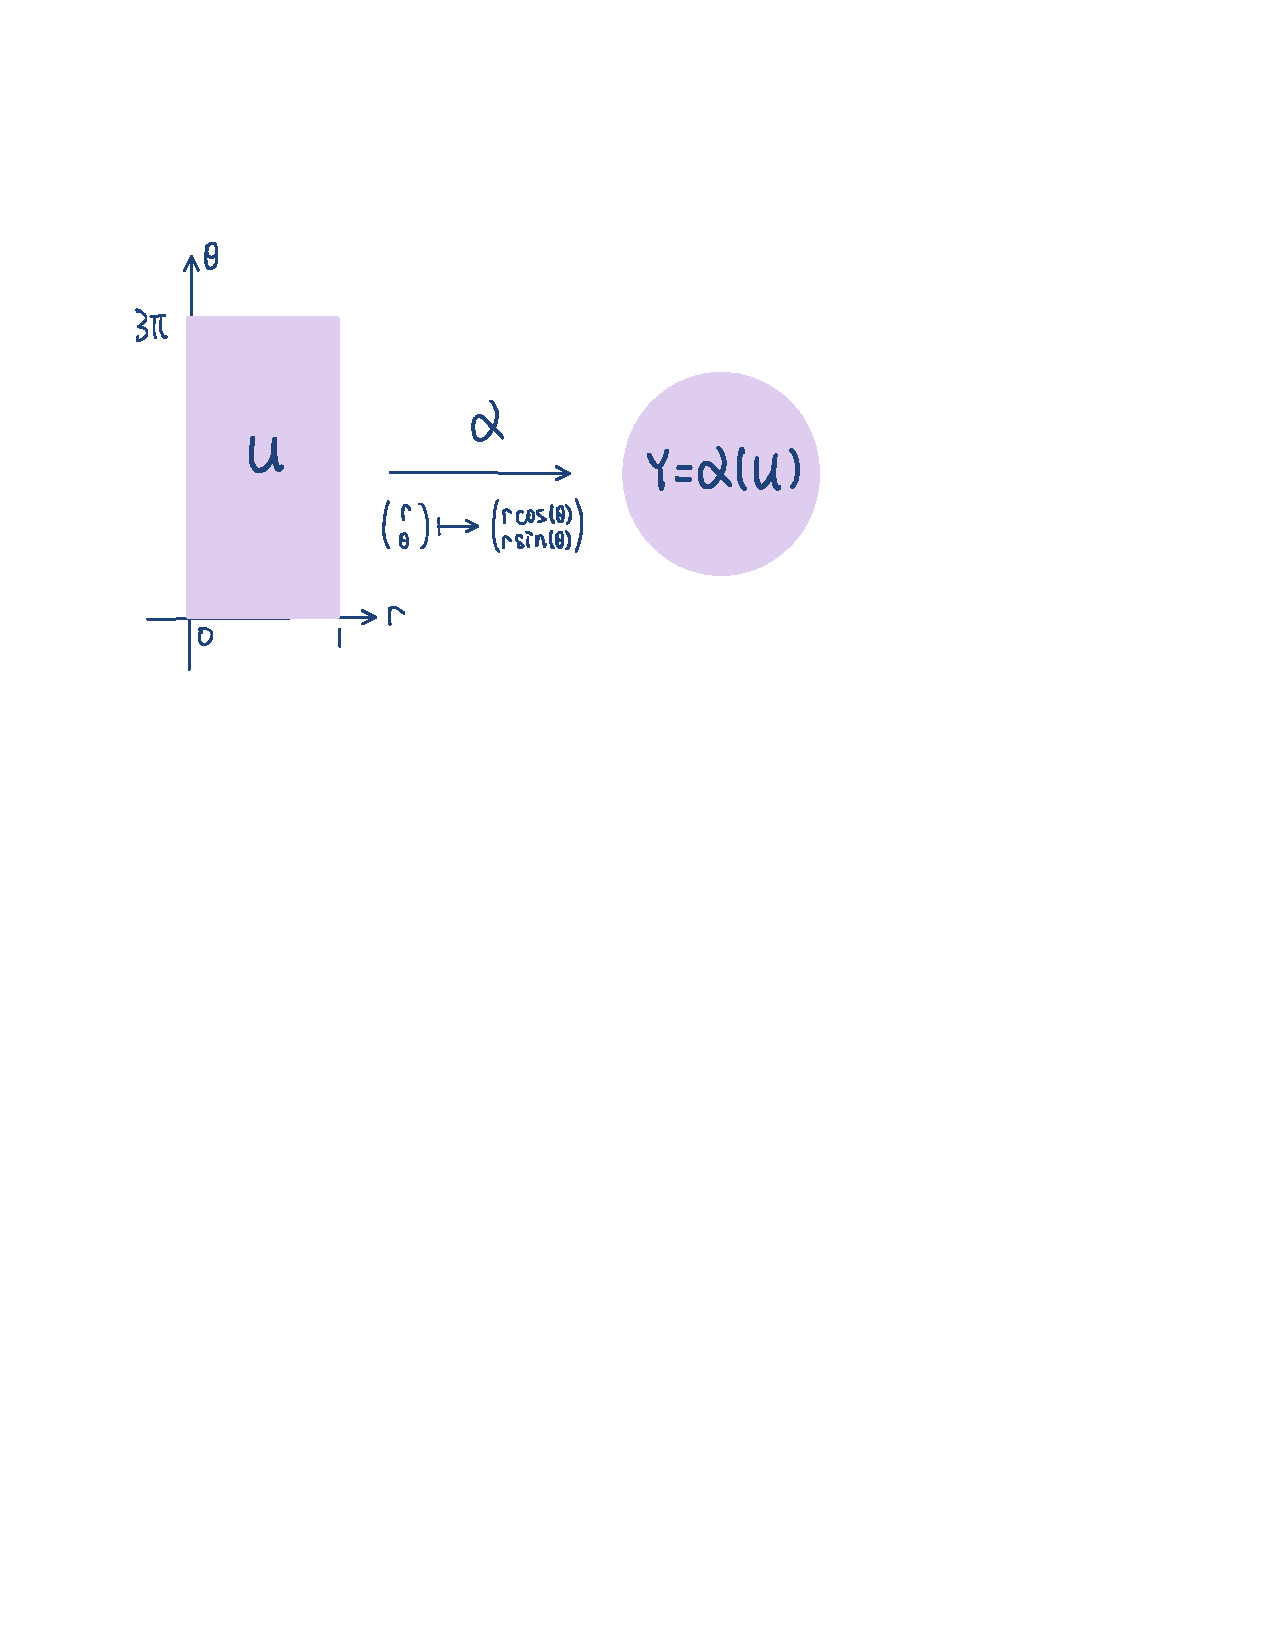
\includegraphics[scale=0.8]{par-manifold.pdf}
\end{center}
Here we have: $V_2(Y_\alpha) = \int_U r = \int_0^1 \int_0^{3\pi} r\, d\theta \, dr = \frac{3}{2}\pi$.\\

\note Let $U$ and $V$ be open sets, $\alpha \in C^r(U,\R^n)$, $\beta\in C^r(V,\R^n)$ with $\alpha(U) = \beta(V)$. \\
If there is a diffeomorphism $g$ from $U$ to $V$, then we can write:
\begin{align*}
V_k(Y_\alpha) &= \int_U \sqrt{\det((D(\beta\circ g))^TD(\beta \circ g))} \\
&= \int_U \sqrt{\det\left((Dg)^T \, \left((D\beta)^T\circ g\right) \, \left(D\beta)\circ g\right)\, Dg\right)}\\
&= \int_U \sqrt{\det(Dg^T) \cdot \det(((D\beta)^T\circ g)(D\beta\circ g))\cdot \det (Dg)}\\
&= \int_U \sqrt{\det(((D\beta)^T\circ g)(D\beta\circ g))} |\det(Dg)|\\
&= \int_V \sqrt{\det((D\beta)^T(D\beta)}\\
&= \int_V \mathcal{V}(D\beta)\\
&= V_k(Y_\beta)
\end{align*}

\begin{defn}
Let $Y_\alpha$ be a parametrized $k$-manifold of class $C^r$ with $Y = \alpha(U)$. Given $f \in C(Y,\R)$, we define: $$\int_{Y_\alpha} f\, dV \coloneqq ext \int_U (f\circ \alpha) \mathcal{V}(D\alpha)$$
\end{defn}
\hfill\break
\exercise Let $U$ and $V$ be open sets, $\alpha \in C^r(U,\R^n)$, $\beta\in C^r(V,\R^n)$ with $\alpha(U) = \beta(V)$. If there is a diffeomorphism $g$ from $U$ to $V$, we have $\int_{Y_\alpha} f\, dV = \int_{Y_\beta} f \, dV$ for $f \in C(Y,\R)$. \\

\note Let $Y_\alpha$ be a parametrized $k$-manifold of class $C^r$, let $h:Y \to Z \ \ \ \vec{z}\mapsto B\vec{z}+\vec{h}$ be an isometry with orthogonal matrix $B$ and $Z = h(Y)$, and let $f:Z \to \R$ be a continuous function. Here $Z_{h\circ \alpha}$ defines a parametrized $k$-manifold, we can write the following:
\begin{align*}
\int_{Z_{h\circ \alpha}}f\, dV = \int_U (f\circ h \circ \alpha) V(B \cdot D\alpha) = \int_U(f\circ h\circ \alpha) V(D\alpha) = \int_{Y_\alpha} (f\circ h) \, dV
\end{align*}
Consider $\delta:Y \to M \ \ \ \vec{x}\mapsto r\vec{x}$ for some $r \in \R$ with $M = \delta(Y)$. $M_{\delta \circ \alpha}$ defines a parametrized $k$-manifold, let $f:M \to \R$ be a continuous function, we can write the following:
\begin{align*}
\int_{M_{\delta\circ \alpha}}f\, dV =r^k \int_{Y_\alpha} f\circ \delta\, dV
\end{align*}

\example 
\begin{center}
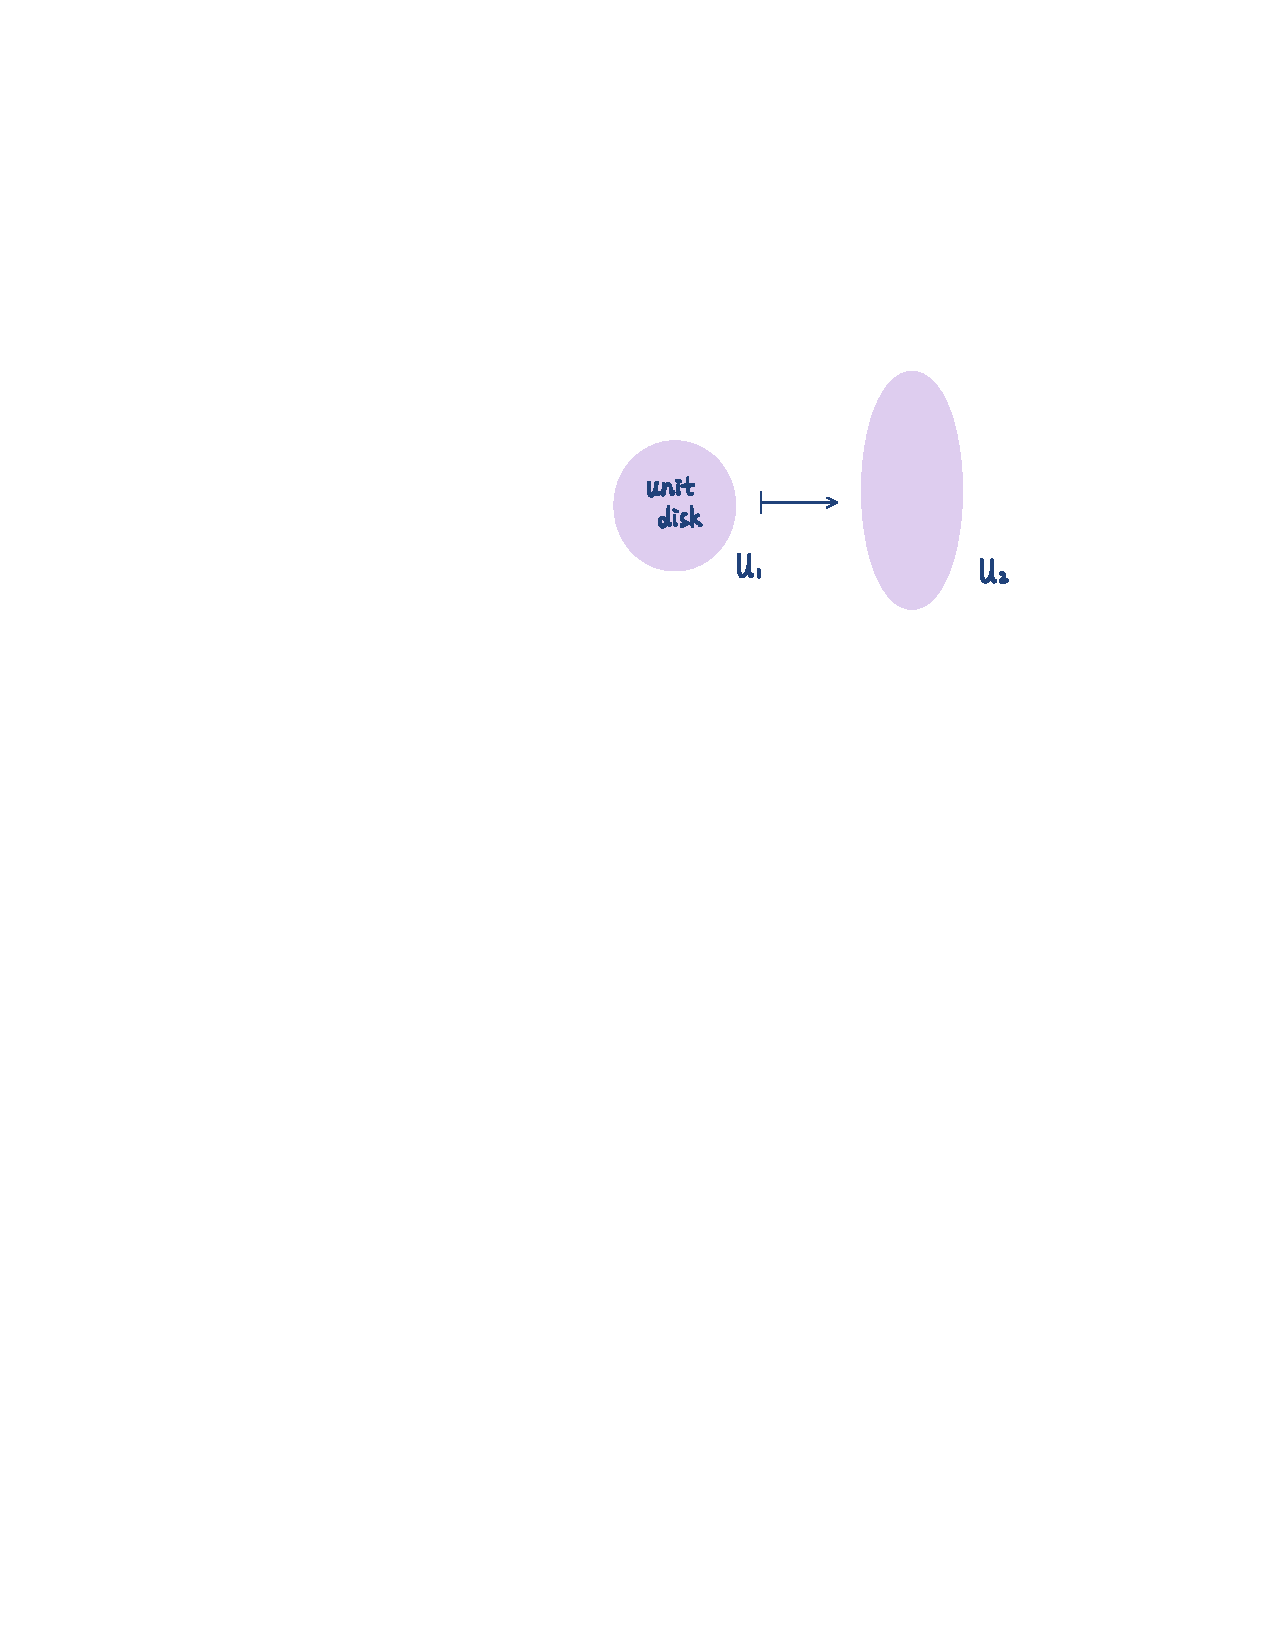
\includegraphics[scale=0.8]{manifold-disk.pdf}
\end{center}
$U_2$ is the image of the function $\alpha:U_1 \to U_2 \ \ \ (x,y) \mapsto (x,2y)$. Here we can write:
$$V_2(U_2)= 2V_2(U_1) \qquad \qquad \qquad \qquad V_1(Bd(U_1)) = 2\pi$$
\hfill\break



\newpage
\section[Manifolds without Boundaries]{\color{red}Manifolds without Boundaries\color{black}}
\begin{defn}
Given $r,k,n \in \N$, a set $M \subseteq \R^n$ is called a k-manifold without boundary of class $C^r$ provided that for all $\vec{p} \in M$, there exist a set $V \subseteq M$ that contains $\vec{p}$, a set $U\subseteq \R^k$, with $V$ being open in $M$ and $U$ being open in $\R^k$, and a homeomorphism $\alpha \in C^r(U,V)$, with $rank(D\alpha(\vec{x})) = k$ for all $\vec{x}\in U$. The map $\alpha$ is called a coordinate patch on $M$ about $\vec{p}$.
\end{defn}

\example Consider the set $M = \{(x,y) \mid x^2 = y^3\}$, and the map $\alpha:\R \to M \ \ \ t \mapsto (t^3,t^2)$, here $\alpha $ is a homeomorphism, but $\alpha'(0) = 0$, so we have $rank(\alpha'(0)) = 0$. With such $\alpha$, $M$ is not a $1$-manifold, but $M \setminus \{(0,0)\}$ is a $1$-manifold. \\

\example Consider the set $M = \{(x,y) \mid y=|x| \}$, and the map $\alpha:\R \to M \ \ \ t\mapsto (t^3, |t|^3)$, here $\alpha$ is a homeomorphism, but $\alpha'(0) = 0$, so we have $rank(\alpha'(0)) = 0$. With such $\alpha$, $M$ is not a $1$-manifold. \\

\example Consider the set $M = \{(x,y) \mid y = x^2\}$. The map $\alpha:\R \to M \ \ \ t\mapsto (t^3,t^6)$ defines a homeomorphism, but $\alpha'(0) = 0$. The map $\widetilde{\alpha}:\R \to M \ \ \ t\mapsto (t,t^2)$ also defines a homeomorphism, and we have $\widetilde{\alpha}'(x) \neq 0$ for all $x \in \R$, here we found $\widetilde{\alpha}$ that satisfies the conditions that makes $M$ a $1$-manifold, and $\widetilde{\alpha}$ is called a coordinate patch on $M$\\

\example Check Section 23 Example 3 on Munkres Page 198.\\

\example Consider the set $M = \{(x,y) \mid x^2+y^2 = 1\}$. Note that continuous functions map compact set to compact set, here $M$ is compact, hence we cannot handle $M$ with a single coordinate patch, but we can make $M$ a $1$-manifold without boundary using the following four coordinate patches to cover all points on $M$:
$$\alpha_1: (-1,1) \to M \ \ \  x\mapsto \left(x,\sqrt{1-x^2}\right) \qquad\qquad\qquad\alpha_2: (-1,1) \to M \ \ \  y\mapsto \left(\sqrt{1-y^2},y\right) $$
$$\alpha_3: (-1,1) \to M \ \ \  y\mapsto \left(-\sqrt{1-y^2},y\right)\qquad\qquad\qquad\alpha_4: (-1,1) \to M \ \ \  x\mapsto \left(x,-\sqrt{1-x^2}\right)$$

\example Consider the set $M=\{ \vec{x}\in \R^n \mid ||\vec{x}||=1\}$. One might use the following $2n$ coordinate patches to make $M$ a $n-1$-manifold:
\begin{align*}
&\alpha_1: \R^{n-1} \to \R^n \ \ \ (x_1,x_2,\cdots, x_{n-1})\mapsto \left(x_1,x_2,\cdots, x_{n-1}, \sqrt{1-\sum_{i=1}^{n-1} x_i^2}\right)\\
&\alpha_2: \R^{n-1} \to \R^n \ \ \ (x_1,x_2,\cdots, x_{n-1})\mapsto \left(x_1,x_2,\cdots, x_{n-1}, -\sqrt{1-\sum_{i=1}^{n-1} x_i^2}\right)\\
&\alpha_3: \R^{n-1} \to \R^n \ \ \ (x_1,x_2,\cdots, x_{n-1})\mapsto \left(x_1,x_2,\cdots, x_{n-2}, \sqrt{1-\sum_{i=1}^{n-1} x_i^2}\ , x_{n-1}\right)\\
&\alpha_4: \R^{n-1} \to \R^n \ \ \ (x_1,x_2,\cdots, x_{n-1})\mapsto \left(x_1,x_2,\cdots,x_{n-2}, -\sqrt{1-\sum_{i=1}^{n-1} x_i^2}\ ,x_{n-1}\right)\\
&{}\qquad\qquad\qquad\qquad\qquad\qquad\qquad\vdots\\
&\alpha_{2n-1}: \R^{n-1} \to \R^n \ \ \ (x_1,x_2,\cdots, x_{n-1})\mapsto \left(\sqrt{1-\sum_{i=1}^{n-1} x_i^2}\ ,x_1,x_2,\cdots, x_{n-1}\right)\\
&\alpha_{2n}: \R^{n-1} \to \R^n \ \ \ (x_1,x_2,\cdots, x_{n-1})\mapsto \left(-\sqrt{1-\sum_{i=1}^{n-1} x_i^2}\ ,x_1,x_2,\cdots, x_{n-1}\right)\\
\end{align*}
\newpage

Let $M$ be a manifold. For $p\in M$, there might be two coordinate patches for $p$, $\alpha_1:U_1\to V_1$ and $\alpha_2:U_2\to V_2$, such that $\alpha_1(q_1) = p$ and $\alpha_2(q_2) = p$. 
\begin{center}
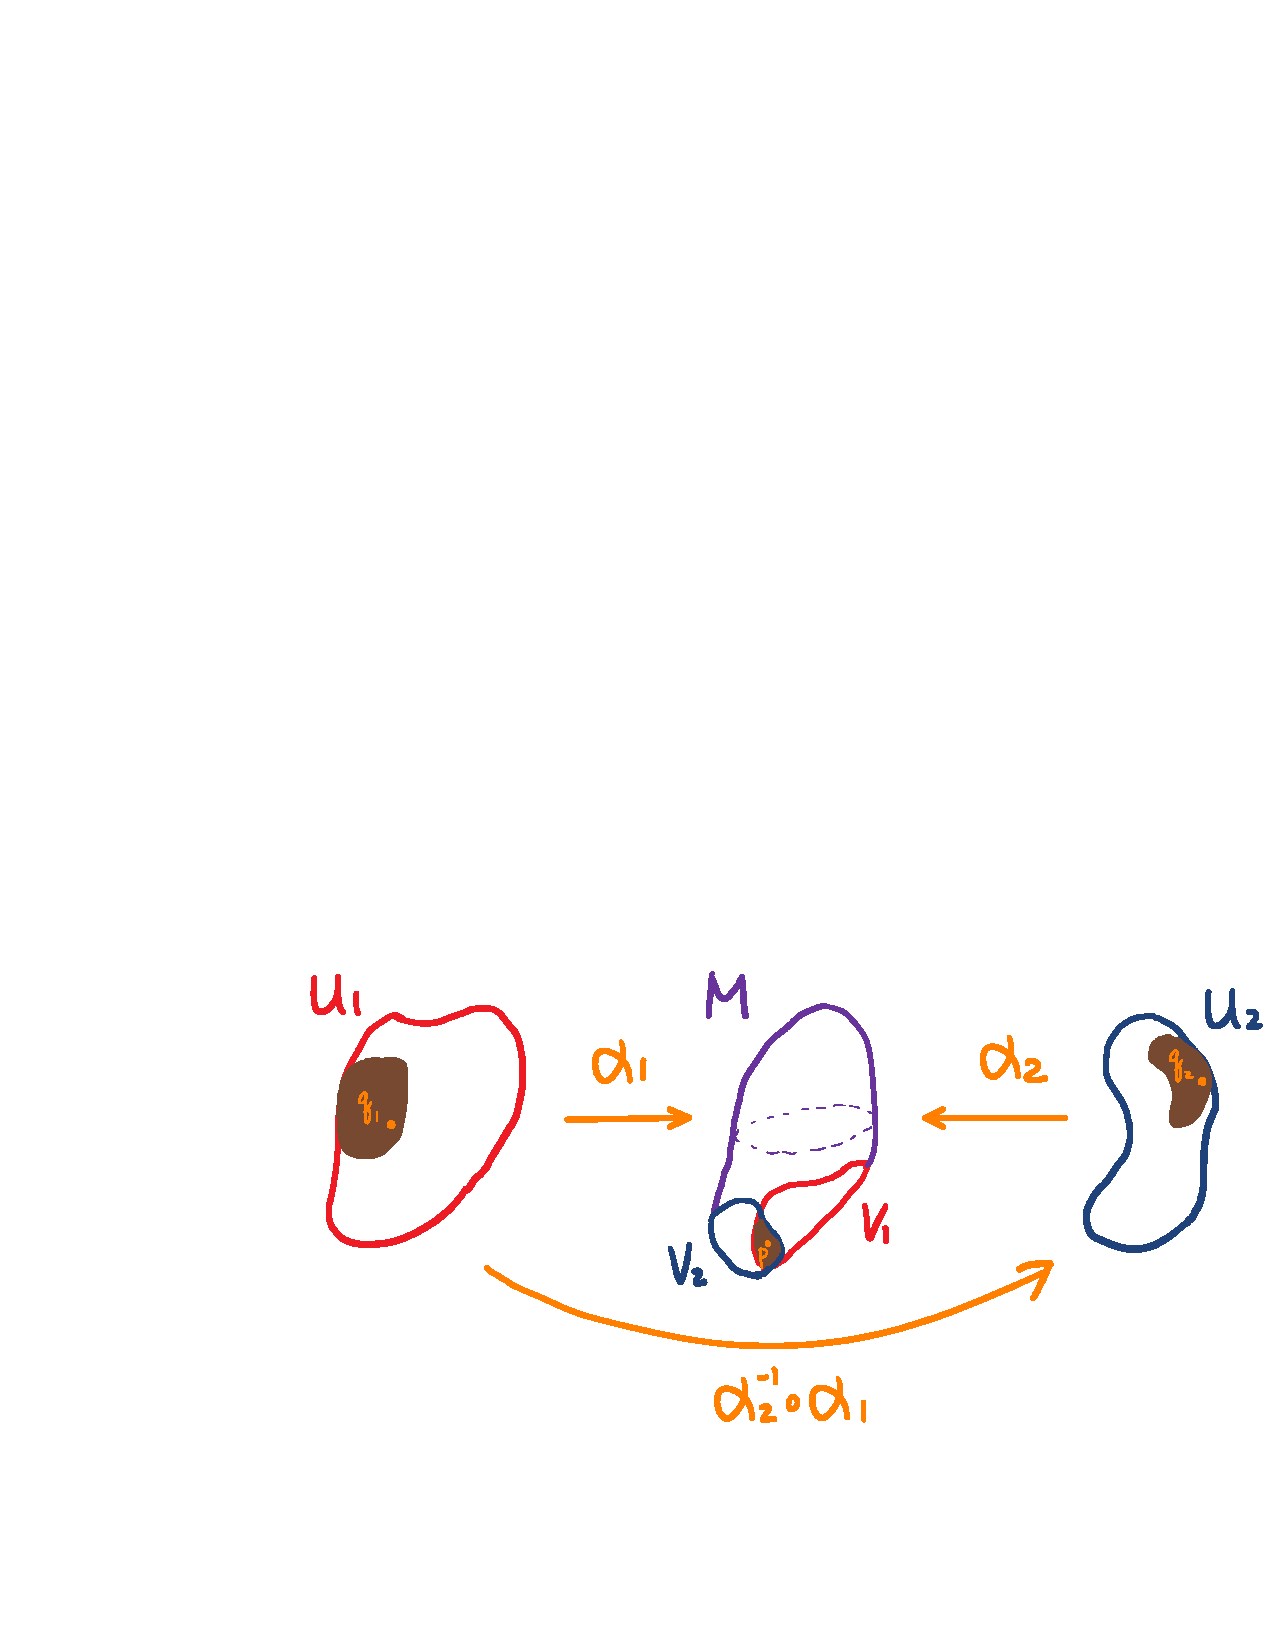
\includegraphics[scale=0.69]{coorPatch.pdf}
\end{center}
Here we note that $\alpha_2^{-1}\circ \alpha_1$ is of $C^r$ type when defined, and $(\alpha_2^{-1}\circ \alpha_1)^{-1} = \alpha_1^{-1} \circ \alpha_2$ is also of $C^r$ type. Hence we know that $\alpha_2^{-1}\circ \approx_1$ is a $C^r$-diffeomorphism. \\

\begin{thm}
For $M \subseteq  \R^n$, the followings are equivalent:
\begin{enumerate}[topsep=3pt,itemsep=-1ex,partopsep=1ex,parsep=1ex]
\item For all $\vec{p}\in M$, there exist a set $U\subseteq \R^k$ open in $\R^k$, a set $V \subseteq M$ open in \mbox{$M$ that contains $\vec{p}$,} and a homeomorphism $\alpha \in C^r(U,V)$ with rank $D\alpha(\vec{x}) = k$ for all $\vec{x}\in U$.  
\item For all $\vec{p}\in M$, there exist a set $A \subseteq \R^k$ open in $\R^k$, a set $V\subseteq M$ open in $M$ that \mbox{contains $\vec{p}$,} a function $g\in C^r(A,\R^{n-k})$, and a coordinate permutation $\rho:\R^n \to \R^n$, such that we have $\rho(V) = Graph(g)$.  
\end{enumerate}
\end{thm}
\begin{proof}
First we will show that (2) implies (1). Take $\alpha: A \to V \ \ \ \vec{x} \mapsto \rho^{-1}(\vec{x},g(\vec{x}))$. We see that $\alpha^{-1} = (\text{projection onto }\R^k)\circ \rho$ is a continuous function. This completes the proof for this direction. Now we will show that (1) implies (2). For $1 \leq s_1 < s_2 <\cdots, < s_k \leq n$ where $s_i \in \N$ for all $1\leq i\leq k$, let $\mathbb{S} = \{s_1,\cdots, s_k\}$. Define $P_\mathbb{S}:\R^n \to \R^k \ \ \ \vec{x}=(x_1,x_2,\cdots,x_n)\mapsto(x_{s_1},x_{s_2},\cdots,x_{s_k})$. Let $\vec{q}\coloneqq \alpha^{-1}(\vec{p})$. Here we can write $D(P_\mathbb{S}\circ \alpha)(\vec{q})= (DP_\mathbb{S}(\vec{p})) \cdot D\alpha(\vec{q}) = P_\mathbb{S}D\alpha(\vec{q}) = (k \text{ selected row of }D\alpha(\vec{q}))$. Hence we can choose $P_\mathbb{S}$ such that $D(P_\mathbb{S}\circ \alpha)$ is invertible. Let $\Omega$ denote the image of $P_\mathbb{S}$. By the Inverse Function Theorem, we can shrink $U,V, \Omega$ to $\widetilde{U},\widetilde{V},\widetilde{\Omega}$ such that $P_\mathbb{S}\circ \alpha$ is a diffeomorphism from $\widetilde{U}$ to $\widetilde{\Omega}$. Let $h = \alpha\circ (P_\mathbb{S}\circ \alpha)^{-1}$, note here we have $P_\mathbb{S}\circ h = P_\mathbb{S}\circ \alpha\circ (P_\mathbb{S}\circ \alpha)^{-1} = $ identity transformation. Let $\rho$ takes $\mathbb{S}$ to $\{1,\cdots, k\}$, one can check $\rho(\widetilde{V}) = Graph(h)$. This completes the proof.
\begin{center}
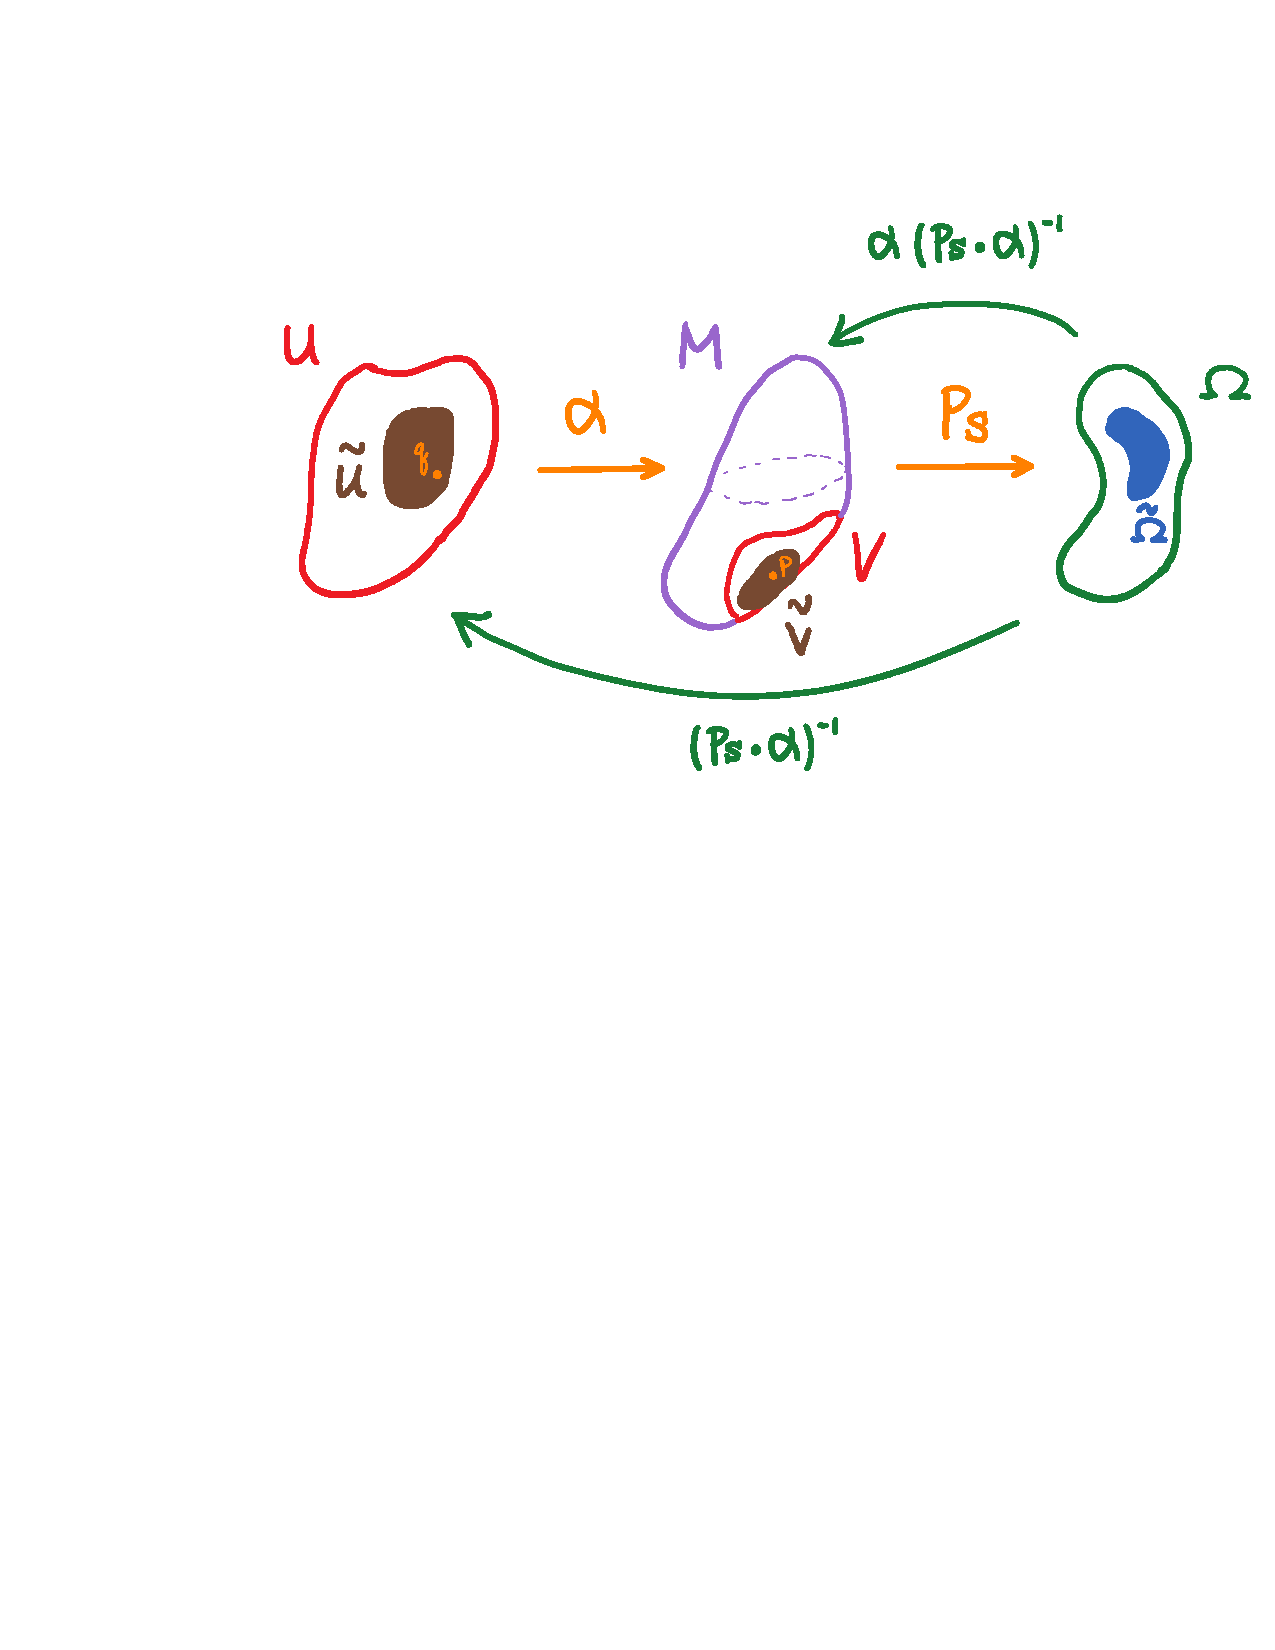
\includegraphics[scale=0.69]{manifoldsDefn.pdf}
\end{center}
\remark $(P_\mathbb{S} \circ \alpha)^{-1} \circ P_\mathbb{S} \in C^r(\rho^{-1}(\widetilde{\Omega}\times \R^{n-k} ),\widetilde{U})$.
\end{proof} 
 
In the settings of Theorem 16.1, a region of $M$ can be viewed as an affine set after a  dilation $\T_{\vec{p}}$ of the region of $M$ centered at $\vec{p}$, we denote this affine set by $\vec{p} + \T_{\vec{p}}(M)$, which is called the tangent space of $M$ at $\vec{p}$. For $\vec{x}$ near $\vec{q}$, we have:
$$\alpha(\vec{x}) \approx \alpha(\vec{q}) + D\alpha(\vec{q}) \cdot (\vec{x}-\vec{q})$$
We observe that $\T_{\vec{p}}(M)$ is approximately $D\alpha(\vec{q}) (\R^k)$. Now we suppose there is another coordinate patch $\that{\alpha}$ for $\vec{p}\in M$, with $\that{\alpha}(\vec{q}') = \vec{p}$. By Chain Rule, we can write:
$$D\that{\alpha}(\vec{q}')(\R^k) = (D\that{\alpha}(\vec{q}'))(D(\that{\alpha}^{-1}\circ \alpha )(\vec{q}))(\R^k) = D\alpha(\vec{q})(\R^k)$$

\begin{thm}
Let $U$ be an open subset of $\R^n$, let $F \in C^r(U,\R^{n-k})$, let $M = F^{-1}(\vec{0})$. If $rank(DF(\vec{x})) = n-k$ for all $\vec{x}\in M$. Then $M$ is a $k$-manifolds without boundary of class $C^r$.
\end{thm}
\begin{proof}
One can apply the Implicit Function Theorem, and show that $M$ is locally a coordinate-permuted $C^r$ graph. Theorem 24.4 on Munkres provides a very similar proof.
\end{proof}

\note The converse of Theorem 16.2 might fail.\\
\note In the settings of Theorem 16.2 and Theorem 16.1, we have $F(\alpha(\vec{q})) = 0$ for all $\vec{q}$ in the domain of $\alpha$, hence by Chain Rule, we can write the following:
$$D(F\circ \alpha)(\vec{q}) = DF(\vec{p})\cdot D\alpha(\vec{q}) = 0 \qquad \Rightarrow \qquad \T_{\vec{p}}(M) = D\alpha(\vec{q})(\R^k) \subseteq \ker (DF(\vec{p}))$$
Here $D\alpha(\vec{q})(\R^k) $ has dimension $k$, and $\ker (DF(\vec{p}))$ has dimension $n-(n-k)= k$, so we have: 
$$\T_{\vec{p}}(M) = \ker (DF(\vec{p}))$$


\exercise $F:\R^n \to \R \ \ \ \vec{x}\mapsto ||\vec{x}||^2 -1$. $F^{-1}(\vec{0})\coloneqq S^{n-1}$.\\
Here we have $DF(\vec{p}) = 2\cdot \vec{p}^T\Rightarrow \ker(DF(\vec{p})) = \{\vec{p}\}^\perp= \T_{\vec{p}}(S^{n-1})$.\\



\remark Let $U$ be an open subset of $\R^{n+k}$, let $f\in C^1(U,\R^n)$ and $h \in C^1(U,\R)$, with $Df = n$. Each $f^{-1}(\vec{a})$ is a $k$-manifold without boundary by Theorem 16.2. Say we want to maximize, or minimize, $h$ under the constraint $f^{-1}(\vec{a})$. Lagrange Multiplier Theorem states that,if $h$ is maximized, or minimized at $\vec{x}$, we must have: $$f(\vec{x}) = \vec{a} \qquad\text{ with }\qquad Dh(\vec{x}) =\vec{\lambda}\cdot Df(\vec{x})$$ 
with some row vector $\vec{\lambda}$. If we vary $\vec{a}$, one might view the pair $(\vec{x},\vec{\lambda})$ as a function of $\vec{a}$ locally via Implicit Function Theorem. In the case where $n=1$, $\vec{a}\in \R$, here we denote $\vec{a}$ as scalar $a$, by argument above, $\vec{x}$ and $\lambda$ are functions of $a$. Here we have $f(\vec{x}(a)) = a$, with the following holds:
$$\frac{d}{da}h(\vec{x}(a)) = Dh(\vec{x}(a) ) \cdot \vec{x}'(a) = \lambda(a) Df(\vec{x}(a))\cdot \vec{x}'(a) = \lambda(a) \cdot \frac{d}{da}(f(\vec{x}(a))) = \lambda(a)$$

\newpage
\section[Manifolds which might have Boundaries]{\color{red}Manifold which might have Boundaries\color{black}}
\begin{defn}
For $S \subseteq \R^k$, $g:S \to \R^n$. For some $r \in \N$. $g$ is of $C^r$ type provided that there exists open subset of $\R^k$ that contains $S$, and $G \in C^r(U,\R^n)$ such that $G|_S = g$. If such $G$ exists, then $G$ extends $g$, and we write $g\in C^r(S,\R^n)$.
\end{defn}
\note Let $S\subseteq \R^k$, for $g\in C^r(S,\R^n)$, the extension $G$ of $g$ is not unique in general. For $|\alpha| \leq r$, we have $D^\alpha g \coloneqq D^\alpha G$ on $Int(S)$ and on $\overline{Int(S)}\cap S$. Suppose we have $g(S) \subseteq T \subseteq \R^n$, and let $h\in C^r(T,\R^m)$. We have $h\circ g \in C^r(S,\R^m)$. The extension $G$ of $g$ can be obtained through Whitney Extension Theorem, or, sometimes, simply by using the Taylor Polynomial. \\


\begin{defn}
$$\mathbb{H}_k\coloneqq \{(x_1,x_2,\cdots,x_k)\in \R^k \mid x_k \geq 0\} \qquad\qquad\qquad \mathbb{H}_+^k \coloneqq \{(x_1,x_2,\cdots,x_k)\in \R^k \mid x_k > 0\}$$
\end{defn}
\hfill\break
\begin{defn}
Given $r,k,n \in \N$, a set $M \subseteq \R^n$ is called a $k$-manifold of class $C^r$ provided that, for all $\vec{p}\in M$, there exist a subset $U$ of $\R^k$ open in either $\R^k$ or $\mathbb{H}^k$, a subset $V$ of $M$ open in $M$, and a homeomorphism $\alpha \in C^r(U,V)$ with $rank(D\alpha(\vec{x})) = k$ for all $\vec{x}\in U$. If such $\alpha$ exists for $\vec{p}\in M$, then $\alpha$ is called the coordinate patch on $M$ about $\vec{p}$, and $M$ is also called a $C^r$ manifold which might have  boundary. 
\end{defn}

\note Let $M$ be a $C^r$ manifold which might have  boundary, for $\vec{p}\in M$, let $\alpha_1$ and $\alpha_2$ be coordinate patches on $M$ about $\vec{p}$. Then $\alpha_1^{-1}$ is a $C^r$ function. $\alpha_2^{-1}\circ \alpha_1$ is a $C^r$ diffeomorphism between the domain of $\alpha_2^{-1} \circ \alpha_1$ and domain of $\alpha_1^{-1} \circ \alpha_2$. \\

Let $U$ and $W$ be relatively open in $\mathbb{H}_k$, let $\gamma:U \to W$ be a diffeomorphism.\\ 
Then $U \cap \mathbb{H}_+^k$ is open in $\R^k$. $D\gamma(\vec{x})$ is invertible for all $\vec{x}\in U\cap \mathbb{H}_+^k$. By the Inverse Function Theorem, $\gamma(U\cap \mathbb{H}_+^k)$ is open in $\mathbb{H}^k$ and must be contained in $\mathbb{H}_+^k$. Here we have $\gamma(U\cap \mathbb{H}_+^k) \subseteq (W \cap \mathbb{H}_+^k)$. With similar argument applying to $\gamma^{-1}$, we get $\gamma(U \cap \mathbb{H}_+^k) = W \cap \mathbb{H}_+^k$, so we have $\gamma(U\cap (\R^{k-1} \times \{0\}) = W\cap (\R^{k-1} \times \{0\})$. 


\begin{defn}
Let $M$ be a $k$-manifold. For $\vec{p}\in M$, $\vec{p}$ is called a boundary point of $M$ provided that there exists a coordinate patch $\alpha:U \to V$ on $M$ about $\vec{p}$ such that $U$ is open in $\mathbb{H}^k$, $V$ is open in $M$, and $\vec{p} = \alpha((x_1,x_2,\cdots, x_{k-1},0))$. The set of boundary points of $M$ is called the manifold boundary of $M$. denoted as $\partial M$. For $\vec{q}\in M\setminus \partial M$, $\vec{q}$ is called an interior point of $M$. 
\end{defn}

\begin{lem}
Let $M$ be a $k$-manifold in $\R^n$, and let $\alpha:U \to V$ be a coordinate patch about the point $\vec{p}\in M$. \\If $U$ is open in $\mathbb{H}_k$ and $\vec{p} = \alpha(\vec{x})$ for some $\vec{x}\in \mathbb{H}_+^k$, then $\vec{p}$ is an interior point of $M$.
\\If $U$ is open in $\R^k$, then $\vec{p}$ is an interior point of $M$. 
\end{lem}


\begin{thm}[Theorem 24.4 on Munkres]
Let $M$ be a $k$-manifold, $\partial M$ is a $C^r$ $(k-1)$-manifold without boundary.
\end{thm}
\begin{proof}
For coordinate patch $\alpha:U \to V$ where $V \subseteq M$, it induces coordinate patch defined by: 
\begin{align*}
\hat{\alpha}: \{(x_1,x_2,\cdots, x_{k-1})\mid (x_1,x_2,\cdots, x_{k-1},0) \in U\}&\to \partial M \\ (x_1,x_2,\cdots, x_{k-1})&\mapsto \alpha(x_1,x_2,\cdots, x_{k-1},0)
\end{align*}
\end{proof}

\exercise For $k$-manifold $M_1$ and $M_2$ in $\R^n$. If there exists a diffeomorphism $\alpha:M_1 \to M_2$, then $\alpha|_{\partial M_1}$ is a diffeomorphism from $\partial M_1$ to $\partial M_2$.\\

\example Let $M$ be a $k$-manifold in $\R^n$. Consider the extreme case where we have $k=n$, $n$-manifold without boundary is an open subset of $\R^n$. $n$-manifold which might have boundary is an open subset of $\R^n$ union with a set $\partial M$ that is an $n-1$-manifold without boundary, and $\partial M$ is contained in the topological boundary of $M$. \\

\example
Consider a closed triangle in $\R^2$, which is not a $2$-manifold, because the boundary of the closed triangle fails to be a 1-manifold. If we take out the vertices of the closed triangle, that becomes a $2$-manifold. If we take out all boundary points of the closed triangle, then we get a 2-manifold without boundary.\\
\newpage
Here we extend the definition for $k$-manifolds in $\R^n$ for the case where $k=0$: \begin{defn} 
A countable collection of of points in $\R^n$ is called a $0$-manifold in $\R^n$.
\end{defn}

\remark $0$-manifold $M$ has $\partial M = \emptyset$. $M$ is a $0$-manifold if and only if each singleton subset of $M$ is relatively open, that is, if and only if each point of $M$ is isolated. \\

\note A set $M$ is a compact $0$-manifold $\iff$ $M$ is a finite set. For such we write $$\int_M fdV \coloneqq \sum_{x \in M} f(x)$$
\note All $0$-manifolds are countable sets. \\

\exercise For open subset $U$ of a $k$-manifold $M$, $U$ is a $k$-manifold.\\

\begin{thm}
Every $k$-manifold $M$ can be decomposed uniquely as a disjoint union of open connected $k$-manifolds, which are called the components of $M$. 
\end{thm}
\begin{proof}
The proof of this theorem can be found on Math 395 Supplement materials Section $H$.
\end{proof}


\begin{thm}
Every connected 1-manifold of class $C^r$ is $C^r$-diffeomorphic to an interval in $\R$ or to the circle $S^1$. 
\end{thm}
\begin{proof}[Outline of the proof]
Suppose $M$ is a connected $1$ manifold. Let $x_0 \in M \setminus \partial M$. One might show:\\

\exercise For any $x_1 \in M\setminus\{ x_0\}$, there is $I \subseteq M$ such that $I$ is homeomorphic to closed interval with $\partial I = \{ x_0,x_1\}$, this can be viewed as a path connecting $x_0$ and $x_1$, one can mimic the proof of Math 395 HW3 Q4 to construct such path.\\

Now consider the following two cases:\\
(1) There exists only one such $I$ connecting $x_0$ and $x_1$ for each $x_1\in M\setminus\{ x_0\}$. Denote such $I$ as $I_{x_0,x_1}$. Consider a partition of $M\setminus \{x_0\}$ into two subsets, one is called the left of $x_0$ and the other one is called the right of $x_0$. $x_1 \in M\setminus \{x_0\}$ belongs to left or right of $x_0$ according to whether $I_{x_0,x_1}$ is contained in the left of $x_0$ union with $\{x_0\}$, or the right of $x_0$ union with $\{x_0\}$, as defined by the following:

\begin{center}
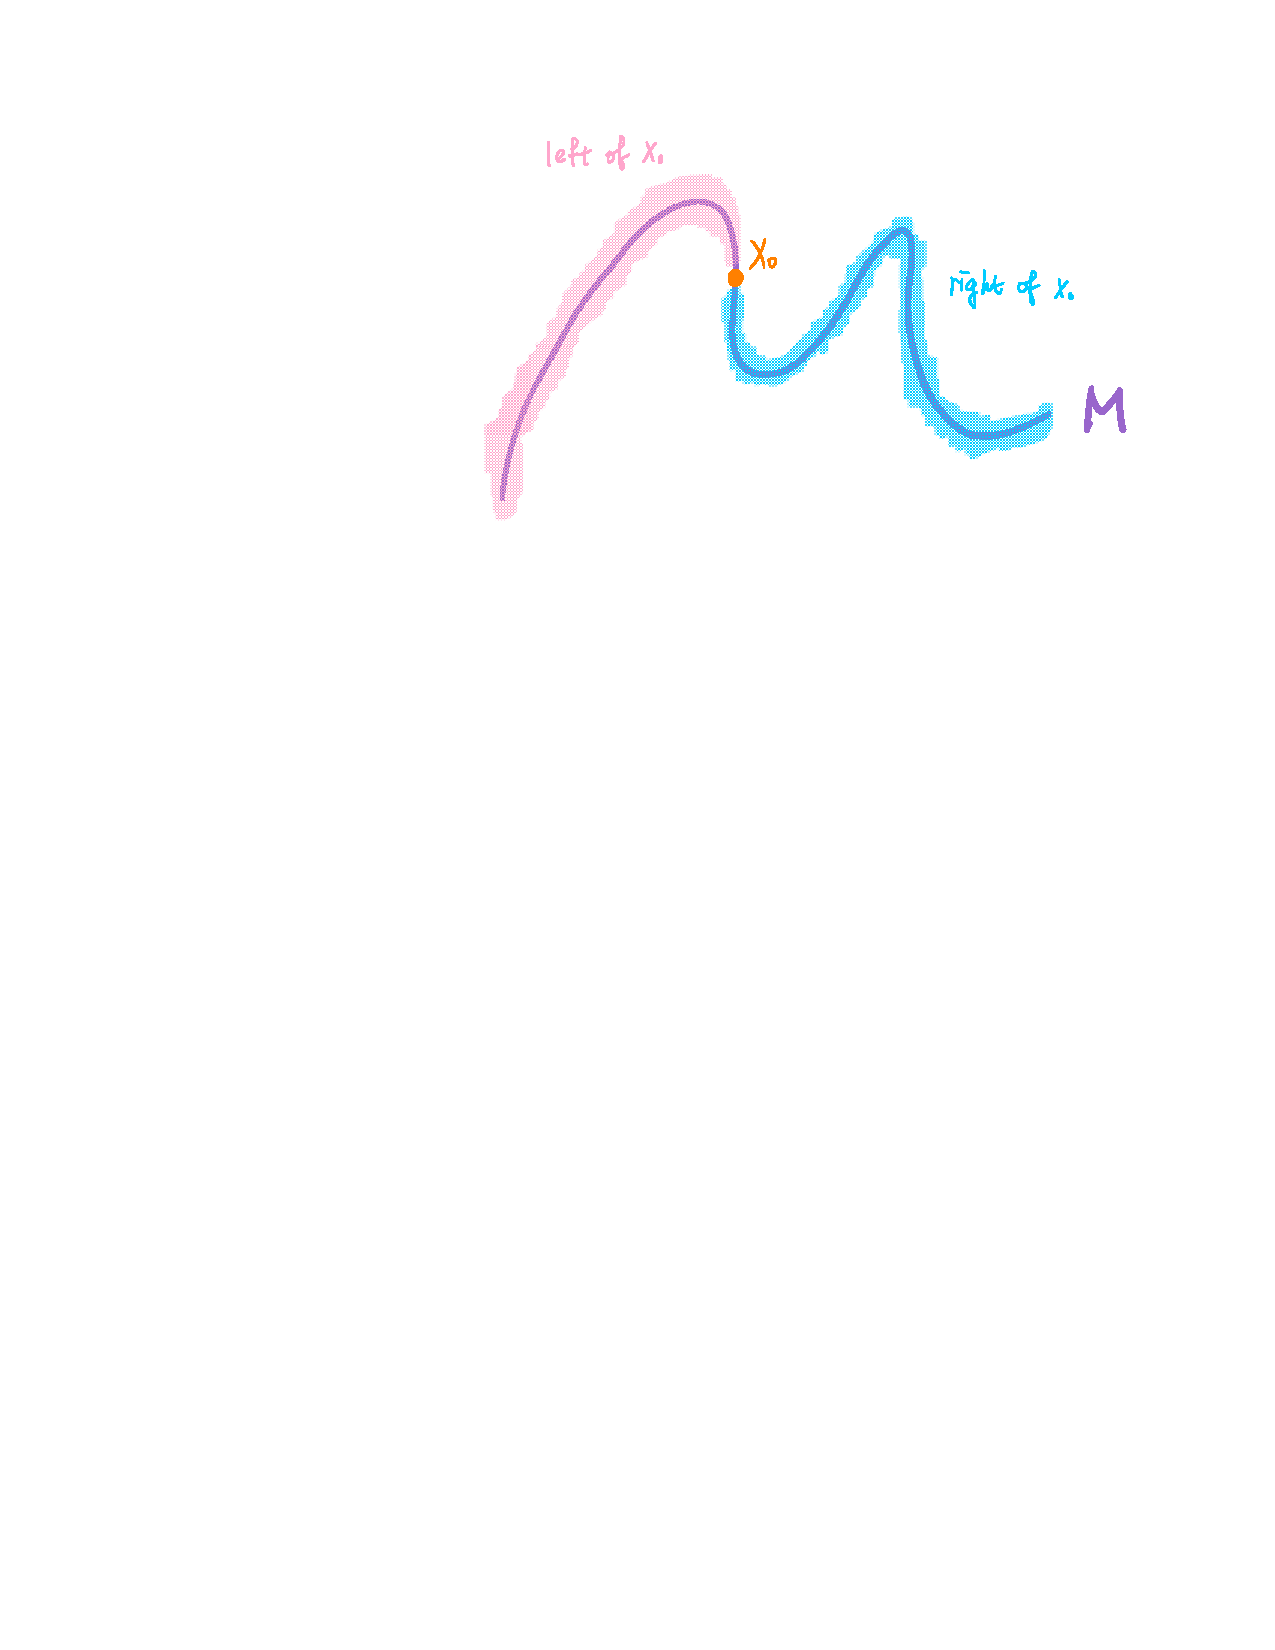
\includegraphics[scale=0.5]{1-manifoldHom.pdf}
\end{center}

Now consider a function $f:M \to \R$ defined by the following: 
$$f:M \to \R \ \ \ x_1\mapsto\begin{cases} 0 & x_1 = x_0 \\ V_1(I_{x_0,x_1}) & x_1\text{ lies on the right of }x_0 \\ -V_1(I_{x_0,x_1}) & x_1\text{ lies on the left of }x_0\end{cases}$$ 
One can check that $f:M \to \R$ is continuous, and here $f(M)$ is connected because $M$ is connected, then we know that $f(M)$ must be an interval. Consider the following exercise:\\

\exercise $\{y \in f(M)\mid \#(f^{-1}(y)) = 1\}$ is open in $f(M)$, closed in $f(M)$, and contains $0$. \\

with this exercise, we know that $f:M \to f(M)$ is a continuous bijection. Consider coordinate patch $\alpha: U \to V \subseteq M$ with $U$ being an interval and $[t_0,t_1] \subseteq U$, we have $f(\alpha(t_2))$ either being greater than or less than $f(\alpha(t_1))$. WLOG, we suppose $f(\alpha(t_2)) > f(\alpha(t_1))$. We can write the following:
$$\int_{[t_1,t_2]} ||D\alpha|| = \int_{[t_1,t_2]} \mathcal{V}(D\alpha) = V_1(\alpha([t_1,t_2])) = f(\alpha(t_2)) - f(\alpha(t_1))$$
Then by the Fundamental Theorem of Calculus, we see that $D(f\circ \alpha) = ||D\alpha||$. From the definition of coordinate patch, we know that $D(f\circ \alpha) = ||D\alpha|| > 0$. Here $D\alpha$ and $||D\alpha||$ are both $C^{r-1}$ functions, note that the norm function is of $C^\infty$ type except at $\vec{0}$, but $D\alpha$ is nonzero. Then we know that $D(f\circ \alpha)$ is of $C^{r-1}$ type and hence $f\circ \alpha$ is of $C^r$ type. Hence $f = (f\circ \alpha) \circ \alpha^{-1}$ is also of $C^r$ type.  Since $D(f\circ \alpha) \neq 0$, then by Inverse Function Theorem, we know that $(f\circ \alpha)^{-1}$ is of $C^r$ type, and hence $f^{-1} = \alpha \circ (f\circ \alpha)^{-1}$ is also of $C^r$ type. This completes the proof for case (1).\\

Now consider case (2), in which case there exists $I_1, I_2 \subseteq M$ that are homeomorphic to closed intervals in $\R^2$ with $\partial I_1 = \{x_0,x_1\} = I_2$ and $I_1 \neq I_2$, for some $\vec{x}_1 \in M\setminus\{x_0\}$. Without lost of generality, here we assume $I_1 \nsubseteq I_2$. We will make use of the following exercises:\\

\exercise $I_1 \setminus I_2$ is relatively open in $I_1 \setminus \partial I_1$, relatively closed in $I_1 \setminus \partial I_1$, and nonempty.\\

From this exercise, we know that $I_1 \setminus I_2 = I_1 \setminus \partial I_1$, hence we have $I_1 \cap I_2 = \{x_0,x_1\}$. \\

\exercise $I_1 \cup I_2$ is relatively open in $M$, relatively closed in $M$, and non-empty.\\

With these exercises, we conclude that $M = I_1\cup I_2$. From similar constructions in case (1), one can obtain the following $C^r$-diffeomorphisms:
\begin{align*}
f_1&:I_1 \to [0, V_1(I_1)] \ \ \ \vec{x}_2\mapsto V_1(I_{x_0,x_2})\\
f_2&:I_2 \to [-V_1(I_2),0] \ \ \ \vec{x}_2\mapsto -V_1(I_{x_0,x_2})
\end{align*}


Let $l_1\coloneqq  V_1(I_1) $ and $l_2 \coloneqq V_1(I_2)$, and consider the following map:
$$\mu:M \to \R^2 \ \ \ \vec{x} \mapsto \begin{cases}\left(\cos\frac{2\pi f_1(\vec{x})}{l_1+l_2}, \sin\frac{2\pi f_1(\vec{x})}{l_1+l_2}\right) & \vec{x}\in I_1\\
\left(\cos\frac{2\pi f_2(\vec{x})}{l_1+l_2}, \sin\frac{2\pi f_2(\vec{x})}{l_1+l_2}\right) & \vec{x}\in I_2\\
\end{cases}$$
One can verify that $\mu$ defines a diffeomorphism from $M$ to $S^1$.
\end{proof}


\begin{corT}
Every connected $1$-manifold is differomorphic to one of the followings:
$$1.\ \ (0,1) \qquad\qquad\qquad
2.\   \ [0,1] \qquad\qquad\qquad
3.\   \ [0,1)\qquad\qquad\qquad
4.\   \ S^1$$
\end{corT}
\begin{proof}
Use the arctangent function and some affine maps. For the uniqueness, we note that diffeomorphism preserves compactness, and also note that if two 1-manifolds are diffeomorphic, then their boundary points of manifolds are also diffeomorphic to each other, hence the manifold boundaries of these two $1$-manifolds have the same cardinality. 
\end{proof}


\begin{thm}
Every compact connected $2$-manifold without boundary in $\R^3$ is diffeomorphic to a sphere in $\R^3$, or a sphere glued with some handles.
\begin{center}
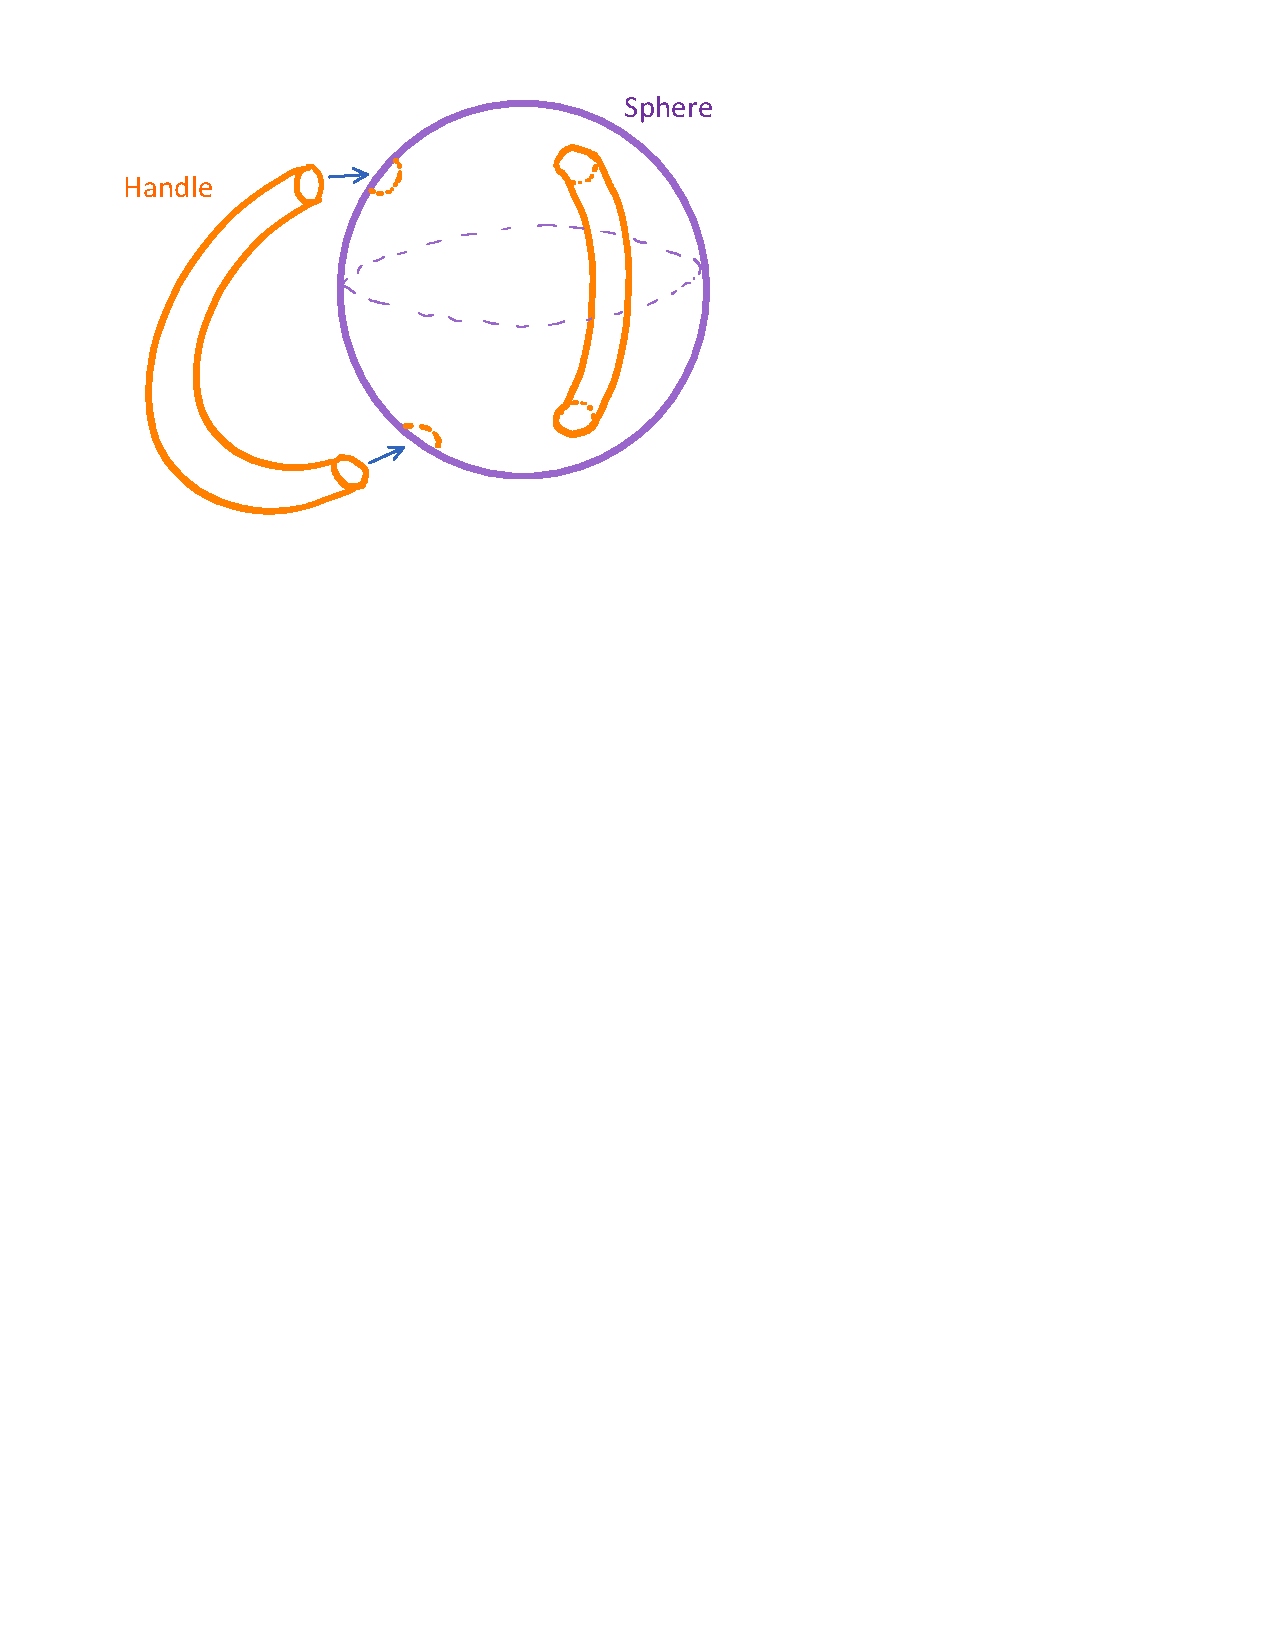
\includegraphics[scale=0.8]{handleBody.pdf}
\end{center}
\end{thm}

If a $2$-manifold with boundary lives in $\R^4$ or higher dimensions, one can glue a disk along the boundary of a Mobius strip to get a projective plane.\\

\begin{thm}
More generally, every compact connected $2$-manifold without boundary in $\R^n$ is diffeomorphic to one of these with handles: (1) a sphere with handles, (2) a projective plane, (3) a Klein bottle.
\end{thm}

One can glue two disks to get a sphere $S^2$ in $\R^3$, glue a disk to boundary of Mobius strip to get a projective plane in $\R^4$, and glue two Mobius strip to get a Klein Bottle in $\R^4$.








\newpage
\section[One-forms and Pullbacks]{\color{red}One-forms and Pullbakcs\color{black}}
\begin{defn}
A $1$-form on an open subset $A$ of $\R^n$ is a continuous function from $A$ to $\R^n_{row}$
\end{defn}

\note Here $R^n_{row}$ is the space of vectors in $\R^n$ represented by row vector. \\

\remark For notation, one might write $(\R^n)^* \coloneqq R^n_{row}$.\\

\example Let $A$ be an open subset of $\R^n$. For $f \in C^1(A,\R)$, the function $Df$ which maps $\vec{x}$ to $Df(\vec{x})$ is a $1$-form. In multivariate differentiation, the operator $D$ takes functions defined on some open subset of $\R^n$ to matrices in $Mat(m,n)$. In the case we $m=1$, we denote the operator $D$ as $d$, which takes functions defined on some open subset of $\R^n$ to $1$-forms.\\

\begin{defn}
Let $A$ be an open subset of $\R^n$, $B$ be an open subset of $\R^m$, let $\alpha \in C^1(B,A)$, and let $\omega$ be an $1$-form defined on $A$.  $\alpha^*\omega \coloneqq (\omega\circ \alpha) \cdot D\alpha$ is called the pullback of $\omega$ by $\alpha$. 
\end{defn}

\remark In the settings of definition 18.0.0.0.2, $\omega\circ \alpha$ is an $1 \times n$ matrix and $D\alpha$ is an $n \times m$ matrix, hence $\alpha^*\omega$ is an $1 \times m$ matrix, which is an $1$-form on $B$.\\

\note For $\R$-valued function $f$ defined on an open subset $A$ of $\R^n$, and $\alpha\in C^1(B,A)$ where $B$ is an open subset of $\R^m$, we can write the following: 
$$\alpha^*df = (df\circ \alpha)\cdot D\alpha =(Df\circ \alpha)\cdot D\alpha = D(f\circ \alpha) = d(f\circ \alpha)$$ 
%Since we have $f\circ \alpha = \alpha^*f$, so $\alpha^*df = d(\alpha^*f)$. \\
\note \textbf{Fundamental Theorem of Calculus II for one-forms}\\
For $C^1$ type function $\alpha:[a,b]=I \to A$ where $A$ is an open subset of $\R^n$, with $\omega$ being an $1$-form on $A$. Then $\alpha^*\omega$ is a $1$-form on $I$, which can be viewed as $\R$-valued function. Consider the $1$-manifold $Y_\alpha$, we can define the following:
$$\int_{Y_\alpha} \omega \coloneqq \int_I \alpha^*\omega$$
For $C^1$ type function $f$ defined on $A$, we can write the following: 
$$\int_{Y_\alpha} df = \int_I \alpha^*df = \int_I d(f\circ \alpha) = \int_I (f\circ \alpha)'= (f\circ \alpha)(b) - (f\circ \alpha) (a) = f(\alpha(b)) - f(\alpha(a))\coloneqq \Delta_{Y_\alpha}f$$
Here we get the results by the Fundamental Theorem of Calculus II. \\


\example Let $A$ be an open subset of $\R^n$. For $f\in C^1(A,\R)$, $df:\vec{x} \to Df(\vec{x})$ is a $1$-form. We write:
\begin{align*}
df &= \bmat{\frac{\partial f}{\partial x_1}&\frac{\partial f}{\partial x_1} &\cdots& \frac{\partial f}{\partial x_n}}\\ &= \frac{\partial f}{\partial x_1}\bmat{1&0&\cdots&0} + \frac{\partial f}{\partial x_2}\bmat{0&1&0&\cdots&0} + \cdots + \frac{\partial f}{\partial x_n}\bmat{0&0&\cdots&1} \\&= \frac{\partial f}{\partial x_1} dx_1 + \frac{\partial f}{\partial x_2 }dx_2 + \cdots + \frac{\partial f}{\partial x_n}dx_n
\end{align*}
Here $dx_i \coloneqq d\pi_i$, where $\pi_i : \R^n \to \R \ \ \ (x_1,x_2,\cdots, x_n)\mapsto x_i$ is the projection function.
In general, for $1$-form defined on $A$, we write $\omega = \bmat{\omega_1 &\omega_2 &\cdots &\omega_n} = \omega_1 dx_1 +\omega_2 dx_2 + \cdots + \omega_n dx_n$.\\

\begin{defn}
Let $f:\R^n \to \R$ be a $C^1$ function, and let $\alpha:\R^m \to \R^n$, we write $\alpha^{*,0}f = f\circ \alpha$.
\end{defn}


\note In the settings of Definition 18.0.0.3, $\alpha^*df = d(\alpha^{*,0}f)$\\
\note Let $\omega$ be a $1$-form defined on open subset $A$ of $\R^n$, let $B$ be an open subset of $\R^m$, let $C$ be open subset of $\R^k$, and let $\alpha_1 \in C^1(B,A)$, and let $\alpha_2 \in C^1(C,B)$, we have $(\alpha_2 \circ \alpha_1)^*\omega = \alpha_1^*(\alpha_2^*\omega)$\\
\newpage
\example Consider the map $\alpha:\R^2 \to \R^2$ defined by $(r,\theta) \mapsto (r\cos(\theta), r\sin(\theta))$. \\We can write the following:
\begin{align*}
\alpha^* \left(\frac{x_1}{x_1^2+x_2^2}dx_1 + \frac{x_2}{x_1^2+x_2^2}dx_2  \right)&=\frac{r\cos(\theta)}{r^2}d(r\cos(\theta)) + \frac{r\sin(\theta)}{r^2}d(r\sin(\theta))\\
&=\frac{r\cos(\theta)}{r^2}(\cos(\theta)dr - r\sin(\theta) d\theta)+ \frac{r\sin(\theta)}{r^2}(\sin(\theta) dr + r\cos(\theta)d\theta)\\
&= \frac{1}{r}dr
\end{align*}
Similarly, we have:
$$\alpha^*  \left(\frac{-x_2}{x_1^2+x_2^2}dx_1 + \frac{x_1}{x_1^2+x_2^2}dx_2  \right)=\frac{r\cos(\theta)}{r^2}d(r\cos(\theta)) + \frac{r\sin(\theta)}{r^2}d(r\sin(\theta)) = d\theta$$


\remark Suppose $\omega:[a,b]\to \R$ is a $1$-form on $[a,b]$. Here we can write the following:
$$\int_{[a,b]} \omega = \int_a^b \omega$$


\note Let $I,J$ be intervals of $\R$ such that $\beta:I\to J$ defines a diffeomorphism. \\
For $\alpha \in C^1(I,\R^n)$, let $\omega$ be a $1$-form defined on $Y_\alpha$, we can write the following:
\begin{align*}
\int_{Y_{\alpha\circ \beta}} \omega &= \int_{J} (\alpha\circ \beta)^* =\int_J \beta^*\alpha^*\omega = \int_J ((\alpha^*\omega) \circ \beta)\cdot D\beta
\end{align*}
Here we see that $D\beta = \det(D\beta)$ because $D\beta$ is a $1\times 1$ matrix. Also note that, since $\beta$ defines a diffeomorphism, then $D\beta(x)\neq 0$ for all $x \in J$, and $D\beta$ is continuous, hence $D\beta$ is a negative, or positive function. Then by the Change of Variable Theorem, we can write the following:
\begin{align*}
\int_{Y_{\alpha\circ \beta}} \omega &= \int_J ((\alpha^*\omega) \circ \beta)\cdot D\beta = \begin{cases}\int_I \alpha^*\omega & D\beta(x) > 0,\ \forall x \in J\\\ -\int_I \alpha^*\omega & D\beta(x) < 0,\ \forall x \in J \end{cases}
\end{align*}
On the other hand, we have:
\begin{align*}
\int_{Y_\alpha} \omega = \int_{I} \alpha^*\omega 
\end{align*}
Combining, we can write the following:
\begin{align*}
\int_{Y_{\alpha\circ \beta}} \omega = \begin{cases}\int_{Y_\alpha} \omega & D\beta(x) > 0,\ \forall x \in J\\\ -\int_{Y_\alpha} \omega & D\beta(x) < 0,\ \forall x \in J \end{cases}
\end{align*}

\note For $1$-form $\omega$ defined on open subset $A$ of $\R^n$, and $\alpha\in C^1([a,b] \to A)$we can write:
\begin{align*}
\int_{Y_\alpha} \omega &= \int_{Y_\alpha} \omega_1dx_1+\omega_2dx_2+\cdots +\omega_n dx_n \\&= \int_{I} (\omega_1\circ \alpha)\cdot  D\alpha_1 + (\omega_2\circ \alpha)\cdot  D\alpha_2
+\cdots + (\omega_2\circ \alpha)\cdot  D\alpha_2
\end{align*}

\example In Physics, a force field can be described by a $1$-form $\omega$ defined on an open subset $A$ of $\R^n$. Let $I\subseteq \R$ be an interval, and let $\alpha\in C^1(I,A)$, then $\alpha$ can be viewed as a path of a particle in the $\R^n$ space. The formula $\int_{Y_\alpha} \omega$ describes the work acted on the particle through the path $Y_\alpha$.\\

\example Consider $\alpha : [0,1]\to \R^n \ \ \ t\mapsto (t,t^n)$.\\ Let $\pi_1:\R^2 \to \R \ \ \ (x,y)\mapsto x$, $\pi_2:\R^2 \to \R \ \ \ (x,y)\mapsto y$ be the projection functions, we can write:
\begin{align*}
\int_{Y_\alpha} \pi_2\, d\pi_1 - \pi_1\, d\pi_2 = \int_0^1 t^n  - n t^{n} = \frac{1-n}{n+1}
\end{align*}

\begin{prop}
Let $f:[a,b]\to \R^n$, the followings are equivalent:
\begin{enumerate}[topsep=3pt,itemsep=-1ex,partopsep=1ex,parsep=1ex]
\item There exists a function $g\in C^k(A,\R^n)$ such that $g(x) = f(x)$ for $x\in [a,b]$, with $A$ being an open subset of $\R$ that contains $[a,b]$.
\item $f \in C([a,b])$, with $f|_{(a,b)} \in C^k((a,b),\R^n)$,  and both $\lim_{t \to a^+} f^{(j)}(t)$ and $\lim_{t \to b^-}f^{(j)}(t)$ exist and are finite for $j\in \N$ with $1\leq j \leq k$.
\end{enumerate}
\end{prop}
\begin{proof}
It is trivial to show that (1) implies (2). For (2) implies (1), one can use the Taylor Polynomials to extend the function $f$. 
\end{proof}

\begin{defn}
For interval $[a,b]\subseteq \R$, a function $f:[a,b] \to \R^n$ is said to be of $C^k$ type provided that there exists a function $g\in C^k(A,\R^n)$ such that $g(x) = f(x)$ for $x\in [a,b]$, with $A$ being an open subset of $\R$ that contains $[a,b]$. In such case, we write $f \in C^k([a,b],\R^n)$. 
\end{defn}

\begin{defn}
For interval $[a,b]\subseteq \R$, a function $f:[a,b] \to \R^n$ is said to be of piecewise $C^k$ type provided that $f$ is continuous on $[a,b]$, and $f|_{[t_{j-1},t_j]} \in C^k([t_{j-1},t_j],\R^n)$ for each $j$, where $\{t_1,t_2,\cdots, t_m\}$ defines a partition on $[a,b]$. In such case, we write $f \in C_{pw}^k([a,b],\R^n)$. 
\end{defn}

\example The function $M:[a,b]\to \R^2$ defined by the following is of piecewise $C^k$ type. 
\begin{center}

\includegraphics[scale=0.5]{M.pdf}
\end{center}

\begin{defn}
Let $[a,b]\subseteq \R$ be an interval, let $\{t_1,t_2,\cdots, t_n\}$ defines a partition of $[a,b]$. For piecewise function $\alpha:[a,b]\to \R^n$ that satisfies $\alpha|_{[t_{j-1},t_j]}$ being continuous on  $[t_{j-1},t_j]$, we denote $\alpha_{(j)} \coloneqq \alpha|_{[t_{j-1},t_j]}$.
\end{defn}

\begin{defn}
For $\alpha \in C_{pw}^k([a,b],\R^n)$, $Y \coloneqq \alpha([a,b])$ is usually denoted as $Y_{\alpha}$, and we write the following:
$$\int_{Y_{\alpha}} \omega = \int_{[a,b]} \alpha^*\omega$$
where $\omega $ is a $1$-form defined on $Y$. Moreover, for function $f$ such that $df$ is a $1$-form defined on $[a,b]$, we write the following:
$$\int_{Y_\alpha} df = \sum_j \int_{Y_{\alpha_{(j)}}}df = \sum_j \Delta_{Y_{\alpha_{(j)}}} f$$  
\end{defn}

\begin{thm}
Let $A$ be an open connected subset of $\R^n$, let $f \in C^1(A,\R)$. $df(x) = 0$ for $x \in A$ if and only if $f$ is a constant function. 
\end{thm}
\begin{proof}
The $\Leftarrow$ direction is trivial. For the $\Rightarrow$ direction, we know that open sets can be decomposed into path connected components, one can choose $\alpha\in C^1_{pw}$ such that $\Delta_{Y_\alpha} f = \int_{Y_\alpha} df = 0 \Rightarrow f(b) = f(a)$. This completes the proof of this theorem.
\end{proof}

\newpage
\section[Integration of One-forms on Manifolds]{\color{red}Integration of One-forms on Manifolds \color{black}}
We now have defined two kinds of integrals over a parametrized $k$-manifold $Y_\alpha$ in $\R^n$, with coordinate patch $\alpha$ defined on $I$, one for usual function $g$ and one for $1$-form $\omega$:
\begin{enumerate}[topsep=3pt,itemsep=-1ex,partopsep=1ex,parsep=1ex]
\item For function $g:Y\to \R$, we have $\int_{Y_\alpha} g\, dV = \int_I (g\circ \alpha)\mathcal{V}(D\alpha)$
\item For 1-form $\omega$ defined on $Y$, $\int_{Y_\alpha} \omega = \int_{I} \alpha^*\omega$
\end{enumerate}
If $I \subseteq \R$, then we can write the following:
$$\int_{Y_{\alpha}} g\, dV = \int_I (g\circ \alpha) \sqrt{\det((D\alpha)^TD\alpha)} = \int_I (g\circ \alpha) ||D\alpha|| = \int_I (g\circ \alpha) ||\alpha'||$$
On the other hand, we have:
$$\int_{Y_\alpha} (\omega \circ \alpha) \cdot D\alpha= \int_I (\omega \circ \alpha) \cdot \alpha'$$
Here we have $\int_{Y_\alpha} g\, dV  = \int_{Y_\alpha} \omega$ provided that we have the following holds:
$$(g\circ \alpha)||\alpha'|| = (\omega \circ \alpha) \alpha'$$
That is, for all $t\in I$, with $\vec{p} = \alpha(t)$, we must have $g(\vec{p})||\alpha'(t)|| = \omega(\vec{p})\cdot \alpha'(t)$, which is equivalent to the following:
$$g(\vec{p}) = \omega(\vec{p}) \cdot \frac{\alpha'(t)}{||\alpha'(t)||}$$
Here we require $\alpha'(t) \neq 0$ and $\alpha$ being injective. If $\alpha\in C^1$ is injective and $\alpha'(t)\neq 0$ for all $t \in I$, then one can set $T:Y \to \R^n \ \ \ \alpha(t)\mapsto \frac{\alpha'(t)}{||\alpha'(t)||}$, and get the followings:
$$\int_{Y_{\alpha}} (\omega \cdot T)dV = \int_{Y_\alpha}\omega \qquad\qquad\qquad\qquad\qquad\int_{Y_{\alpha}} g\, dV = \int_{Y_\alpha} (g\cdot T^T)$$
\hfill\break

\begin{thm}[Fundamental Theorem of Calculus I(a) for 1-forms]
Let $\omega$ be a 1-form on $A$, where $A$ is a connected open subset of $\R^m$. The followings are equivalent:
\begin{enumerate}[topsep=3pt,itemsep=-1ex,partopsep=1ex,parsep=1ex]
\item $\omega = df$ for some $f \in C^1(A,\R)$, in which case $\omega$ is said to be exact on $A$.
\item For $\alpha \in C_{pw}^1 ([a,b],A)$ with $\alpha(a) = \alpha(b)$, we have $\int_{Y_\alpha} \omega = 0$.
\item For $\alpha_j \in C_{pw}^1 ([a_j,b_j],A)$ with $\alpha_1(a_1) = \alpha_2(a_2)$ and $\alpha_1(b_1) = \alpha_2(b_2)$, we have $\int_{Y_{\alpha_1}}\omega = \int_{Y_{\alpha_2}} \omega $, in which case $\omega$ is said to be path independent. 
\end{enumerate}
\end{thm}
\begin{proof}
First we note that (1) implies (2) is immediate by previous discussion: 
$$\int_{Y_\alpha} df = f(\alpha(b))-f(\alpha(a)) = 0$$
Details of (2) implying (3) can be found on Theorem M.1 on the Math 395 Supplement materials. The idea is reversing the orientation of $\alpha_2$ in (3) and form a closed loop to get $\int \omega = 0$. Now we will show (3) implies (1), for $a,b \in A$, one can define the integral $\int_a^b \omega$ with the path independent property of $\omega$ such that the following holds:
$$\int_x^y \omega + \int_y^z \omega = \int_x^z \omega$$
for $x,y,z \in A$. Fix $x_0 \in A$, define $f(x) = \int_{x_0}^ x \omega$, we will show that we have $df = \omega$ for some $f \in C^1(A,\R)$, that is, we want to evaluate the following as $h\in \R^m$ tends to zero:
\begin{align*}
\frac{f(x+h)-f(x) -\omega(x)\cdot h}{||h||} \tag{*}
\end{align*}
Assuming that $h$ is small enough, with $\alpha:[0,1]\to A\ \ \ t\mapsto x+th$ such that $\alpha'(t) = h$, we can write:
$$f(x+h)-f(x) = \int_x^{x+h}\omega = \int_0^1 \omega (x+th) \cdot h\, dt $$
So we can write:
\begin{align*}
(*) = \frac{\int_0^1 \left(\omega(x+th) - \omega(x)\right)\cdot h \, dt}{||h||}
\end{align*}
Here we see that:
$$|(*)|\leq \frac{\int_0^1||\omega(x+th)-\omega(x)||\cdot ||h||\, dt}{||h||} \leq \max_{0\leq t\leq 1} ||\omega(x+th)-\omega(x)||$$
It follows that $\lim_{h\to 0}(*) = 0$. The results of this theorem follows immediately.
\end{proof}

Let $\omega$ be a one form defined on an open subset $A$ of $\R^m$. By Corollary 6.2.1, the Clairaut's Theorem, suppose there exists $f \in C^2$ such that $D_jf = \omega_j$ and $D_kf = \omega_k$, here we have $D_kD_jf = D_jD_kf$, so if we have $\omega \in C^1$ and is exact, then $D_k\omega_j = D_j \omega_k$, in which case $\omega$ is said to be closed on $A$. 

\begin{defn}
Let $A$ be an open subset of $\R^m$, let $\omega$ be a $1$-form defined on $A$.\\
$\omega$ is said to be closed on $A$ provided that $D_k\omega_j = D_j \omega_k$. 
$\omega$ is said to be exact on $A$ provided that $\omega = df$ for some $f \in C^1(A,\R)$. $\omega$ is said to be path independent provided that $\int_{Y_{\alpha_1}} \omega = \int_{Y_{\alpha_2}}\omega$ for $\alpha_j \in C_{pw}^1([a_j,b_j],A)$ with $\alpha_1(a_1) = \alpha_2(a_2)$ and $\alpha_1(b_1) = \alpha_2(b_2)$. 
\end{defn}

\example Consider the $1$-form $\omega $ defined on $\R^2$ that maps $(x_1,x_2)$ to $(-\frac{x_2}{x_1^2+x_2^2} , \frac{x_1}{x_1^2+x_2^2})$.\\
One can verify that $\omega$ is closed on $\R^2 \setminus \{\vec{0}\}$ with $\omega = d(\arctan(\frac{x_2}{x_1}))$ on $(0,\infty) \times \R$.\\
For $\alpha:[0,2\pi] \to \R^2 \ \ \ t\mapsto (\cos(t),\sin(t))$, we can write the following:
\begin{align*}
\int_{Y_\alpha} \omega = \int_0^{2\pi} \alpha^*\omega &= \int_0^{2\pi} (-\sin(t))d(\cos(t)) + \cos(t) d(\sin(t)) \\&= \int_0^{2\pi} (-\sin(t))(-\sin(t))dt + \cos(t)\cos(t)dt \\&= \int_0^{2\pi} dt \\&= 2\pi \neq 0
\end{align*}
Here we conclude that $\omega$ is not exact on $\R^2 \setminus \{\vec{0}\}$. 

\begin{lem}
Let $\omega$ be a closed 1-form of $C^1$ type, and let $\alpha$ be a $C^2$ type function. Then $\alpha^*\omega$ is closed. 
\end{lem}
\begin{proof}
Check Theorem 32.3 on Munkres and Lemma M.6 on Math 395 Supplement material
\end{proof}

\begin{lem}[Green's Theorem for Two-dimensional Boxes]
Let $\omega$ be a 1-form defined on an open set $A\subseteq \R^2$ which contains a box $R$ of $\R^2$, then we have: 
$$\int_{\substack{{Bd(R)}\\ \text{ counter-clockwise orientation}}} \omega = \int_R (D_1\omega_2 - D_2\omega_1)$$ 
where $\omega_1,\omega_2$ are component functions of $\omega$. The counter-clockwise orientation of $Bd(R)$ refers to a path which maps an interval in $\R$ to $Bd(R)$ that goes in counter-clockwise direction on $Bd(R)$.
\end{lem}
\begin{proof}
Denote $a_1\leq x_1\leq b_1$, $a_2\leq x_2\leq b_2$. 
\begin{align*}
\int_{Bd(R)}\omega &= \int_{a_1}^{b_1}\omega_1(x_1,a_2)\, dx_1+\int_{a_2}^{b_2}\omega_2(b_1,x_2)\, dx_2 -\int_{a_1}^{b_1} \omega_1 (x_1,b_2)dx_1 - \int_{a_2}^{b_2} \omega_2(a_1,x_2)dx_2\\
&= \int_{a_2}^{b_2}\int_{a_1}^{b_1} D_1\omega_2(x_1,x_2)\,dx_1\, dx_2 \ -\  \int_{a_1}^{b_1}\int_{a_2}^{b_2} D_2\omega_1(x_1,x_2)\,dx_2\,dx_1\\
&= \int_R (D_1\omega_2 - D_2\omega_1)
\end{align*}
The result of this lemma follows.
\end{proof}

\begin{corL}
Let $\omega$ be a 1-form on an open set containing a box $R$ of $\R^2$, if $\omega$ is closed, then we have $\int_{Bd(R)}\omega = 0$. 
\end{corL}


\begin{thm}[Fundamental Theorem of Calculus I(b) for 1-forms]
Let $\omega$ be a closed 1-form on $A\subseteq \R^m$. If $A$ is a convex open subset of $\R^m$, then  $\omega$ is exact on $A$.  
\end{thm}
\begin{proof}
Theorem M.5 on the Math 395 Supplement material gives a proof to this theorem.
\end{proof}

\remark In the settings of Theorem 19.2, the result also holds when $A$ is $C^2$-diffeomorphic to a convex set. Suppose a set $A$ is $C^2$-diffeomorphic to a convex set $B$, let $\omega$ be a closed $1$-form defined on $A$. Suppose further that $\gamma$ defines a $C^2$-diffeomorphism from $B$ to $A$. Then by Lemma 19.1.1, we know that $\gamma^*\omega$ defined on $B$ is closed, and hence $\gamma^*\omega$ is exact on $B$. That is, there exists some $f \in C^1$ such that $\gamma^*\omega  = df$. Then we can write $\omega = (\gamma\circ \gamma^{-1})^*\omega  = {\gamma^{-1}}^*(\gamma^*\omega) = {\gamma^{-1}}^*(df) = d({\gamma^{-1}}^*f)$.\\

\example Consider the $1$-form $\omega $ defined on $\R^2$ that maps $(x_1,x_2)$ to $(-\frac{x_2}{x_1^2+x_2^2} , \frac{x_1}{x_1^2+x_2^2})$.\\
We see that such $1$-form is closed but not exact on $\R^2 \setminus \{\vec{0}\}$, hence it follows that $\R^2 \setminus \{\vec{0}\}$ is not diffeomorphic to any convex set. 
























\newpage
\begin{thm}
Let $I = [0,1]$, there exists a continuous surjection $f:I \to I^2$
\end{thm}
\begin{proof}
Let $C_1 = [0,1]\setminus (1/3,2/3)$, $C_2 = C_1\setminus ((1/9,2/9)\cup (7/9,8/9)),\ \cdots$. We let $C = \bigcap_{j=1}^\infty C_j$, which is called the middle-third Cantor set. Now let $U_1 = (1/3,2/3)$, $U_2 = (1/9,2/9) \cup (7/9,8/9),\, \cdots$. Here each $U_j$ is disjoints, let $U = \bigcup_j U_j = [0,1]\setminus C$. We know that $m_{*,J}(U) = \frac{1}{3}+ \frac{2}{9} + \frac{4}{27}+\cdots = \frac{1}{3}\frac{1}{1-2/3} = 1$. On the other hand $m^{*,J} (C) = 0$. By previous result from this text, we have $0 \leq m^*(C) \leq m^{*,J} (C)$, so we have $m^*(C)= 0$. For $0<x<1$, we have $x \in C$ if and only if $x$ admits unique ternary expansion with no $1$'s. First we build $C \to I \times I$ by splitting of alternate digits in the ternary expansion of an element in $C$, convert all $2$'s to $1$'s, and interpret base 2. That is, $g(0.20020022\cdots) = (0.1001\cdots, 0.0101\cdots)$, here $g$ is surjective. To show that $g$ is continuous, suppose $x,y \in C$, we have $|x-y| < 9^{-n}$, first $2n$ ternary digits match, then the first $n $digits of $g_1,g_2$ match, hence we have $||g(x) - g(y) || \leq 2^{-n}$. Now construct continuous $f:I \to I^2$ with $f|_C = g$ by insisting that $f$ be affine on the closure of each component of $U$. \\
\exercise $||f(x) - f(y) ||_{sup} \leq 18 |x-y|^{\frac{\log 2}{2\log 3}}$. That is, $f$ is Holder-continuous with exponent $\frac{\log 2}{2 \log 3}$.\\
Theorem from the Supplement, if $h:I \to I^2$, and if $h$ satisfies $||f(x) - f(y) ||_{sup} \leq M|x-y|^\alpha$ with $\alpha > \frac{1}{2}$, then then $f(I)$ has measure zero. 
\end{proof}



\newpage
\begin{defn}
Let $\alpha_1,\alpha_2,\alpha_3,\cdots \in (0,1)$. $I = [0,1] \coloneqq K_0$. 
\begin{center}
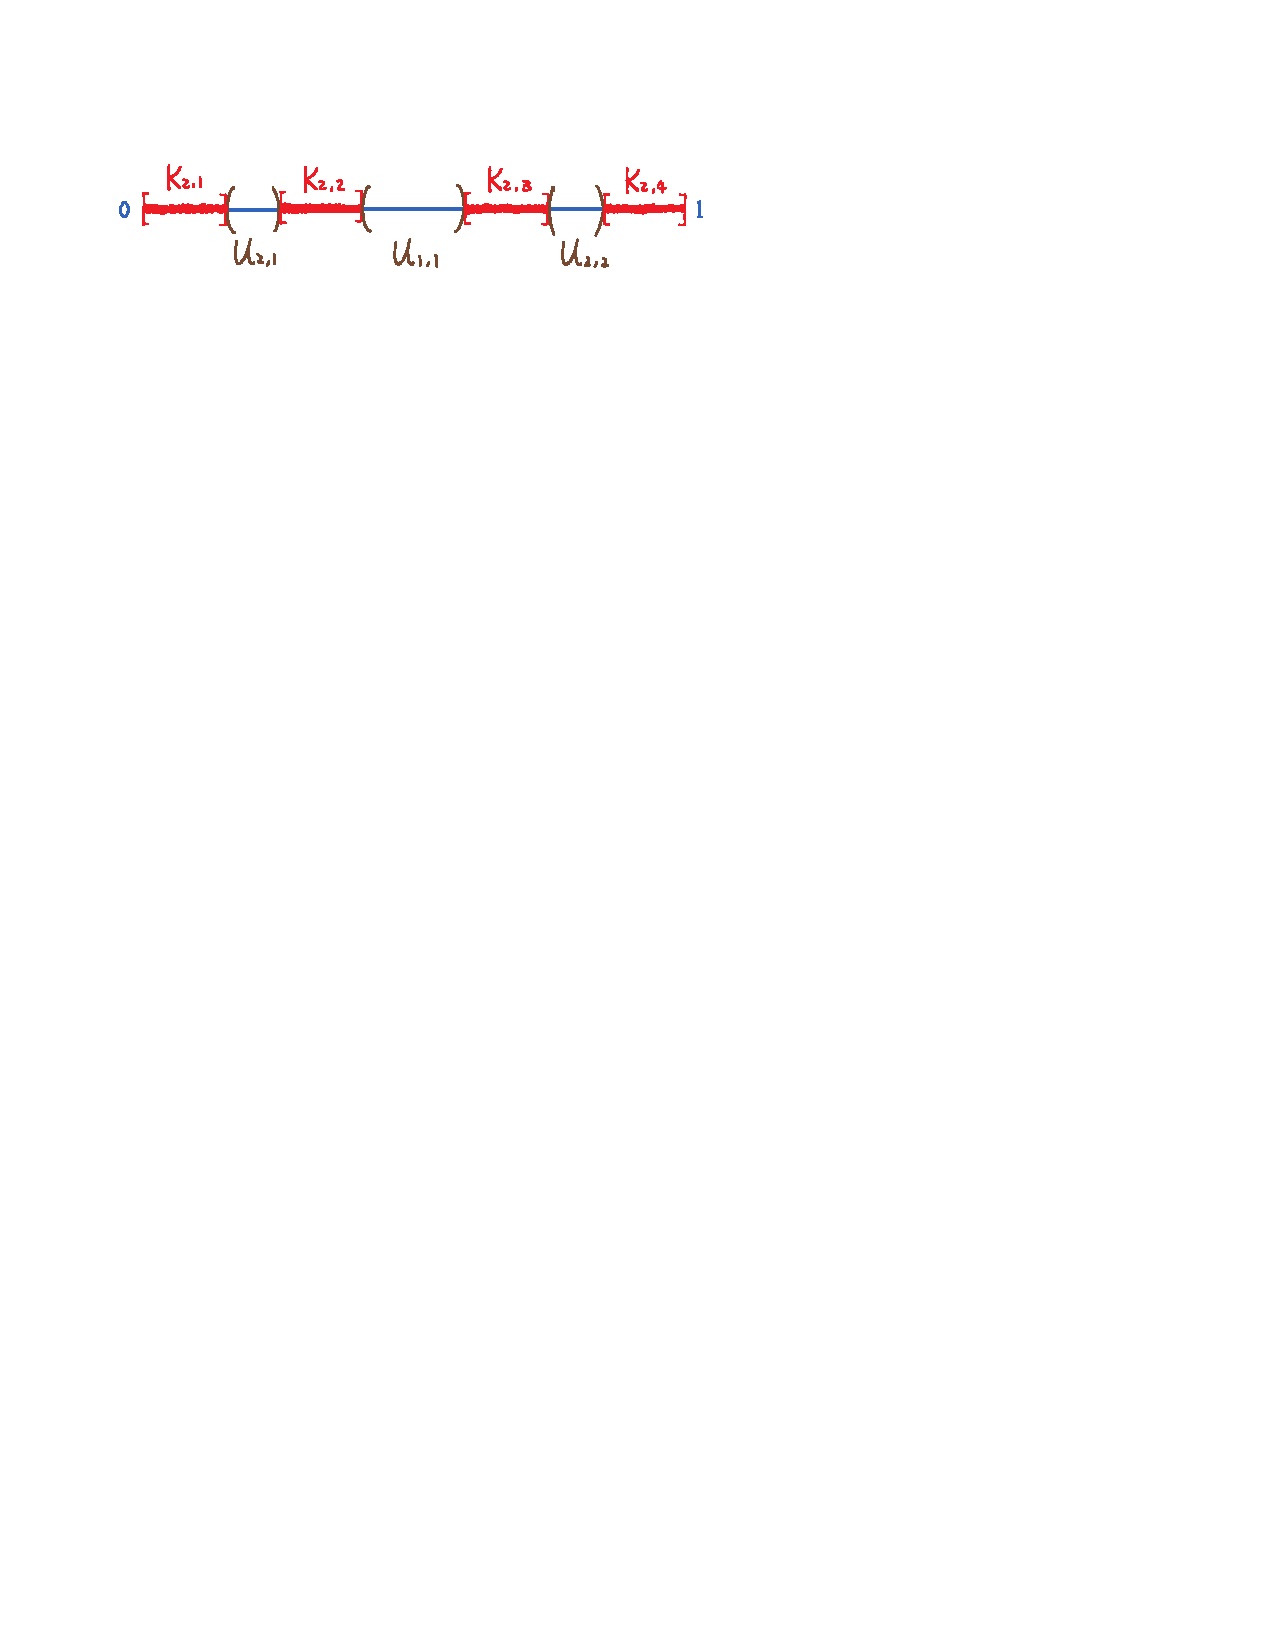
\includegraphics[scale=0.8]{cantor.pdf}
\end{center}
$l(K_{j,p})$ is independent of the choice of $p$, with $l(U_{j,p}) = \alpha_j\cdot l(K_{j-1},p)$. \\
Let $K_j =\bigcup_{i=1}^{2j} K_{j,i}$, and let $K =\bigcap_j K_j$. $K$ is called the generalized cantor set. 
\end{defn}

In the settings of the Definition. The generalized cantor set $K$ is compact, with empty interior, $U = [0,1]\setminus K$, which is the union of all $U_{j,p}$ defined in definition, $U\coloneqq \bigcup_{i,j} U_{i,j}$ is a dense open set. Pick $1 > n_1>n_2>\cdots>0$, one can pick $\alpha_j$ such that $m_{elem}(K_j) = n_j$, with the following holds:
\begin{align*}
m_{elem}(I\setminus K_j) = m_{elem}\left(\bigcup_{s\leq j,\ 1\leq p\leq 2j-1} U_{s,p}\right) = 1-{n_j}
\end{align*}
With results from Math 395 IBL6 Q3, we can write the following:
\begin{align*}
m_{*,J}(U) = \lim_{j \to \infty}{1-n_j} = 1-\lim_{j \to \infty} n_j \in (0,1]
\end{align*}
With results from Math 395 IBL6 Q1, we can write the following:
$$m^{*,J} (U) = m^{*,J} (\bar{U}) = 1$$
Here $U$ is Jordan measurable if and only if $\lim_{j \to \infty} n_j = 0$. Note that, between any two components of $U$, there infinitely many other components of $U$. Also note that, $Bd(U_{s,p}) \subseteq K$, and we see that the set $\bigcup_{s,p} (Bd(U_{s,p}))$ is countable, but $K$ is not countable because there is a surjection from $K$ to $[0,1]\times [0,1]$, so we know that most points of $K$ are not boundary points of some $U_{s,p}$, but we still have $K=Bd(K) = Bd(U)$. Moreover, with the settings given above, we can write the following:
\begin{align*}
n_j = (1-\alpha_j) = n_{j-1}
\end{align*}
with induction argument, we conclude:
$$n_j= (1-\alpha_1)(1-\alpha_2)\cdots (1-\alpha_j)$$
Hence we have the following holds:
\begin{align*}
\lim_{j\to \infty} n_j = \lim_{N \to \infty} \prod_{j=1}^N (1-\alpha_j) \coloneqq \prod_{j=1}^\infty (1-\alpha_j)
\end{align*}
hence we conclude that we have: 
$$m^*(K) = m^{*,J}(K) = 1-m_{*,J}(U) = 1-(1-\lim_{j\to \infty} n_j) = \lim_{j\to \infty} n_j$$
$$m^*(K) > 0 \iff \sum_{j=1}^\infty \alpha_j < \infty$$
Here we see that if $\alpha_j$ is independent of $j$, then $m^*(K) = 0$, and in the case where we have $\alpha_j = 2^{-j}$, we also have $m^*(K) = 0$. In fact, each $K$ is compact, each $x \in K$ is the limit of a sequence in $K \setminus \{x\}$. All connected subsets of $K$ are singletons.
\begin{thm}
Every metric spaces $X$ with the following properties is homeomorphic to the general cantor set $K$:
\begin{enumerate}
\item $X$ is compact
\item Each $x \in X$ is the limit of some sequence in $K\setminus \{x\}$
\item All connected subsets of $K$ are singletons
\end{enumerate}
\end{thm}

Given a vector space $V$, let $S$ be a vector subspace of $V$, let $\vec{a}\in V$, then $S+\vec{a}$ is an affine subset of $V$, $S$ is the vector subspace associated to $S+\vec{a}$. Here we define the followings:
\begin{defn}
Given a vector space $V$, let $S$ be a vector subspace of $V$, let $\vec{a}\in V$, $V\mid S\coloneqq$ the collection of all $S+\vec{a}$ is called the quotient space. 
\end{defn}
\exercise Given a vector space $V$, let $S$ be a vector subspace of $V$, $V\mid S$ is a vector space. One can write the followings:
\begin{align*}
(S+\vec{a})+(S+\vec{b}) = S+(\vec{a}+\vec{b}) \qquad\qquad\qquad \lambda(S+\vec{a}) = S+\lambda\vec{a}
\end{align*}
with $\vec{a},\vec{b}\in V$, and $\lambda\in F$ where $F$ is the field of $V$.\\

\begin{defn}
$Q_s: V \to V\mid 6S \ \ \ \ \vec{a}\mapsto S+\vec{a}$
\end{defn} 
\exercise $Q_s$ is linear and surjective. $\ker(Q_s) = S$. $T_V \to U$ is linear with $T|_S 0$, which induces $\that{T}:V\mid S \to W$, $T = \that{T}\circ Q_S$.

\newpage
$k$-form on manifold $M$ is a map $\omega$ with $\omega(\vec{p}) \in Alt^k(\T_p M)$ for all $\vec{p}\in M$. \\

In the following discussion, we assume that all maps are $C^\infty$ type.\\

When $k>\dim (M)$, then $Alt^k(\T_pM) = 0$.\\ 

There exists operators $d_k:\{k-\text{forms on }M\} \to \{(k+1)-\text{forms on }M\}$ such that we have (1) $d_{k+1}\circ d_{k} = 0$, and (2) Stokes' Theorem holds. \\

Here (1) implies that the image of $k_{k+1}$ is contained in the kernel of $d_k$. Here the dimension of the quotient $\frac{\ker(d_k)}{im(d_{k-1})}$ is called the $k$-th Betti Number $b_k(M)$. Notice that $d_0 f = 0$ if and only if $f$ is a constant function on each component, and here $b_0(M) = $ number of components. \\

Focus now on compact connected $1$-manifold. If we have $d_1 = 0$, then $\ker(d_1)$ is all $1$-manifold on $M$. $M$ is diffeomorphic to $I = [0,1]$ or $S^1$. On $I$, every $1$-form is $dg$ for some $0$-form $g$, so we have $b_1(I) = 0$. On $S^1$, one might consider $\beta: \R \to S^1 \ \ \ x\mapsto (\cos(x),\sin(x))$, with $\omega$ being $1$-form on $S^1$, we have $\beta^*S$ being $1$-form on $\R$. Here we can write $\beta^*\omega = f(x)\, dx$ with $f(x+2\pi) = f(x)$. $\omega = dg$ on $S^1$ implies $f(x)dx = \beta^* \omega = \beta^* dg = d\beta^* g = d(g\circ \beta) = (g\circ \beta)'(x)$ on $\R$. Here we need antiderivative for $f$ of the form $g\circ \beta$, need $h(x+2\pi) = h(x)$
\exercise $h(x+2\pi) -h(x) = \int_{S^1} \omega$. \\
\exercise $\{1-\text{forms on } S^1\} \to \R \ \ \ \omega\mapsto\int_{S^1} \omega$ induces isomorphism from the quotient $\frac{\ker(d_1)}{im(d_0)} \to \R$. \\

For $k=2$, here we will focus on $M$ compact without boundary. There are the following kinds of such:\\
(1) Sphere with $g$ handles, $b_1 = 2g$, $b_2 = 1$.\\
(2) Projection plane with $g$ handles, $b_1 = 2g$, $b_2 = 0$.\\
(3) Klein bottle with $g$ handles, $b_1 = 2g+1$, $b_2 = 0$. \\
\begin{corL}
Connected compact $2$-manifolds without boundaris cassified to diffeomorphism by $b_1$ and $b_2$. 
\end{corL}

\exercise (Poincare)\\
$M$ being the Poincare. $M$ is a topological space. $M$ is a topological manifold. $M$ is a differentiable manifold diffeomorphic to $3$-manifold without boundaries in $\R^5$.\\ 
$$b_k(M) = \begin{cases} 1 & k=0,3 \\0 k=1,2\end{cases}$$
Note that this is the same for $b_k(S^3)$, but $M$ is not homeomorphic to $S^3$. 

\begin{thm}[Perelman's Theorem]
Given $M$ being a compact connected $3$-manifold without boundary, and given that every continuous map from $S^1$ to $M$ extends to continuous map $B^2$ (ball) to $M$. Then $M$ is diffeomorphic to $S^3$.  
\end{thm}

For $k=4$, there exists compact connected topological $4$-manifold without boundary that is not homeomorphic to any differentiable manifold. (Freedman 1982) There exists open subset $A$ of $\R^4$ with $A$ being homeomorphic to $\R^4$ but not diffeomorphic to $\R^4$.\\ 

\begin{defn}
An $\R$-action on a set $S$ is a map $G:S \times \R \to S$ that satisfies $G(x,0) = x$, and $G(G(x,t),s) = G(x,t+s)$. 
\end{defn}

\exercise For $S^1$, $$G(\vec{x},t) = \bmat{\cos(t) & -\sin(t) \\ \sin(t) & \cos(t)}\vec{x}$$ defines an $\R$-action on $S^1$. \\

\exercise For $S^2 \subseteq \R^3$. 
$$G(\vec{x},t) = \bmat{\cos(t)& - \sin(t) & 0
\\sin(t)&\cos(t) &0
\\0&0&1}\vec{x}$$
defines an $\R$-action on $S^2$.\\

\exercise For $S^3 \in \R^4$,
$$G(\vec{x},t) = \bmat{\cos(t)& - \sin(t) & 0 &0
\\sin(t)&\cos(t) &0 & 0
\\0&0&\cos(t)&-\sin(t)
\\0&0&\sin(t) & \cos(t)}\vec{x}$$
defines an $\R$-action on $S^3$. 

\begin{defn}
An equilibirum point for the group action $G:S \times \R \to S$ is a point $x \in S$ such that $G(x,t) = x$ for all $t \in \R$. 
\end{defn}

\exercise $$G(\vec{x},t) = \bmat{\cos(t) & -\sin(t) \\ \sin(t) & \cos(t)}\vec{x}$$ 
has no equilibrium point.
$$G(\vec{x},t) = \bmat{\cos(t)& - \sin(t) & 0
\\sin(t)&\cos(t) &0
\\0&0&1}\vec{x}$$
has equilibrium points $(0,0,\pm 1)$.
$$G(\vec{x},t) = \bmat{\cos(t)& - \sin(t) & 0 &0
\\sin(t)&\cos(t) &0 & 0
\\0&0&\cos(t)&-\sin(t)
\\0&0&\sin(t) & \cos(t)}\vec{x}$$
has no equilibrium point.\\

Similarly to the exercises above, one can easily write down $\R$-actions on $S^n$ without equilibrium point if $n$ is odd. 

\begin{thm}[See You All in Math 396 Theorem]
When $n$ is even, any $C^\infty$ type $\R$-action on $S^n$ has at list one equilibrium point.
\end{thm}

Given $\R$-action on $M$, for $x \in M$, we can write the following:
$$\left.\frac{\partial }{\partial t}G(x,t) \right|_{t=0} \in \T_x(M) = x^\perp$$
A map taking $x \in M$ to $f(x) \in \T_x(M)$ is called a vector field. 

\begin{thm}
For $M$ compact manifold without boundary, the map $\{\R-\text{actions on } M\}\to \{\text{vector field on }M\}$ given above is a bijection. 
\end{thm}


\newpage
\section{Math 396}

Let $\omega$ be a $1$-form on an open subset $A$ of $\R^n$, here $\omega$ defines a function from $A$ to $(\R^n)^* = \hom(\R^n, \R)$. For $\vec{p}\in A$, we have $\omega(\vec{p}):\R^n \to \R$, and $\dim(\ker(\omega(\vec{p}))) = n-1$ or $n$. 
\begin{prop}
For $k$-manifold $M$ being a subset of an open subset $A$ of $\R^n$, the followings are equivalent:
\begin{enumerate}
\item $\T_{\vec{p}}(M) \subseteq \ker(\omega(\vec{p}))$ for all $\vec{p}\in M$
\item $\alpha^*\omega = 0$ for all coordinate patches $\alpha$ for $M$
\item $\int_C \omega =0$ for all $1$-manifold $C\subseteq M$. 
\end{enumerate} 
\end{prop}
\begin{proof}
The proof of this proposition is given in Math 396 HW1. 
\end{proof}

\begin{defn}
Let $\omega$ be a $1$-form on an open subset $A$ of $\R^n$, for $k$-manifold $M \subseteq A$, $M$ is said to be an integral manifold for $\omega$ provided that $\int \omega =0$ for all $1$-manifold $C\subseteq M$. 
\end{defn}

Integral manifolds for $\omega$ are also integral manifold for $g\omega$ where $g$ is a scalar function. Note that $\alpha^*(g\omega) = (\alpha^*g)(\alpha^*\omega)$. \\

\begin{lem}
Let $f \in C^1(A,\R)$ where $A$ is an open subset of $\R^n$, with $df \neq 0$ on $A$. \\Then, for $c \in \R$, the level set $f^{-1}(c)$ is $(n-1)$-manifold without boundary.
\end{lem}
\begin{proof}
The proof of this lemma is given in Theorem I.6 on Math 396 Supplement Materials. 
\end{proof}

\begin{corL}
Let $f \in C^1(A,\R)$ where $A$ is an open subset of $\R^n$, with $df \neq 0$ on $A$.\\
Each level set of $f$ is an integral manifold for $df$.
\end{corL}
\begin{proof}
$\alpha^*(df) = d(\alpha^* f) = d(f\circ \alpha) = d(c) = 0$ for some $c \in \R$. 
\end{proof}


Let $\omega = U(x,y)\, dx + V(x,y) \, dy$ be defined on an open subset $A$ of $\R^2$, with functions $U:\R^2 \to \R$, $V:\R^2 \to \R$. Let $V$ be non-vanishing on $A$. Let $f \in C^1((a,b),\R)$ with $M\coloneqq Graph(f) \subseteq A$. Let $\alpha:(a,b) \to M \ \ \ x\mapsto (x,f(x))$. \\

$M$ is an integral manifold for $\omega$ if and only if $\alpha^* \omega = 0$, where $\alpha^*\omega = (U(x,f(x))+V(x,f(x))f'(x))\, dx =0$ if and only if $f'(x) =- \frac{U(x,f(x))}{V(x,f(x))}$. \\

Suppose $U,V \in C^1(\R^2,\R)$, then $-\frac{U(x,y)}{V(x,y)} \in C^1$, consider the point $(0,y_0) \in A$, we claim that there exists $\psi \in C^1(\R^2,\R)$ with bounded function $D\psi :\R^2 \to \R^2_{row}$ such that $\psi (x,y) = -\frac{U(x,y)}{V(x,y)}$ for $(x,y)$ in the neighborhood of $(0,y_0)$. Pick $\eta \in C^\infty (\R^2, \R)$ with $\eta(x,y) = 1$ in neighborhood of $(0,y_0)$ such that $supp(\eta)$ is a compact support of $A$. Define the following:
$$\psi(x,y) = \begin{cases}-\frac{U(x,y)}{V(x,y)}\eta(x,y) & (x,y) \in A \\ 0 &(x,y) \notin A \end{cases}$$
Here $D\psi$ is bounded because it has compact support, and it satisfies the conditions in the claim. By Math 395 HW4 Q6, $\psi$ is Lipchitz on $\R^2$, hence is partially Lipschitz on $\R^2$. By Math 395 HW10 Q5, $\exists\ \epsilon>0$ such that $f'(x) = \psi(x,f(x))$ has a unique solution on $(-\epsilon,\epsilon)$. One can shrink $\epsilon$ if necessary to $\bar{\epsilon}>0$ such that $f'(x) = -\frac{U(x,f(x))}{V(x,f(x))}$ has unique solution on $(-\bar{\epsilon},\bar{\epsilon})$, so there exists a unique local integral curve for $\omega$ passing through $(0,y_0)$. We claim that we get the same result for each $(x_0,y_0) \in A$, one can show by using a translation in the $x$-direction. \\

For continuous functions $U$ and $V$, one can show that the solutions guaranteed to exist, but the uniqueness can fail. One example is given by Math 395 HW11 Q5.\\

Conversely given differential equation: 
\begin{align*}
f'(x) = \psi(x,f(x)) \tag(D)
\end{align*}
then the graphs of solutions of (D) are integral curves for $\omega \coloneqq -\psi(x,y)dx+dy$ and for $\that{\omega} = B(x,y) \omega = -B(x,y)\psi(x,y)\, dx + B(x,y)\, dy$. If $\that{\omega}$ is exact, that is, if $\that{\omega} = dg$ for some function $g$, then $B$ is an integrating factor for $\omega$. Since level curves $g^{-1}(c)$ are integral manifolds for $dg = \that{\omega}$, assuming $B \neq 0$, then $g^{-1}(c)$ are also integral manifolds for $\omega = \psi(x,y)\, dx + dy$, and hence $g^{-1}(c)$ are graphs of solutions of (D).\\

Conversely, suppose $f$ solves the differential equation (D), then we can write the following:
\begin{align*}
\frac{d}{dx} g\bmat{x \\ f(x)} &= dg\left(\bmat{x\\ f(x)}\right) \cdot \bmat{1 \\ f'(x)} \\
&= \bmat{-B\left(\bmat{x \\ f(x)} \right)\psi\left(\bmat{x \\ f(x)} \right) & B\left(\bmat{x \\ f(x)} \right)} \cdot \bmat{1 \\ f'(x)} \\
&= -B\left(\bmat{x\\ f(x)}\right) \psi\left( \bmat{x\\f(x)}\right) + B\left( \bmat{x\\ f(x)}\right) f'(x) = 0
\end{align*}
Here we see that $g\left(\bmat{x \\f(x)} \right)$ is locally constant.

The good news are, such $B$ always exists, looking for $B$ is often useful when solving differential equation (D), but the bad news is find $B$ is not always easier than trying to solve (D). 



\end{document}
